%%%%%%%%%%%%%%%%%%%%%%%%%%%%%%%%%%%%%%%%%%%%%%%%%%%%%%%%%%%%%%%%%%%%%%%%%%%%
%%%%%                          ANNEXE 1                               %%%%%%
%%%%%%%%%%%%%%%%%%%%%%%%%%%%%%%%%%%%%%%%%%%%%%%%%%%%%%%%%%%%%%%%%%%%%%%%%%%%

\appendix
\renewcommand\chaptername{Annexe~}
% \phantomsection

\lhead[\fancyplain{}{\leftmark}]%Pour les pages paires \bfseries
      {\fancyplain{}{}} %Pour les pages impaires
\chead[\fancyplain{}{}]%
      {\fancyplain{}{}}
\rhead[\fancyplain{}{}]%Pour les pages paires 
      {\fancyplain{}{\rightmark}}%Pour les pages impaires \bfseries
\lfoot[\fancyplain{}{}]%
      {\fancyplain{}{}}
\cfoot[\fancyplain{}{\thepage}]%\bfseries
      {\fancyplain{}{\thepage}} %\bfseries
\rfoot[\fancyplain{}{}]%
     {\fancyplain{}{\scriptsize}}


%%%%%%%%%%%%%%%%%%%%%%%%%%%%%%%%%%%%%%%%%%%%%%%%%%%%%%%%%%%%%%%%%%%%%%%%%%
%%%%%                      Start part here                          %%%%%%
%%%%%%%%%%%%%%%%%%%%%%%%%%%%%%%%%%%%%%%%%%%%%%%%%%%%%%%%%%%%%%%%%%%%%%%%%%

\chapter{Maîtrise du procédé d'injection-moulage des thermoplastiques}
\label{Ann:process_control}

%==============================================================================	Résumé du chapitre

\begin{center}
\rule{0.7\linewidth}{.5pt}
\begin{minipage}{0.7\linewidth}
\smallskip

\textit{
Cette annexe propose une étude bibliographique de la maîtrise du procédé d'injection-moulage des thermoplastiques, de 1975 à 2015.
}

%\smallskip
\end{minipage}
\smallskip
\rule{0.7\linewidth}{.5pt}
\end{center}

%\adjustmtc
% \minitoc
% \newpage
\bigskip

Cette annexe est complémentaire de la Section \ref{subsec:process_control} "Maîtrise du procédé d'injection-moulage des thermoplastiques" du Chapitre \ref{ch:objectives}.
L'objectif de la maîtrise d'un procédé est de maîtriser la qualité du produit : c'est à dire de limiter la dispersion des caractéristiques des pièces.
Il s'agit en priorité d'effectuer des mesures pertinentes sur l'état du procédé, puis de les analyser afin de détecter les dérives.
Une dernière étape est l'ajustement automatique des paramètres du procédé.

\begin{figure}[htbp]
	\centering
	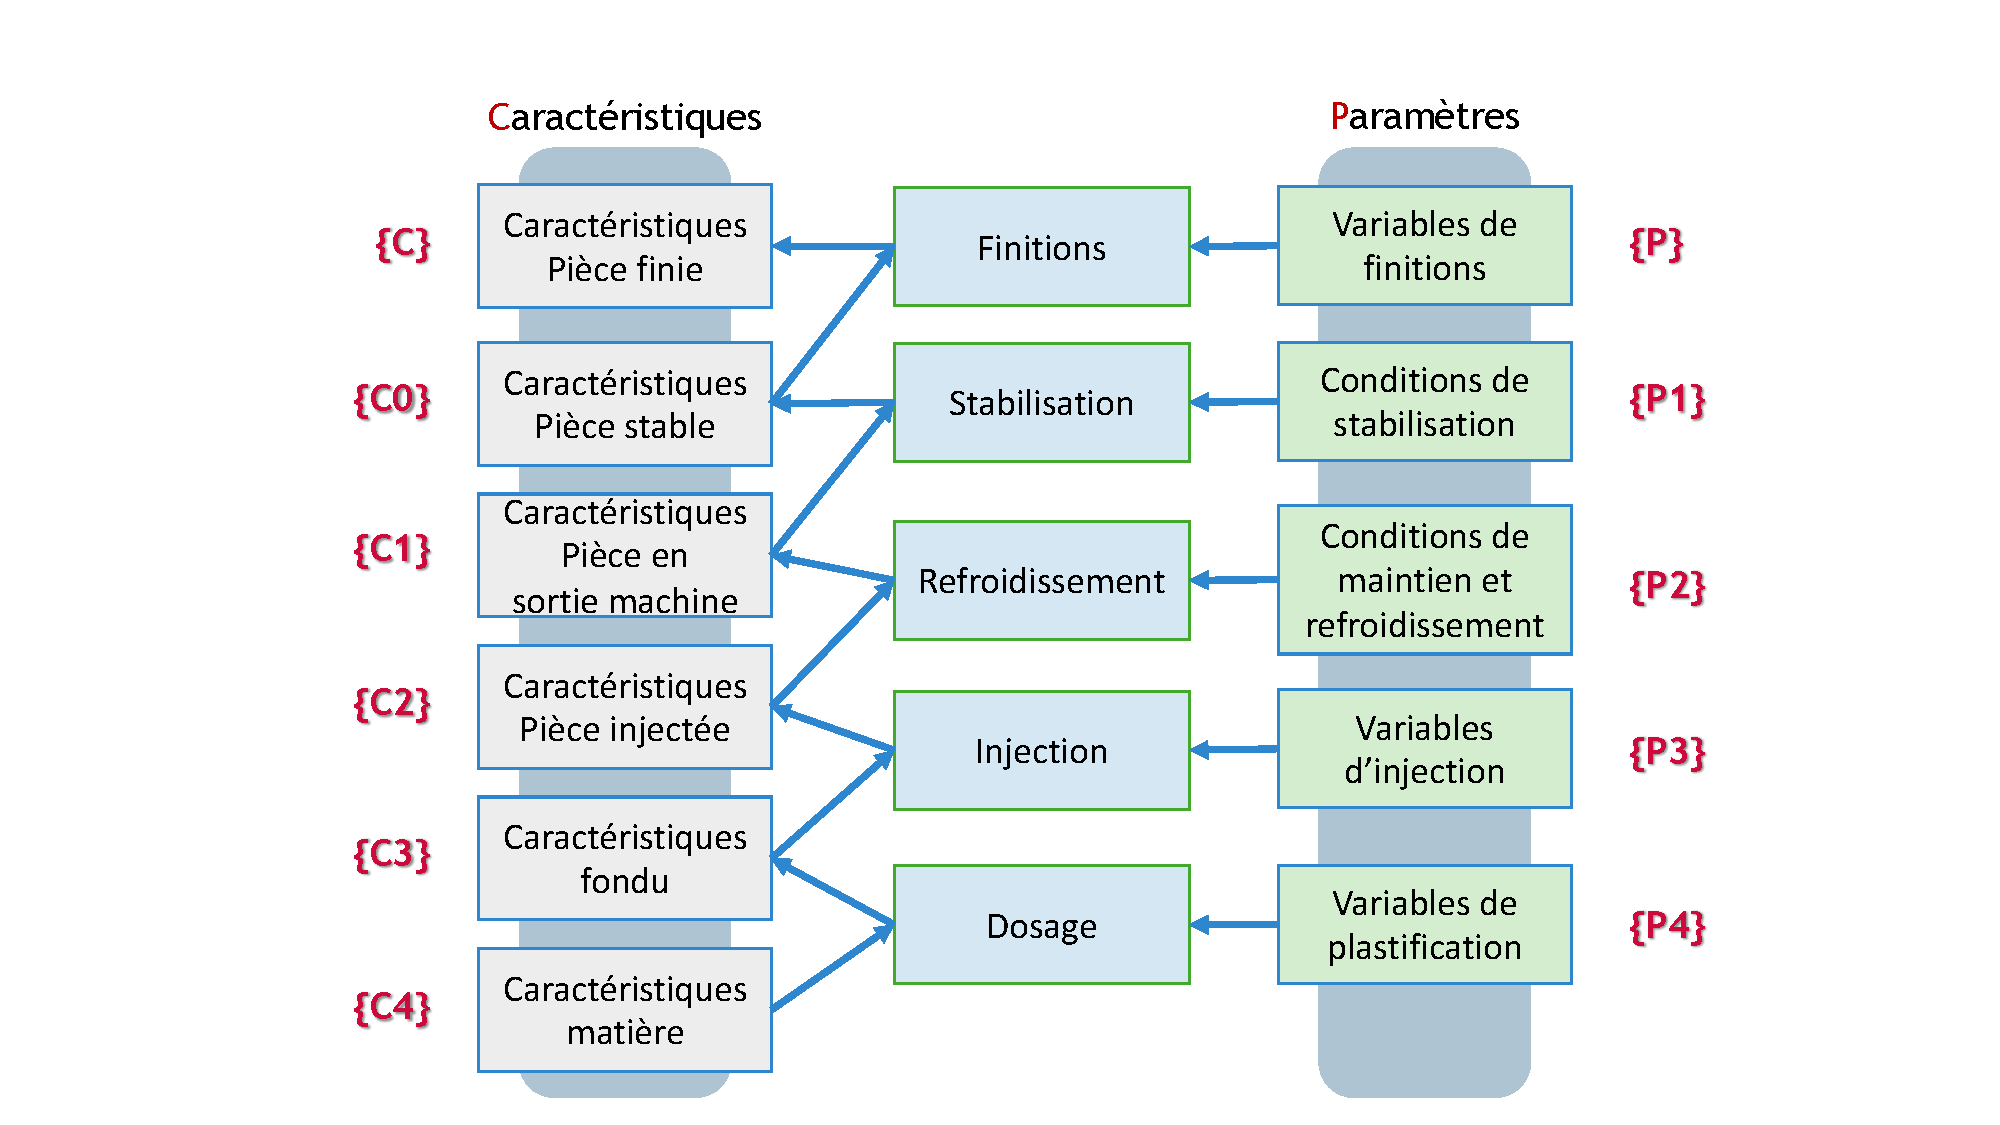
\includegraphics[width=0.80\textwidth,height=\textheight,keepaspectratio]{../Chap1/Figures/Sapristi_ZigZag.pdf}
	\caption{Représentation \textit{Zig Zag} du procédé d'injection-moulage des thermoplastiques.}
	\label{fig:annexe_zigzag}
\end{figure}

%\begin{figure}[hbtp]
%	\centering
%	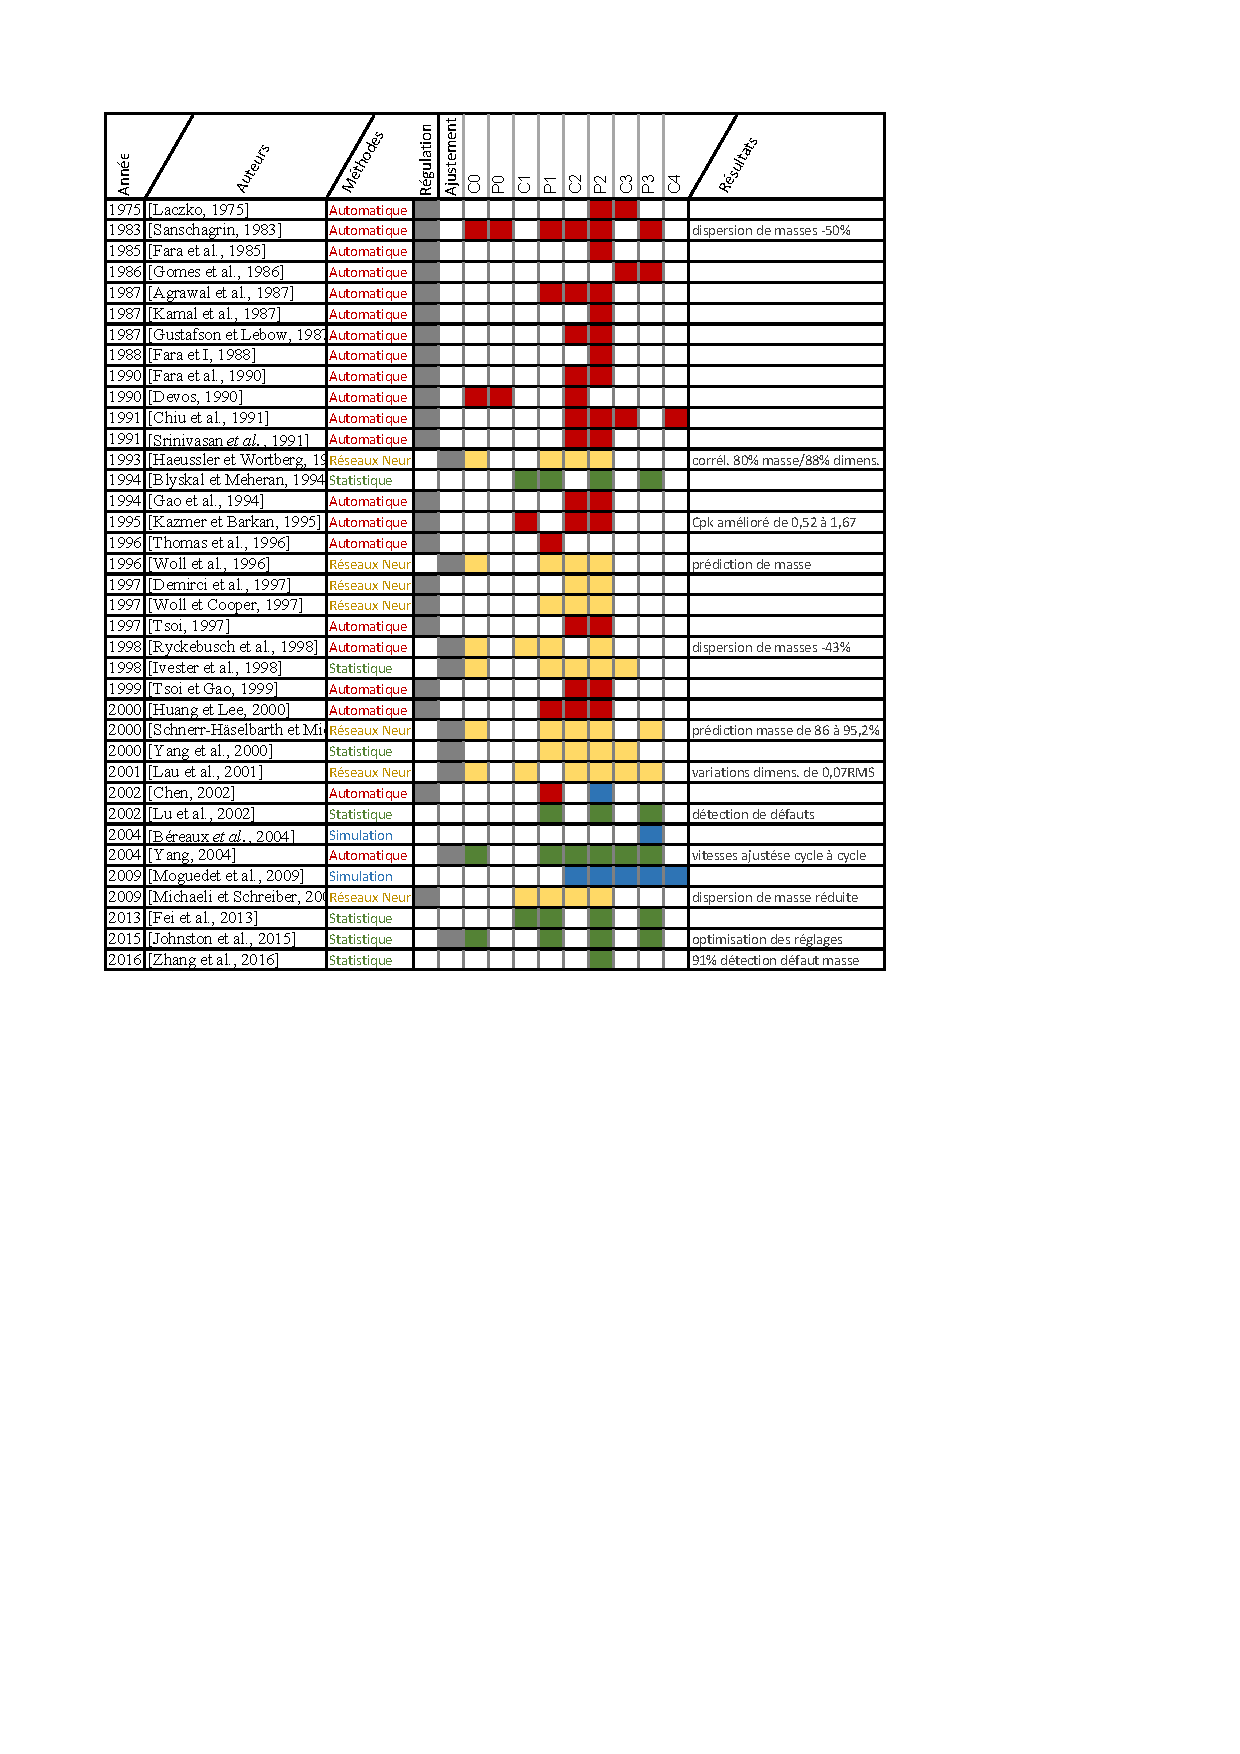
\includegraphics[width=\textwidth,height=\textheight,keepaspectratio]{../Chap1/Figures/TableauComparaisonEssais.pdf}
%	\caption{Cartographie bibliographique de la maîtrise du procédé d'injection-moulage.}
%	\label{tab:state_art_compare}
%\end{figure}

% from https://tex.stackexchange.com/a/416169
% \newcommand{\STAB}[1]{\begin{tabular}{@{}r@{}}#1\end{tabular}}
\newcommand{\bcline}[1]{\arrayrulecolor{black}\cline{#1}\arrayrulecolor{black}}
\begin{table}[hbtp]
	\centering
	\resizebox{\textwidth}{!}{%
		\begin{tabular}{!{\color{black}\vrule}l l l l!{\color{black}\vrule}l!{\color{gray}\vrule}l!{\color{gray}\vrule}l!{\color{gray}\vrule}l!{\color{gray}\vrule}l!{\color{gray}\vrule}l!{\color{gray}\vrule}l!{\color{gray}\vrule}l!{\color{gray}\vrule}l!{\color{black}\vrule}}
			\bcline{5-13} \multicolumn{1}{l}{} &                                &                                           &                                & \rotatebox[origin=r]{90}{Caractéristiques de la pièce stable} & \rotatebox[origin=r]{90}{Paramètres de stabilisation} & \rotatebox[origin=r]{90}{Caractéristiques de la pièce chaude} & \rotatebox[origin=r]{90}{Param. de maintien-refroidissement} & \rotatebox[origin=r]{90}{Caractéristiques de la pièce injectée} & \rotatebox[origin=r]{90}{Paramètres d'injection} & \rotatebox[origin=r]{90}{Caractéristiques de la matière fondue} & \rotatebox[origin=r]{90}{Paramètres de plastification} & \rotatebox[origin=r]{90}{Caractéristiques de la matière initiale} \\ \bcline{1-4}
			\multicolumn{1}{!{\color{black}\vrule}l!{\color{black}\vrule}}{Année} & \multicolumn{1}{l!{\color{black}\vrule}}{Auteurs [Publication]}   & \multicolumn{1}{l!{\color{black}\vrule}}{Méthode utilisée}     & \multicolumn{1}{l!{\color{black}\vrule}}{Objectif}       & $\boldsymbol{C}_0$                              & $\boldsymbol{P}_1$                              & $\boldsymbol{C}_1$       & $\boldsymbol{P}_2$       & $\boldsymbol{C}_2$       & $\boldsymbol{P}_3$                              & $\boldsymbol{C}_3$       & $\boldsymbol{P}_4$       & $\boldsymbol{C}_4$       \\ \bcline{1-13}
			1975                        & \citeauthor{laczko_controller_1975} \cite{laczko_controller_1975}                         & {\color[HTML]{CB0000} Automatique}        & {\color[HTML]{CE6301} Régulation}   &                                                 &                                                 &                          &                          &                          & \cellcolor[HTML]{CB0000}                        & \cellcolor[HTML]{CB0000} &                          &                          \\
			1983                        & \citeauthor{sanschagrin_process_1983} \cite{sanschagrin_process_1983}                    & {\color[HTML]{CB0000} Automatique}        & {\color[HTML]{CE6301} Régulation}   & \cellcolor[HTML]{CB0000}                        & \cellcolor[HTML]{CB0000}                        &                          & \cellcolor[HTML]{CB0000} & \cellcolor[HTML]{CB0000} & \cellcolor[HTML]{CB0000}                        &                          & \cellcolor[HTML]{CB0000} &                          \\
			1985                        & \citeauthor{fara_evaluation_1985} \cite{fara_evaluation_1985} & {\color[HTML]{CB0000} Automatique}        & {\color[HTML]{CE6301} Régulation}   &                                                 &                                                 &                          &                          &                          & \cellcolor[HTML]{CB0000}                        &                          &                          &                          \\
			1986                        & \citeauthor{gomes_injection_1986} \cite{gomes_injection_1986} & {\color[HTML]{CB0000} Automatique}        & {\color[HTML]{CE6301} Régulation}   &                                                 &                                                 &                          &                          &                          &                                                 & \cellcolor[HTML]{CB0000} & \cellcolor[HTML]{CB0000} &                          \\
			1987                        & \citeauthor{agrawal_injection-molding_1987} \cite{agrawal_injection-molding_1987} & {\color[HTML]{CB0000} Automatique}        & {\color[HTML]{CE6301} Régulation}   &                                                 &                                                 &                          & \cellcolor[HTML]{CB0000} & \cellcolor[HTML]{CB0000} & \cellcolor[HTML]{CB0000}                        &                          &                          &                          \\
			1987                        & \citeauthor{kamal_dynamics_1987} \cite{kamal_dynamics_1987} & {\color[HTML]{CB0000} Automatique}        & {\color[HTML]{CE6301} Régulation}   &                                                 &                                                 &                          &                          &                          & \cellcolor[HTML]{CB0000}                        &                          &                          &                          \\
			1987                        & \citeauthor{gustafson_model_1987} \cite{gustafson_model_1987} & {\color[HTML]{CB0000} Automatique}        & {\color[HTML]{CE6301} Régulation}   &                                                 &                                                 &                          &                          & \cellcolor[HTML]{CB0000} & \cellcolor[HTML]{CB0000}                        &                          &                          &                          \\
			1988                        & \citeauthor{fara_control_1988} \cite{fara_control_1988}                        & {\color[HTML]{CB0000} Automatique}        & {\color[HTML]{CE6301} Régulation}   &                                                 &                                                 &                          &                          &                          & \cellcolor[HTML]{CB0000}                        &                          &                          &                          \\
			1990                        & \citeauthor{fara_comprehensive_1990} \cite{fara_comprehensive_1990}                & {\color[HTML]{CB0000} Automatique}        & {\color[HTML]{CE6301} Régulation}   &                                                 &                                                 &                          &                          & \cellcolor[HTML]{CB0000} & \cellcolor[HTML]{CB0000}                        &                          &                          &                          \\
			1990                        & \citeauthor{devos_contribution_1990} \cite{devos_contribution_1990} & {\color[HTML]{CB0000} Automatique}        & {\color[HTML]{CE6301} Régulation}   & \cellcolor[HTML]{CB0000}{\color[HTML]{000000} } & \cellcolor[HTML]{CB0000}{\color[HTML]{000000} } &                          &                          & \cellcolor[HTML]{CB0000} &                                                 &                          &                          &                          \\
			1991                        & \citeauthor{chiu_dynamic_1991} \cite{chiu_dynamic_1991} & {\color[HTML]{CB0000} Automatique}        & {\color[HTML]{CE6301} Régulation}   &                                                 &                                                 &                          &                          & \cellcolor[HTML]{CB0000} & \cellcolor[HTML]{CB0000}                        & \cellcolor[HTML]{CB0000} &                          & \cellcolor[HTML]{CB0000} \\
			1991                        & Srinivasan et al.              & {\color[HTML]{CB0000} Automatique}        & {\color[HTML]{CE6301} Régulation}   &                                                 &                                                 &                          &                          & \cellcolor[HTML]{CB0000} & \cellcolor[HTML]{CB0000}                        &                          &                          &                          \\
			1993                        & \citeauthor{haeussler_quality_1993} \cite{haeussler_quality_1993} & {\color[HTML]{00009B} Réseau de Neurones} & {\color[HTML]{6200C9} Surveillance} & \cellcolor[HTML]{00009B}                        &                                                 &                          & \cellcolor[HTML]{00009B} & \cellcolor[HTML]{00009B} & \cellcolor[HTML]{00009B}                        &                          &                          &                          \\
			1994                        & \citeauthor{blyskal_applying_1994} \cite{blyskal_applying_1994} & {\color[HTML]{009901} Plan d'expériences} & {\color[HTML]{34696D} Pilotage}     &                                                 &                                                 & \cellcolor[HTML]{009901} & \cellcolor[HTML]{009901} &                          & \cellcolor[HTML]{009901}{\color[HTML]{000000} } &                          & \cellcolor[HTML]{009901} &                          \\
			1994                        & Gao et al.                     & {\color[HTML]{CB0000} Automatique}        & {\color[HTML]{CE6301} Régulation}   &                                                 &                                                 &                          &                          & \cellcolor[HTML]{CB0000} & \cellcolor[HTML]{CB0000}                        &                          &                          &                          \\
			1995                        & \citeauthor{kazmer_dynamic_1995} \cite{kazmer_dynamic_1995} & {\color[HTML]{CB0000} Automatique}        & {\color[HTML]{CE6301} Régulation}   &                                                 &                                                 & \cellcolor[HTML]{CB0000} &                          & \cellcolor[HTML]{CB0000} & \cellcolor[HTML]{CB0000}                        &                          &                          &                          \\
			1996                        & Thomas et al.                  & {\color[HTML]{CB0000} Automatique}        & {\color[HTML]{CE6301} Régulation}   &                                                 &                                                 &                          & \cellcolor[HTML]{CB0000} &                          &                                                 &                          &                          &                          \\
			1996                        & \citeauthor{woll_online_1996} \cite{woll_online_1996} & {\color[HTML]{00009B} Réseau de Neurones} & {\color[HTML]{6200C9} Surveillance} & \cellcolor[HTML]{00009B}                        &                                                 &                          & \cellcolor[HTML]{00009B} & \cellcolor[HTML]{00009B} & \cellcolor[HTML]{00009B}                        &                          &                          &                          \\
			1997                        & \citeauthor{demirci_numerical_1997} \cite{demirci_numerical_1997} & {\color[HTML]{00009B} Réseau de Neurones} & {\color[HTML]{CE6301} Régulation}   &                                                 &                                                 &                          &                          & \cellcolor[HTML]{00009B} & \cellcolor[HTML]{00009B}                        &                          &                          &                          \\
			1997                        & \citeauthor{woll_pattern-based_1997} \cite{woll_pattern-based_1997} & {\color[HTML]{00009B} Réseau de Neurones} & {\color[HTML]{CE6301} Régulation}   &                                                 &                                                 &                          & \cellcolor[HTML]{00009B} & \cellcolor[HTML]{00009B} & \cellcolor[HTML]{00009B}                        &                          &                          &                          \\
			1997                        & \cite{tsoi_fuzzy_1997} \citeauthor{tsoi_fuzzy_1997} & {\color[HTML]{CB0000} Automatique}        & {\color[HTML]{CE6301} Régulation}   &                                                 &                                                 &                          &                          & \cellcolor[HTML]{CB0000} & \cellcolor[HTML]{CB0000}                        &                          &                          &                          \\
			1998                        & Ryckebusch et al.              & {\color[HTML]{CB0000} Automatique}        & {\color[HTML]{CE6301} Régulation}   & \cellcolor[HTML]{CB0000}                        &                                                 & \cellcolor[HTML]{CB0000} & \cellcolor[HTML]{CB0000} &                          & \cellcolor[HTML]{CB0000}                        &                          &                          &                          \\
			1998                        & \citeauthor{ivester_automatic_1998} \cite{ivester_automatic_1998} & {\color[HTML]{009901} Plan d'expériences} & {\color[HTML]{6200C9} Surveillance} & \cellcolor[HTML]{009901}                        &                                                 &                          & \cellcolor[HTML]{009901} & \cellcolor[HTML]{009901} & \cellcolor[HTML]{009901}                        & \cellcolor[HTML]{009901} &                          &                          \\
			1999                        & \citeauthor{tsoi_real-time_1997} \cite{tsoi_real-time_1997} & {\color[HTML]{CB0000} Automatique}        & {\color[HTML]{CE6301} Régulation}   &                                                 &                                                 &                          &                          & \cellcolor[HTML]{CB0000} & \cellcolor[HTML]{CB0000}                        &                          &                          &                          \\
			2000                        & \citeauthor{huang_fuzzy_2000} \cite{huang_fuzzy_2000}                   & {\color[HTML]{CB0000} Automatique}        & {\color[HTML]{CE6301} Régulation}   &                                                 &                                                 &                          & \cellcolor[HTML]{CB0000} & \cellcolor[HTML]{CB0000} & \cellcolor[HTML]{CB0000}                        &                          &                          &                          \\
			2000                        & \citeauthor{schnerr-haselbarth_automation_2000} \cite{schnerr-haselbarth_automation_2000} & {\color[HTML]{00009B} Réseau de Neurones} & {\color[HTML]{6200C9} Surveillance} & \cellcolor[HTML]{00009B}                        &                                                 &                          & \cellcolor[HTML]{00009B} & \cellcolor[HTML]{00009B} & \cellcolor[HTML]{00009B}                        &                          & \cellcolor[HTML]{00009B} &                          \\
			2000                        & \citeauthor{yang_knowledgebased_2000} \cite{yang_knowledgebased_2000} & {\color[HTML]{009901} Plan d'expériences} & {\color[HTML]{6200C9} Surveillance} &                                                 &                                                 &                          & \cellcolor[HTML]{009901} & \cellcolor[HTML]{009901} & \cellcolor[HTML]{009901}                        & \cellcolor[HTML]{009901} &                          &                          \\
			2001                        & \citeauthor{lau_neural_2001} \cite{lau_neural_2001} & {\color[HTML]{00009B} Réseau de Neurones} & {\color[HTML]{6200C9} Surveillance} & \cellcolor[HTML]{00009B}                        &                                                 & \cellcolor[HTML]{00009B} &                          & \cellcolor[HTML]{00009B} & \cellcolor[HTML]{00009B}                        & \cellcolor[HTML]{00009B} & \cellcolor[HTML]{00009B} &                          \\
			2002                        & \citeauthor{chen_study_2002} \cite{chen_study_2002} & {\color[HTML]{CB0000} Automatique}        & {\color[HTML]{CE6301} Régulation}   &                                                 &                                                 &                          & \cellcolor[HTML]{CB0000} &                          & \cellcolor[HTML]{CB0000}                        &                          &                          &                          \\
			2003                        & \citeauthor{pillet_maitrise_2003} \cite{pillet_maitrise_2003} & {\color[HTML]{009901} MSP}                & {\color[HTML]{6200C9} Surveillance} &                                                 &                                                 & \cellcolor[HTML]{009901} & \cellcolor[HTML]{009901} & \cellcolor[HTML]{009901} & \cellcolor[HTML]{009901}                        &                          &                          &                          \\
			2004                        & \citeauthor{lu_stagebased_2004} \cite{lu_stagebased_2004} & {\color[HTML]{009901} Plan d'expériences} & {\color[HTML]{6200C9} Surveillance} &                                                 &                                                 &                          & \cellcolor[HTML]{009901} &                          & \cellcolor[HTML]{009901}                        &                          & \cellcolor[HTML]{009901} &                          \\
			2004                        & \citeauthor{yang_injection_2004} \cite{yang_injection_2004} & {\color[HTML]{CB0000} Automatique}        & {\color[HTML]{6200C9} Surveillance} & \cellcolor[HTML]{CB0000}                        &                                                 &                          & \cellcolor[HTML]{CB0000} & \cellcolor[HTML]{CB0000} & \cellcolor[HTML]{CB0000}                        & \cellcolor[HTML]{CB0000} & \cellcolor[HTML]{CB0000} &                          \\
			2006                        & \citeauthor{fournier_conduite_2006} \cite{fournier_conduite_2006} & {\color[HTML]{CB0000} Automatique}        & {\color[HTML]{34696D} Pilotage}     & \cellcolor[HTML]{CB0000}                        &                                                 & \cellcolor[HTML]{CB0000} & \cellcolor[HTML]{CB0000} &                          & \cellcolor[HTML]{CB0000}                        &                          &                          &                          \\
			2009                        & \citeauthor{michaeli_online_2009} \cite{michaeli_online_2009} & {\color[HTML]{00009B} Réseau de Neurones} & {\color[HTML]{CE6301} Régulation}   &                                                 &                                                 & \cellcolor[HTML]{00009B} & \cellcolor[HTML]{00009B} & \cellcolor[HTML]{00009B} & \cellcolor[HTML]{00009B}                        &                          &                          &                          \\
			2013                        & \citeauthor{fei_practical_2013} \cite{fei_practical_2013} & {\color[HTML]{009901} Plan d'expériences} & {\color[HTML]{6200C9} Surveillance} &                                                 &                                                 & \cellcolor[HTML]{009901} & \cellcolor[HTML]{009901} &                          & \cellcolor[HTML]{009901}                        &                          & \cellcolor[HTML]{009901} &                          \\
			2014                        & Zhao et al.                    & {\color[HTML]{009901} MSP}                & {\color[HTML]{6200C9} Surveillance} &                                                 &                                                 &                          &                          &                          & \cellcolor[HTML]{009901}                        & \cellcolor[HTML]{009901} &                          &                          \\
			2015                        & \citeauthor{johnston_-line_2015} \cite{johnston_-line_2015} & {\color[HTML]{34696D} Pilotage} & {\color[HTML]{6200C9} Surveillance} & \cellcolor[HTML]{009901}                        &                                                 &                          & \cellcolor[HTML]{009901} &                          & \cellcolor[HTML]{009901}                        &                          & \cellcolor[HTML]{009901} &                          \\
			2016                        & \citeauthor{zhang_statistical_2016} \cite{zhang_statistical_2016} & {\color[HTML]{009901} MSP}                & {\color[HTML]{6200C9} Surveillance} &                                                 &                                                 &                          &                          &                          & \cellcolor[HTML]{009901}                        &                          &                          &                          \\
			2017                        & Zhou et al.                    & {\color[HTML]{CB0000} MSP \& Auto.}       & {\color[HTML]{34696D} Pilotage}     &                                                 &                                                 & \cellcolor[HTML]{CB0000} &                          &                          & \cellcolor[HTML]{CB0000}                        & \cellcolor[HTML]{CB0000} &                          &                          \\
			\bcline{1-13}
		\end{tabular}%
	}
	\caption{Récapitulatif de l'étude bibliographique.}
	\label{tab:state_art_compare}
\end{table}

Cette annexe propose une étude bibliographique des techniques de maîtrise du procédé d'injection-moulage.
Le Tableau \ref{tab:state_art_compare} récapitule cette revue de la littérature.

La maîtrise d'un procédé de production peut être discrétisée en différentes étapes :
\begin{enumerate}
	\item réglage initial d'un point de fonctionnement (paramètres $\boldsymbol{P}_{2-4}$) : connaissance humaine et système expert,
	\item régulation du point de fonctionnement $\boldsymbol{C}_{2-3}$ : automatique et contrôle adaptatif,
	\item détection des dérives du procédé $\boldsymbol{C}_{1-3}$,
	\item ajustement des paramètres $\boldsymbol{P}_{2-4}$ afin de modifier les caractéristiques $\boldsymbol{C}_{0-1}$.
\end{enumerate}
\noindent
Nous indiquerons à quelle phase de notre représentation \textit{Zig-Zag}, voir la Figure \ref{fig:annexe_zigzag}, s'intéresse les différents travaux étudiés dans notre revue.

\section{Réglage initial du point de fonctionnement}
La pratique industrielle du procédé d'injection-moulage fait appelle au savoir-faire du technicien pour régler le point de fonctionnement initial.
Les valeurs des caractéristiques du produit sont fonction d'un point de fonctionnement du procédé.
De plus, le procédé d'injection-moulage n'est pas bijectif : il existe plusieurs points de fonctionnement différents pour des caractéristiques de produit identiques.
L’approche classique de réglage employée par le technicien régleur est l’essai-erreur.
Aussi, lors du démarrage du procédé, les premiers cycles de la production sont dédiés au réglage initial.
Des échantillons sont pris quelques secondes après leurs sorties du moule et leurs qualités est rapidement évaluée par observation visuelle.
Dans un premier temps, il s'agit de contrôle l'absence de manque de matière (trous dans la pièce), puis les déformations géométriques importantes et enfin les traces de brûlures et givrages.
L’opérateur utilise ensuite ses connaissances pour améliorer les réglages et respecter le cahier des charges : cotations géométriques précises, défauts d'aspect, caractéristiques mécaniques.
Sur les pièces les plus techniques, des mesures géométriques sont effectuées à l'aide d'un moyen de mesure manuel, comme un pied à coulisse ou un comparateur.

En 2009, \citeauthor{richard_analyse_2009} analysèrent les stratégies employées par des techniciens-régleurs plasturgistes \cite{richard_analyse_2009}.
Les observations furent recueillies sur un intervalle de dix années par \citeauthor{pastre_role_2004} \cite{pastre_role_1994, pastre_role_2004} auprès de 13 régleurs d’une entreprise de fabrication de produits, dont la qualité de finition est élevée \cite{pastre_role_1994, pastre_role_2004}.
Leurs niveaux de compétences et leurs parcours professionnels sont variés.
Certains ont une formation technique, mais la majorité a appris par la pratique, sans formation initiale.
6 paramètres du procédé sont ajustables de manière binaire : augmenter ou diminuer la valeur de réglage ; la température de la matière fondue ($\boldsymbol{P}_4$ Figure \ref{fig:annexe_zigzag}), la durée d'injection $\boldsymbol{P}_3$, la contre-pression $\boldsymbol{P}_{2-3}$, la pression de commutation $\boldsymbol{P}_3$, le niveau de pression qui déclenche le passage de la phase d'injection à celle de maintien $\boldsymbol{P}_{2-3}$, la pression de maintien $\boldsymbol{P}_2$, la durée de maintien $\boldsymbol{P}_2$, la durée de refroidissement $\boldsymbol{P}_2$,
Un septième paramètre concerne le changement de la buse.
Les auteurs identifient les deux sources d'informations qui sont utilisés par les régleurs : l'observation de la courbe de la pression d'injection pendant le cycle d'injection et la présence d'un défaut sur la pièce.
L'étude est une simulation visant à évaluer la méthode de résolution de problèmes des régleurs, aussi elle se limite aux seules défauts de manque de matière, retrait, retassure ou brûlure.
Le profil de la courbe de la pression d'injection est utilisée par les techniciens-régleurs pour déduire les caractéristiques des phases d'injection, de maintien et de refroidissement ($\boldsymbol{C_2-3}$).
% C'est un outil qui semble permettre de diagnostiquer la cause d'un défaut.
L'étude évalue la réaction des techniciens-régleurs à 17 situations différentes : lorsque les défauts sont visibles sur la pièce, ou lorsque la présence du défaut est déductible à partir de la courbe.
Certains techniciens-régleurs réalisent le réglage des paramètres sans étudier la courbe.
Deux techniciens-régleurs sur le panel de huit obtiennent des résultats plus élevées que les autres car ils étudient systématiquement la courbe de pression d'injection ; de plus l'étude montre qu'ils ont une stratégie de réglage répétable.
Les six techniciens-régleurs restant n'étudient pas ou analysent mal la courbe ; l'étude montre qu'ils n'ont pas de stratégie de réglage.
Les résultats de cette étude montrèrent que la cause principale des différences de réaction entre régleurs est liée à la difficulté de lecture de cette courbe.  % \textemdash la dispersion de réglages \textemdash 
En revanche, les causes de chacun des défauts sont connues de l’ensemble des régleurs formés ou non.
Nous tirons de cette étude quatre informations à propos de la méthode de détermination du point de fonctionnement :
\begin{itemize}
	\item les techniciens-régleurs ont appris par la pratique les relations entre les défauts et leurs causes,
	\item les techniciens-régleurs observent la pièce pour déterminer la présence de défauts,
	\item l'analyse du profil de la pression d'injection permet de mieux régler.
\end{itemize}
Néanmoins, il existe de nombreuses autres caractéristiques qui peuvent être analysées, en particulier l'évolution de la température et la pression dans le moule.
De plus, le panel (8) de cette est faible, ainsi que le nombre de situations évaluées (17).
Suite à cette étude, nous remarquons que des systèmes d'assistance au réglage sont aujourd'hui déployés dans l'industrie.
Ils proposent de calculer des indicateurs de l’état du procédé, ce qui permet d'éviter les difficultés de lecture de la courbe de pression, mais également des nombreuses autres caractéristiques du procédé qui sont difficile à interpréter.

\subsection{Apport des systèmes experts} \label{subsubsec:initial_expert}
Dans la littérature, des systèmes experts ont été utilisés pour choisir des paramètres initiaux, afin de produire des pièces plus rapidement, lors d'une mise en place d'une production.
Un système expert s’appuit sur une base de connaissances : un ensemble de relations causales pondérées, qui a été construit à partir des connaissances humaines et des connaissances théoriques du procédé.
La base de connaissance représente souvent des règles empiriques.
Un moteur d'inférence applique des règles logiques à partir des connaissances et en déduit de nouvelles connaissances, ce qui permet de répondre afin de choisir des paramètres.

Les performances de ces systèmes sont parfois validées par des simulations numériques \cite{jan_expert_1992}.
En 1993, \citeauthor{kameoka_development_1993} vérifièrent que le système expert est capable de proposer des réglages identiques à ceux d’un technicien-régleur de niveau moyen \cite{kameoka_development_1993}.
Des systèmes hybrides peuvent être constitués de règles empiriques et de cas d'applications spécifiques \cite{shelesh-nezhad_intelligent_1997}.
Ces systèmes simulent une démarche de réglage humaine basée sur la connaissance de relations linéaires simples entre les paramètres du procédé.
\citeauthor{bozdana_development_2002} proposèrent une base de connaissances de 623 presses à injecter et 27 matériaux différents \cite{bozdana_development_2002}.
Ce système expert permet de sélectionner le couple machine-matériau le plus approprié, pour une pièce donnée.

\section{Régulation du point de fonctionnement} \label{subsec:regulation}
Diminuer la dispersion d’un procédé de production permet de limiter les rebuts.
Pour cela, il est nécessaire de maîtriser le procédé.
Il est possible d’asservir les paramètres réglables pour garantir que le procédé reste sur le point de fonctionnement défini.
Cependant, asservir un procédé non linéaire aux multiples commandes et sorties est compliqué.
La littérature de la théorie du contrôle automatique propose de nombreux travaux appliqués aux productions industrielles.
Les recherches aboutissent souvent à des solutions commerciales.
Dans ce domaine d'étude, nous notons le dynamisme du secteur de la chimie de synthèse.
La régulation du procédé s'appuie sur l'analyse de la transformation de la matière, qui change d'état au court du cycle.
Les contraintes qui lui sont appliquées pendant le cycle conditionnent son état final.
Le produit final correspond à la pièce sortie de la machine, après une durée de stabilisation, durant laquelle des modifications géométriques peuvent se produire (par exemple des déformations liées aux contraintes internes qui se relâchent).
Les premiers développements ont porté sur la régulation de paramètre unique.

\subsection{Utilisation de l'automatique} \label{subsubsec:automatic}
Dès 1975, un asservissement a été breveté par \citeauthor{laczko_controller_1975}, sous la forme d'une consigne sur la viscosité de la matière \cite{laczko_controller_1975}.
La pression mesurée dans l'outillage permet de réguler la pression hydraulique qui est appliquée pendant le cycle d'injection, afin de garantir une consigne sur la viscosité de la matière.
Cette asservissement est hydraulique et ne nécessite pas de micro-contrôleur.

%\paragraph{Régulation de la pression dans l'outillage}\mbox{} \\
% \citeauthor{maitre_sur_1997} montrent que la position du front du polymère fondu est régi par une équation en pression à double non linéarité \cite{maitre_sur_1997}.
Dans la littérature, la caractéristique la plus étudiée est la masse de la pièce ($\boldsymbol{C_0}$ Figure \ref{fig:annexe_zigzag}).
Le paramètre du procédé qui est le plus étudié pour la régulation est la pression dans l'outillage \cite{fara_evaluation_1985, kamal_dynamics_1987} ($\boldsymbol{P_3}$ Figure \ref{fig:annexe_zigzag}).
Sur ce sujet, \citeauthor{fara_control_1988} a évalué l'utilisation des régulateurs Proportionnel Intégrateur et Proportionnel Intégrateur Dérivateur \cite{fara_control_1988}.
Dans son travail de doctorat, le système hydraulique du vérin d’injection de la presse a été modifié pour inclure deux servovalves, afin de piloter la pression d’injection.
Cela permet d’asservir la pression qui est mesurée directement dans le moule à une consigne.
% Il obtient une meilleure réponse pour la pression hydraulique par PI, pour la pression dans la buse par PID, et pour la pression dans le moule par PI ou PID.
Les valeurs des correcteurs Proportionnel, Intégrateur et Dérivateur ont été choisies à partir de simulations.
Les expérimentations montrèrent que la valeur de la pression dans l'outillage a un comportement non linéaire.
La régulation a été effectuée à l'aide d'un gain échelonné sur la servovalve, selon la valeur de la pression.
Ce procédé de régulation provoque néanmoins des oscillations de pression à la fin de la phase d'injection, car la commande de la valve est binaire.

En 1987, \citeauthor{agrawal_injection-molding_1987} \cite{agrawal_injection-molding_1987} a réalisé un état de l'art du contrôle du procédé d’injection-moulage, dans lequel ils indiquent que les régulateurs Proportionnel Intégrateur (PI) et Proportionnel Intégrateur Dérivateur (PID) sont difficilement utilisables.
En effet, les auteurs estiment que le procédé d'injection-moulage n'atteint jamais un régime permanent ; les paramètres du procédé doivent régulièrement être ajusté afin de compenser les dérives, c'est pourquoi les coefficients des régulateurs PI et PID devraient être ajustés régulièrement.
Ils concluent sur l’intérêt des contrôleurs autorégulateurs, contrôleurs optimaux et contrôleurs prédictifs.
Cependant, ces contrôleurs ne réagissent qu’à une unique variable du procédé ; alors que le procédé d'injection-moulage à des interactions multivariées.
Nous remarquons que les contrôleurs uni-variés entrainent un risque pour la robustesse de la régulation, car ils ne prennent pas en compte les interactions entre les paramètres.
% C'est pourquoi, ils peuvent avoir l'effet opposé de celui souhaité.
Le risque est de dérégler le procédé.
Le contrôleur uni-varié peut appliquer une correction idéale pour une variable, mais cette correction sera erronée pour les autres variables, d'où l'effet opposée qui dérèglera le procédé.
Enfin, \citeauthor{agrawal_injection-molding_1987} défend l'idée que les caractéristiques de la matière fondue doivent être mesurées en direct, plutôt que de mesurer des variables de la machines ; cela permet de limiter les erreurs dû aux mesures indirectes.
% C'est le début de la mise en place de capteurs directement au contact de la matière, dans l'outillage.
Nous qualifions ces méthodes de mesure "invasives" pour le procédé.
Elles nécessitent une intégration compliquée au sein de l'outillage.
Nous discutons dans le Chapitre \ref{ch:measure} des différentes méthodes de mesures des variables du procédé et de la notion d'invasivité.

Par la suite, \citeauthor{fara_comprehensive_1990} ont développé une méthode de régulation de la pression dans le moule qui est capable de rejeter des perturbations externes, tel que la variation des propriétés du polymère et de la matière fondu ($\boldsymbol{P_1}$ et $\boldsymbol{P_2}$ Figure \ref{fig:annexe_zigzag}) \cite{fara_comprehensive_1990}.
L'étude ne s'intéresse qu'à la régulation de la pression dans le moule.
Les auteurs ont proposé comme perspective l'utilisation du contrôle multivarié et du contrôle adaptatif.

En 1995, \citeauthor{kazmer_dynamic_1995} a proposé le système \textit{Dynamic Feed Control} afin d'équilibrer le débit d'injection de la matière pour les moules multi-empreintes ($\boldsymbol{P_3}$ Figure \ref{fig:annexe_zigzag}) \cite{kazmer_dynamic_1995}.
Plusieurs valves permettent de réguler la pression dans chacune des empreintes, pendant l'injection.
Les résultats obtenus ont montré une réduction de 75\% de la variabilité de la masse des pièces produites.
La capabilité long terme (Ppk) du procédé est augmentée de 0,52 à 1,67.
Ce système demande un développement spécifique de l'outillage du moule.
Il est néanmoins très utilisé aujourd'hui dans l'industrie.

Des travaux se sont intéressés à la régulation de la température de la matière fondue ($\boldsymbol{P_4}$  Figure \ref{fig:annexe_zigzag}), par \citeauthor{kamal_injection_1986} \cite{kamal_injection_1986, gomes_injection_1986}, puis par \citeauthor{gustafson_model_1987} \cite{gustafson_model_1987}.
La vitesse d’avance de la vis lors de l’injection ($\boldsymbol{P_3}$ Figure \ref{fig:annexe_zigzag}) a également été régulée par \citeauthor{pandelidis_optimal_1988} \cite{pandelidis_optimal_1988}.
Une boucle de régulation Linéaire Quadratique (commande \textit{LQ}) a été conçue et ses paramètres identifiés.
Les résultats expérimentaux ont montré de meilleures performances qu’avec une régulation PID.
Le temps de réponse aux perturbations est notamment plus court.

\subsection{Apport du contrôle adaptatif}
Le contrôle adaptatif\footnote{Le contrôle adaptatif est développé dès 1979 par \citeauthor{landau_adaptive_1979, egardt_stability_1979} \cite{landau_adaptive_1979, egardt_stability_1979}} est expérimenté en injection-moulage dès 1983 par \citeauthor{sanschagrin_process_1983} \cite{sanschagrin_process_1983}.
Dix paramètres sont régulés ($\boldsymbol{P_4}$, $\boldsymbol{P_3}$, $\boldsymbol{P_2}$ Figure \ref{fig:annexe_zigzag}) et trois caractéristiques sont mesurées : masse de la pièce ($\boldsymbol{C_0}$), pression maximale dans la cavité ($\boldsymbol{C_2}$), écartement maximal du moule ($\boldsymbol{C_2}$).
L'algorithme d'identification utilise la méthode des moindres carrés généralisés\footnote{L'algorithme des moindres carrés généralisés qui est utilisé dans le travail de \citeauthor{sanschagrin_process_1983} a été initialement implémenté en 1976 par \citeauthor{bethoux_approche_1976} pour l'étude de la fabrication de papiers et de la distillation \cite{bethoux_approche_1976}}.
La température du fourreau ($\boldsymbol{P_4}$ Figure \ref{fig:annexe_zigzag}) n'a pas été prise en compte dans cette étude.
L'auteur justifie cette absence car une modification de la consigne de la température du fourreau est effective après un retard de dix cycles d’injection, à cause de l'inertie thermique de l'outillage.
Trois séries d'essais sont réalisées.
Chaque série d’essais ne s’intéresse qu’à quatre paramètres sur les dix possibles.
Nous remarquons que cette démarche peut créer des corrélations statistiques biaisées.
Aussi, il aurait été préférable de réaliser l'analyse de l'ensemble des facteurs lors d'un même essai.
L'essai est réalisé pour des pièces à paroi fine (1 millimètre) et des pièces à paroi épaisse (4 millimètres).
Les variations obtenues montrent qu'il est plus difficile d'obtenir une répétabilité de la masse sur les pièces épaisses.
Le paramètre le plus influent sur les pièces est la pression de maintien.
À la suite des essais, les trois paramètres les plus influents ont été retenus pour implémenter une régulation en boucle fermée.
Suite à la régulation de ces trois paramètres, la masse des pièces varie de 0,4\% à 3,6\% et de 0,3 à 0,1\% sans la régulation ; soit une diminution de la variation proche d’un facteur dix.

Dans ses travaux de doctorat, \citeauthor{devos_contribution_1990} réalise une étude exhaustive des paramètres du procédé qui influent sur la qualité géométrique des pièces \cite{devos_contribution_1990}.
Il utilise un correcteur PID pour réguler la pression du vérin d’injection, à partir de la pression mesurée à l'intérieur de l'outillage.
Avec ce système, la variabilité géométrique et la variabilité massique sont diminuées de moitié.
L'étude conclut que la pression maximale dans l'outillage ($\boldsymbol{C2}$ Figure \ref{fig:annexe_zigzag}) est une mesure qui peut être choisie comme variable de contrôle du passage de la phase d’injection, à la phase de maintien : c'est le point de "commutation".
% Cette démarche est aujourd'hui implémentée chez la plupart des fabricants de systèmes de régulation pour l'injection-moulage.

Dans ses travaux de doctorat, \citeauthor{tsoi_fuzzy_1997} compare différents contrôleurs pour réguler la vitesse de l'avance de la vis, à partir du mesurage de la pression dans l'outillage \cite{tsoi_fuzzy_1997}.
Il propose l'utilisation de contrôleurs à logique floue, afin de suivre un profil de vitesse.
La logique floue permet de modéliser sous forme continue des relations empiriques, définies à la manière des systèmes experts.
\citeauthor{huang_fuzzy_2000} \cite{huang_fuzzy_2000} contrôlent la vitesse d’avance de la vis afin de réguler la pression qui est mesurée dans la buse, pendant les phases d’injection et de maintien ($\boldsymbol{C_3}$ et $\boldsymbol{C_2}$ Figure \ref{fig:annexe_zigzag}).  % à l'aide d'un contrôleur à logique floue
Il n'y a pas d’évaluation numérique des performances.
Les expériences sont compilées dans des graphiques de réponses à une commande de pression définie.
Les graphiques montrent la réponse satisfaisante du contrôleur à la suite d'un changement d'outillage et à la suite d'un changement de température du fourreau.

La régulation du procédé d'injection-moulage est une thématique d'étude riche.
L'utilisation d'une grande variété de contrôleurs uni-varié ou bi-varié a été proposée.
Cependant, la régulation de l'ensemble des variables du procédé n'a jamais été proposée.
Nous posons l'hypothèse que la cause est dû à la complexité de la modélisation du système complet.

\subsection{Apport de la modélisation par réseaux de neurones} \label{parag:neural}
Plusieurs travaux proposent de modéliser une partie du procédé d'injection-moulage par un réseau de neurones afin de réguler certains paramètres du procédé.
Nous détaillerons la théorie des réseaux de neurones dans le Chapitre \ref{ch:metric_learning} §\ref{parag:neural_networks}.

\citeauthor{demirci_numerical_1997} régule la vitesse d'avancée du front de la matière fondue à partir des mesures de la pression d'injection ($\boldsymbol{P_3}$ Figure \ref{fig:annexe_zigzag}) \cite{demirci_numerical_1997}.
% Le réseau de neurone utilisé est entrainé afin de déterminer la position du front en connaissant la position précédente.
% Cette approche itérative permet de proposer des actions correctives pour garantir une vitesse de front cible.
% Dans le même temps,
\citeauthor{woll_pattern-based_1997} \cite{woll_pattern-based_1997} propose de réguler deux variables du procédé : la pression d'injection et la température du fourreau ($\boldsymbol{P_3}$, $\boldsymbol{P_2}$ Figure \ref{fig:annexe_zigzag}), afin d'obtenir un profil d'évolution de la pression dans le moule déterminé.
Un réseau de 36 neurones d'entrées, 3 neurones intermédiaires et 2 neurones de sorties est retenu.
Le modèle prend en entrée un échantillon de 36 valeurs discrètes du profil de pression et calcule en sortie deux dimensions de la pièce qui sera produite.
Le réseau de neurones modélise cette relation à partir d'un jeu de données de 81 profils de pression.
Ces profils ne sont pas obtenus par expérimentation, mais ils sont simulés par un modèle théorique simplifié du procédé.
Le réseau de neurones approxime la simulation.
% Le réseau propose une réponse sur deux caractéristiques dimensionnelles à partir de 36 variables d’entrées.
Les dimensions des échantillons obtenues expérimentalement avec cette régulation sont mesurées à l’aide un pied à coulisse digital, plusieurs jours après la production.  % (précision de 10 micromètres)
L’utilisation du réseau permet de régler et réguler le procédé afin d’obtenir la valeur souhaitée sur une longueur.
Les auteurs concluent sur la nécessité d’utiliser un modèle multivarié non linéaire pour modéliser le procédé d’injection.
Les réseaux de neurones sont particulièrement adaptés à cette tâche.

\citeauthor{michaeli_online_2009} régulent la pression dans l'outillage ($\boldsymbol{C_2}$) \cite{michaeli_online_2009}.  % à partir de la consigne de pression du vérin hydraulique d’injection
La pression d'injection est régulée ($\boldsymbol{P_3}$) afin de suivre le diagramme Pression-Volume-Température, de transformation du matériau pendant l'ensemble du cycle.
Un modèle par réseau de neurones dispose d'une base d'apprentissage de 15 cycles d’injection-moulage avec différentes configurations de réglages.
La température de la matière dans le moule est mesurée par capteur infrarouge ($\boldsymbol{C_2}$ Figure \ref{fig:annexe_zigzag}).
Avec la mise en place de cette régulation, les résultats expérimentaux  montrent qu’une augmentation de 20°C de la température de la matière fondue ne cause qu'une augmentation de 0,07\% de la masse de la pièce ; ce qui est négligeable.
En comparaison, la même augmentation, sans la régulation, entraine une diminution de 1.27\% qui n'était pas acceptable.


\section{Détection de situations hors-contrôles} \label{subsubsec:spc}
Les variations des caractéristiques observées sur des produits peuvent avoir différentes origines.
Selon la terminologie de \citeauthor{shewhart_economic_1930} définit dans \citetitle{shewhart_economic_1930} \cite{shewhart_economic_1930}, l'origine des variations se classent en deux catégories : les causes communes et les causes spéciales.
Les causes communes proviennent de nombreuses sources de perturbations aléatoires.
Elles sont inhérentes au procédé.
Elles entrainent une dispersion selon une loi Normale des caractéristiques des pièces produites.
En revanche, les causes spéciales entrainent des écarts de caractéristiques qui dépassent la dispersion aléatoire.
Les causes spéciales doivent être détectées, puis leurs origines devront être identifiées.
Dès 1997, \citeauthor{sherbelis_methods_1997} proposent de définir une fenêtre acceptable dans laquelle les caractéristiques du procédé doivent se situer \cite{sherbelis_methods_1997}.
Cela permet de prendre en compte la variabilité naturelle du procédé.

En 1991, la \textit{Society of the Plastics Industry} \cite{berins_spi_1991} définit la tolérance dimensionnelle acceptable, en injection-moulage, dans un intervalle de 0,2\% à 0,4\% des dimensions attendues.
En 2010, \citeauthor{kazmer_comparison_2010} étudie différents procédés de régulation \cite{kazmer_comparison_2010}. Il observe, quel que soit la méthode utilisée, une dispersion des dimensions inférieure à 0,3\%.
Il conclut que les tolérances précédemment proposées peuvent être dépassée avec des machines modernes et des stratégies de régulations avancées.
Les tolérances générales attendues en injection-moulage sont définies par l’Association Française de NORmalisation (AFNOR) \cite{afnor_nf_1987}.
% Les tolérances dimensionnelles sont spécifier en pourcentage d'écart.
% De plus, elles diffèrent en fonction du matériau plastique employé.
La récente norme ISO20457 (\cite{ISO_20457_2018}) reprend en grande partie cette norme établie par l'AFNOR.
Elle spécifie également la méthode de calcul à employer pour le défaut géométrique de retrait après le refroidissement (ce défaut est aussi appelé diminution des dimensions, rétractation ou \textit{shrinkage}).
La norme définit également les causes externes possibles à la variation des dimensions (météorologie, contraintes mécaniques extérieures), ainsi que les causes liées au procédé (mauvais calcul du retrait, déformation de l'outillage, usure de l'outillage).
Les conditions sont également spécifiées : mesures à réaliser entre 16 et 72 heures après la production, une fois que les pièces ont été stockées à 23°C ± 2°C et 50\% ± 10\% d'hygrométrie.
La normalisation des tolérances permet de connaître l'amplitude à surveiller.
Dans le cadre de notre travail, nous travaillons en particulier sur le contrôle d'un défaut d'aspect dont la cause est géométrique : le défaut de retassure.
L'ordre de grandeur de ce défaut est de l'ordre de la dizaine de micromètres, pour des pièces qui peuvent atteindre plusieurs mètres.
Ainsi, la tolérance requise pour limiter ces défauts est trois ordres de grandeur plus grande que les tolérances requises dans les normes.
Dans le Chapitre \ref{ch:measure} nous présenterons la méthode que nous avons retenu pour la mesure de ce type de défaut.

\subsection{Analyse en Composante Principale}
Une presse instrumentée moderne fournit une quantité d’informations conséquente sur ses paramètres propres, de même que sur l’état de la matière.
Ces données sont produites pour chaque cycle.
L’Analyse en Composantes Principales §\ref{subsubsec:ACP} (ACP) permet de réduire la dimension des données.
Cette méthode est employée par plusieurs travaux en injection-moulage des thermoplastiques.
\citeauthor{lu_stagebased_2004} \cite{lu_stagebased_2004} réalisent une ACP sur des résultats de mesure pendant soixante cycles d'injection, pour seize variables du procédé ($\boldsymbol{C_0, C_1, C_2}$ Figure \ref{fig:annexe_zigzag}).
Le regroupement des composantes principales fait apparaître quatre phases distinctes, dont deux phases transitoires.
Cette division correspond bien aux phases du procédé définies dans l'industrie : injection, maintien, refroidissement, plastification.
Une analyse détaillée, phase par phase, montre que la température du fourreau n'est pas corrélée avec les autres variables du procédé.
% De plus, les variables dominantes, pour chacune des phases, ne sont pas toujours les mêmes.
Enfin, des variables qui ne sont pas importantes sont identifiées.
Trois défaillances sont alors introduits en production : une variation de la composition de la matière, une défaillance du capteur de régulation de la température du fourreau et une défaillance de la valve anti-retour de la buse d’injection.
Ces trois défaillances sont communes en injection-moulage.
Les trois défaillances sont détectées en temps réel, par un test $T^2$ de \citeauthor{hotelling_analysis_1933} \cite{hotelling_analysis_1933} sur les composantes de l'ACP.
% Le procédé présenté associe la division du procédé en phases et une double surveillance : pour chaque phase, par test T2 de Hotelling et par comparaison de l’erreur-type de prédiction.
% Elle permet de détecter les trois erreurs et de les différencier en temps réel par affichage du graphique des contributions à la dispersion globale de chaque paramètre.

\subsection{Maîtrise Statistique des Procédés} \label{parag:spc}
Les travaux fondateurs de la Maîtrise Statistique des Procédés (MSP, \textit{Statistical Process Control}) sont réalisés dès 1930 \cite{shewhart_economic_1930, shewhart_economic_1931}.
% En 1997, \cite{pillet_optimisation_1997} étudie la méthode de prélèvement à employé dans le cas des outillages qui comportent plusieurs empreintes.
% La mise sous contrôle d'une dimension des pièces est réalisée. 
% Le prélèvement systématique de toutes les empreintes est recommandé.
En 2003, \citeauthor{pillet_maitrise_2003} proposent des principes pour adapter la MSP au procédé d'injection-moulage \cite{pillet_maitrise_2003}.
Le choix des variables à contrôler peut se faire sur les paramètres du procédé et sur les caractéristiques du produit.
Il est recommandé de choisir peu de caractéristiques.
Celles-ci doivent être les plus représentatives possibles des défauts à surveiller.
Enfin, il est recommandé de choisir des caractéristiques faciles à mesurer.
Le procédé d'injection-moulage est capable de produire une pièce toutes les 30 secondes, soit 120 pièces par heures.  % c'est pourquoi le risque de faux positif est ajusté.
Ce risque est généralement défini à plus ou moins trois fois l'écart-type de la distribution de la grandeur surveillée.
Dans le cas de l'injection, cela correspondrait à une fausse alarme toutes les 2,5 heures, soit $0,27\%$ de pièces hors-contrôles.
Cette fréquence est trop élevée, c'est pourquoi les auteurs recommandent d'ajuster le risque à 4,5 fois l'écart-type, soit $0,00068\%$ de pièces hors-contrôles, soit une pièce toutes les 992 heures de production.
Cette démarche diminue drastiquement l'intervalle de tolérance acceptable pour le procédé.
En cas de détection de situation hors-contrôle, il est recommandé d'écarter les pièces concernées.
En cas de répétition de cette situation hors-contrôle sur plusieurs pièces, il est recommandé d'arrêter la machine et de faire intervenir le technicien-régleur.

% Risque \alpha +/- 3 sigma = 0.27\% -> 3 heures
% Risque \alpha +/- 4.5 sigma = 0.00068\%  -> 992,5 heures (x397) \cite{pillet_maitrise_2003}
En 2008, \citeauthor{kazmer_comparison_2008} étudie l'utilisation de la démarche MSP \cite{kazmer_comparison_2008}.
Il évalue séparément la mise sous contrôle statistique des variables de la machine ($\boldsymbol{P1}$, $\boldsymbol{P2}$, $\boldsymbol{P3}$ Figure \ref{fig:annexe_zigzag}) et la mise sous contrôle statistique des grandeurs mesurées dans l'outillage ($\boldsymbol{C1}$ et $\boldsymbol{C2}$).
Les paramètres du procédé sont perturbés suivant un plan d'expériences §\ref{subsec:doe}.
% Ce travail montre la pertinence de cette méthode.
Néanmoins, les recommandations de \citeauthor{pillet_maitrise_2003} \cite{pillet_maitrise_2003} ne sont pas prises en comptes : la mise sous contrôle n'est pas réalisé sur les variables les plus pertinentes.

En 2016, \citeauthor{liu_window-based_2016} évaluent un algorithme à fenêtre mobile, afin d’identifier les différentes phases du procédé avant d’appliquer le contrôle MSP \cite{liu_window-based_2016}.
% L’étude compare deux algorithmes de détection de phases.
\citeauthor{zhang_statistical_2016} \cite{zhang_statistical_2016} propose de limiter la surveillance aux seuls paramètres du procédé ($\boldsymbol{P_2}$ Figure \ref{fig:annexe_zigzag}), afin d'éviter d'instrumenter l'outillage.
Il se contraint à utiliser les valeurs du système de régulation de la presse à injecter : la pression hydraulique et la position de la vis dans le fourreau.
L’objectif est de prédire les variations de la masse des pièces ($\boldsymbol{C_3}$).
La méthode proposée atteint 91,48\% de prédiction de variations de la masse des pièces.
Cette méthode obtient de meilleures performances que l'ACP.


% \subsection{Vers le pilotage du point de fonctionnement : Étude bibliographique}
% Nous réalisons une synthèse de notre étude bibliographique \citetitle{nagorny_injection_2017} \cite{nagorny_injection_2017}.
% L'historique des avancées réalisées pour la maîtrise du procédé d'injection-moulage montre une évolution vers le pilotage cycle après cycle des paramètres du procédé.
% L'objectif du pilotage est d'optimiser le procédé afin d'obtenir la meilleur qualité possible pour le produit.
% Réaliser le pilotage du point de fonctionnement nécessite la maîtrise de l'ensemble des étapes précédentes : le réglage initial d'un point de fonctionnement, la régulation de ce point de fonctionnement et la détection de situations hors-contrôles.
%\begin{figure}[hbtp]
%	\centering
%	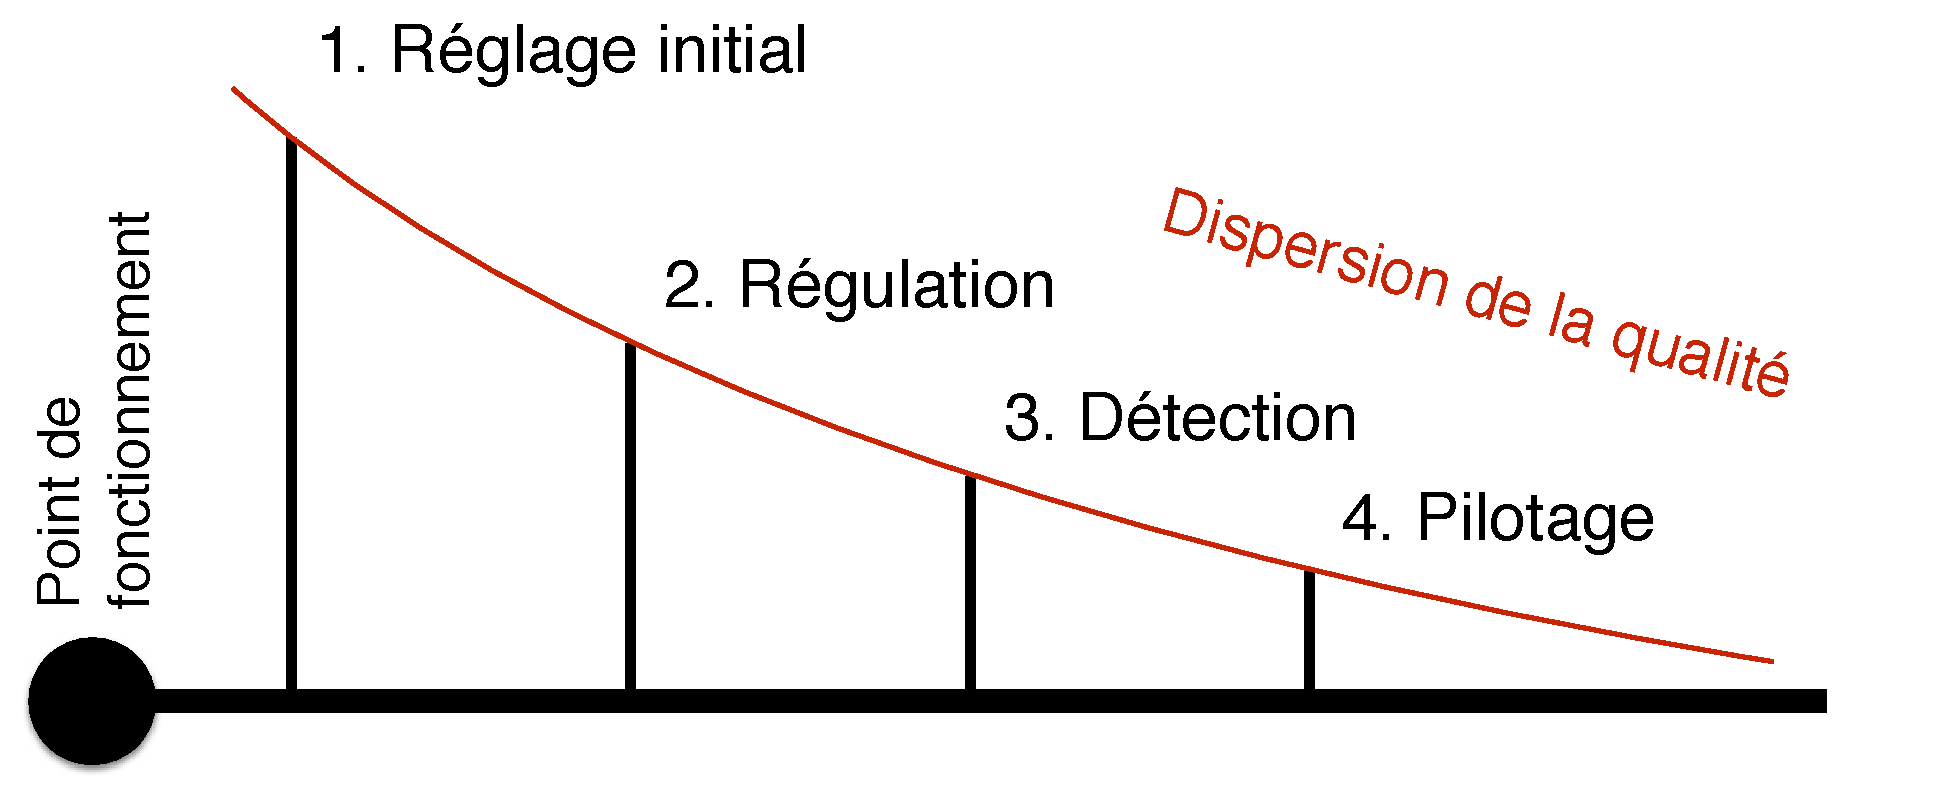
\includegraphics[width=\textwidth,height=\textheight,keepaspectratio]{../Chap1/Figures/Sapristi_EtatArt_Pilotage_en_Injection_Plastique.pdf}
%	\caption{Vers le pilotage du point de fonctionnement du procédé pour optimiser la qualité du produit.}
%	\label{fig:vers_le_pilotage}
%\end{figure}
% La Figure \ref{fig:vers_le_pilotage} récapitule cette démarche.


\section{Pilotage des caractéristiques de la pièce produite}
Le pilotage d’un procédé demande dans un premier temps de détecter les situations hors-contrôles.
Dans le cas où le procédé n'est pas dans sa configuration cible, on mesure l’écart entre la situation hors-contrôle et la situation cible.
Puis on ajuste un ou plusieurs paramètres réglables du procédé, afin de se rapprocher de la situation cible.
Plusieurs stratégies de pilotage ont été proposées dans la littérature.
Certaines utilise une modélisation physique simplifié du procédé, d'autres s'appuient sur une base de connaissance préétablie ou utilisent une analyse statistique.
Ces systèmes reposent sur l’instrumentation de la presse et de l'outillage pour mesurer les conditions appliquées au polymère.
L'évaluation des performances de ces stratégies passe par la mesure de dispersions des caractéristiques des produits.
Dans une démarche pragmatique, le pilotage des caractéristiques du produit peut également se réaliser en mesurant directement les caractéristiques des produits ($\boldsymbol{C_1}$ et $\boldsymbol{C_0}$ Figure \ref{fig:annexe_zigzag}).
% C'est l'objectif du projet FUI SAPRISTI.
Dans le cadre de nos travaux, nous mesurerons la qualité des pièces juste après la sortie de l'outillage ($\boldsymbol{C_1}$).
Notre démarche de mesure est présentée dans le Chapitre \ref{ch:measure}.

En 2001, \citeauthor{nwokah_control_2001} synthétisent les avancées réalisées dans le cadre du pilotage du procédé \cite{nwokah_control_2001}.
Ils définissent deux contraintes principales au développement du pilotage :
\begin{itemize}
	\item la méconnaissance des relations entre les paramètres d’entrées et les caractéristiques finales du produit ($\boldsymbol{P_i}$ et $\boldsymbol{C_i}$ Figure \ref{fig:annexe_zigzag}),
	\item le manque de possibilité d’ajustement des réglages du procédé.
\end{itemize}
Ils argumentent que l’amélioration d’une caractéristique du produit se fera souvent au détriment d’une autre caractéristique, ou bien par l'augmentation des coûts de produit.
Cette contrainte de coût est courante pour les productions industrielles à faible marge.

% \paragraph{Ajustement du procédé à partir des caractéristiques du produit}\mbox{} \\
L’ajustement statistique des procédés (\textit{Statistical Process Adjustement}) est un domaine situé à l’intersection de la régulation automatique et de la Maîtrise Statistique des Procédés.
Ce domaine d'étude étudie les relations entre les paramètres du procédé et les caractéristiques du produit, par une approche statistique.
Un exemple de relations entre les paramètres du procédé d’injection-moulage, qui conditionnent les caractéristiques de la pièce produite, concerne la vitesse d'avance ($\boldsymbol{P_3}$ Figure \ref{fig:annexe_zigzag}).
Celle-ci est liée à la viscosité de la matière ($\boldsymbol{C_3}$) et elle définit le débit d’injection ($\boldsymbol{P_3}$).

Il y a également une influence des paramètres du procédés sur la structure interne de la pièce.
Les travaux de doctorat de \citeauthor{giroud_mesure_2001} étudie l'influence des paramètres du procédé ($\boldsymbol{P_3}$) sur les contraintes internes ($\boldsymbol{C_1}$) \cite{giroud_mesure_2001}.
Le profil de pression appliqué à la pièce pendant la phase d'injection conditionne les contraintes internes résiduelles.
Ces contraintes seront figées dans la pièce par la modification de la forme et de l'orientation des chaînes de polymères.
La relaxation de ces contraintes peut provoquer des déformations géométriques.
C'est une des causes principales du retrait, qui apparait plusieurs heures après la production.

% \citeauthor{del_castillo_statistical_2006} réalise une rétrospective des travaux réalisés dans le domaine de l'Ajustement Statistique des Procédés \cite{del_castillo_statistical_2006}.
% Il identifie les méthodes de modélisation bayésiennes pour l'ajustement optimal des paramètres, comme des pistes privilégiées de recherche.
% Nous présenterons ces méthodes d'optimisations dans le Chapitre \ref{ch:metric_learning} §\ref{subsec:bayesian_opt}.

\subsection{Ajustement du procédé à partir de caractéristiques prédites} \label{parag:adjust_predict}
Il est difficile de mesurer les pièces en sortie de machine.
Les causes sont une durée de mesurage trop longue qui est supérieure au temps de cycle, un coût trop élevé ou simplement une mesure non faisable.
% De plus, le manque de spécifications concernant les caractéristiques de la qualité des pièces n’a pas encouragé l’utilisation de la mesure directe.
Excepté pour le dimensionnel, la notion de qualité dans les cahiers des charges est rarement normalisée.
Elle nécessite l'interprétation humaine, qui est difficile à programmer dans un ordinateur et également à transmettre entre humains.
Le transfert de la notion de qualité de l'expert humain vers le système de contrôle est un des objectifs de notre travail que nous présentons dans le Chapitre \ref{sec:metric_learning}).
C'est pourquoi de nombreux systèmes de la littérature ont choisi de prédire les caractéristiques des pièces produites ($\boldsymbol{C_1}$ Figure \ref{fig:annexe_zigzag}) à partir de variables du procédé ($\boldsymbol{P_i}$).
La prédiction obtenue est ensuite utilisée à des fins d’ajustement des paramètres du procédé pour optimiser les caractéristiques du produit.

En 1993, \citeauthor{haeussler_quality_1993} \cite{haeussler_quality_1993} utilisent un réseau de neurones pour prédire la masse et la longueur des pièces ($\boldsymbol{C_1}$ Figure \ref{fig:annexe_zigzag}), à partir de paramètres du procédé ($\boldsymbol{P_3}$, $\boldsymbol{P_2}$).
% Ils entrainent un réseau 9-21-2 à partir des mesures sur une production de 162 cycles continues.
Le réseau prédit la masse des pièces avec 20\% d'erreur et la longueur avec 11,6\% d'erreur.
Ces résultats sont comparés avec une régression polynomiale d'ordre 3, 25\% d'erreur pour la masse et 21\% d'erreur pour la longueur.
Le réseau de neurones est plus performant que la régression polynomiale d'ordre 3 car c'est une composée de fonctions non-linéaires.
% Cette étude conclut sur la nécessité de l'utilisation d'modèle adaptatif pour un réaliser le pilotage en cycle industriel.
Enfin, les auteurs remarquent que le modèle prédictif doit être enrichit au fur et à mesure des cycles, à partir des nouvelles mesures.
Le modèle ne doit pas se limiter à modéliser un jeu de données statique.
Nous reprenons cette idée dans nos travaux, en proposant un modèle de la notion de qualité qui est enrichit au fur et à mesure de la production §\ref{sec:metric_learning}.

En 1996, \citeauthor{woll_online_1996} proposent d'utiliser un réseau de neurones pour prédire la masse des pièces, à partir des profils de pression mesurées dans l'outillage et dans la buse \cite{woll_online_1996}.
À partir de la prédiction de la masse, la pièce est acceptée ou rebutée si la masse prédite est trop éloignée de la masse cible.
L'écart acceptable à la cible est définie selon la démarche MSP §\ref{parag:spc}.
Le réseau de neurones est appris comme un modèle inverse du procédé.
Les profils de pression sont les variables d'entrées ($\boldsymbol{C_2}$, $\boldsymbol{C_1}$ Figure \ref{fig:annexe_zigzag}) et les variables de sorties sont les consignes de pression de maintien ou de température du fourreau ($\boldsymbol{P_2, P_1}$).
Les paramètres sont ajustés cycle après cycle en comparant le profil de pression courant, avec le profil cible.
% L'analyse MSP est réalisée sur la valeur de pression maximale qui est mesurée dans l'outillage.
Le réseau est entrainé sur un jeu de données issues de simulations, afin d'éviter de réaliser une longue campagne d'essais.
% La convergence du modèle étant observé pour 2000 essais.
L'essai est réalisé pour un unique matériau et la caractéristique cible de la pièce est sa longueur.
% Les résultats montrent la capacité supérieure des réseaux de neurones à prédire les non linéarités comparée à la régression linéaire multiple utilisé par SPC.
% L'exactitude de la prédiction des mesures est augmentée de 10\% et le taux de faux positif est réduit de moitié.
% Le réseau rejette les perturbations.
% L'étude conclue sur la nécessité d'entrainer le réseau sur plusieurs profils dont les températures.
À contrario de cette étude, dans nos travaux, nous avons choisi de mesurer des données réelles sur des machines industrielles.
En effet, notre étude de la littérature montre que les simulations du procédé d'injection-moulage sont limitées.

Dans sa thèse, \citeauthor{chen_study_2002} proposent une méthodologie pour établir le profil de vitesse d’injection optimal ($\boldsymbol{P_3}$ Figure \ref{fig:zigzag}) \cite{chen_study_2002}.
Il modélise également la température du fondu par un second réseau de neurones ($\boldsymbol{P_2}$).
Disposant d'un modèle représentatif, il calcule le profil de température et la pression à imposer pour la phase de plastification, afin d'obtenir un température définie pour la matière qui sort de la buse ($\boldsymbol{C_3}$). 
% Il conclut sur la nécessité de garantir une vitesse de front constante lors de l'injection, afin d’obtenir une qualité produit optimale.

En 2004, dans ces travaux de doctorat, \citeauthor{yang_injection_2004} introduit l'utilisation du contrôle prédictif pour ajuster la vitesse d'avance de la vis lors de l'injection \cite{yang_injection_2004}.
Le contrôleur s'appuie sur l'automatique pour la régulation des procédés industriels (aussi appelée \textit{Global Process Control} ou \textit{Engineering Process Control}) qui consiste à utiliser des régulateurs Proportionnels Intégrateur Dérivateurs pour ajuster les paramètres afin d'obtenir des caractéristiques cibles du produit.
La masse de chaque pièce est prédite à partir des mesures sur le procédé ($\boldsymbol{C_2, C_1}$ Figure \ref{fig:annexe_zigzag}).
À partir de la prédiction, la vitesse d'injection ($\boldsymbol{P_3}$) est ajustée cycle après cycle.
% Un algorithme d'apprentissage itératif en logique floue compense les temps de réponses long des actionneurs.
Ce travail montre la limite que pose l'utilisation des servovalves pour ajuster les paramètres du procédé.
Les servovalves ont un temps de réponse lent, de l'ordre de la seconde.
Ainsi, il est nécessaire d'anticiper la valeur de la consigne.  %, notamment lorsqu'il s'agit d'imposer des consignes temporelles précises.
% À l'aide de l'ensemble des ces techniques, ce travail montre qu'il est possible de détecter les variations de la masse pendant le cycle, sans nécessité une pesée de la pièce.
Ce travail montre qu'il est possible d'ajuster les conditions de maintien et de refroidissement afin de compenser la variation de masse prédite.
L'auteur conclut sur la possibilité de piloter d'autres caractéristiques du produits, en utilisant la même démarche : les géométries et l'aspect des pièces pourraient être ajustés, sous réserve de pouvoir prédire les caractéristiques.

\subsection{Ajustement à partir des caractéristiques mesurées sur le produit}
La section précédentes étudiaient la prédiction des caractéristiques des produits.
Il est également possible de mesurer les caractéristiques du produit.
Dans l'ensemble de la littérature, les caractéristiques mesurées sur les pièces sont limitées à la masse et à quelques cotations géométriques.
L'aspect des pièces n'a jamais été mesurée en cycle.
La masse est la caractéristique la plus mesurée, car la pesée peut facilement être réalisée pendant le cycle d'injection-moulage.
Il suffit de disposer d'un bras robotique préhenseur et d'une balance instrumentée.
Les mesures complémentaires de la qualité des produits sont effectuées après de la production d'un lot, mais non pendant le cycle d'injection.
Il serait intéressant de réaliser une caractérisation complète de la pièce produite, pendant le temps de cycle, afin de pouvoir optimiser les caractéristiques des pièces suivantes, à partir de ces mesures.
La limite à cette démarche est la durée des mesures, qui doit être inférieure au temps de cycle.

En 1998, \citeauthor{fournier_conduite_2006} a proposé un ajustement des paramètres du procédé à partir de la mesure de la masse du produit \cite{fournier_conduite_2006}.
Le matériau qui a été utilisé est le Poly(Téréphtalate de Butylène).
C'est un semi-cristallin sensible aux phénomènes de retrait.
Le système de l'étude utilise un modèle physique simplifié du procédé pour réguler les paramètres en boucle fermé.
% L'écart entre la masse mesurée et la masse cible est ajouté à la boucle de régulation.
Deux perturbations ont été appliquées pendant le cycle : un changement de la matière et un changement de la température dans le fourreau.
Afin de limiter les contraintes internes du matériau, les pièces sont passées par un recuit.
Les mesures des retraits volumiques et de résiliences (chocs Charpy) ont montré une dispersion de masse réduite de 24\% avec l'utilisation du correcteur sur la masse.
La dispersion du retrait volumique, mesurée deux jours après la production des pièces, est réduite de moitié.
Cependant, une cotation géométrique augmente ; elle correspond à l'épaisseur de la pièce.
Après recuit, le retrait volumique est diminué de 12\% par rapport à un procédé non régulé.
La résilience après recuit est quant à elle augmentée de 23\%.
% L'étape de recuit peut être assimilé aux étapes de peintures qu'une pièce est susceptible de subir.
Ces résultats obtenus sont encourageants.
% L'étude montre qu'il y a un intérêt à ajuster les paramètres du procédé en fonction des caractéristiques du produit mesurées dès la sortie de la machine ($\boldsymbol{P_1}$).
% Nos travaux s'inscrivent dans cette démarche.

Une piste de travail importante serait de considérer les caractéristiques des produits finaux ($\boldsymbol{C_0}$ Figure \ref{fig:annexe_zigzag}) pour ajuster le procédé.
Cela nécessitera nécessairement l'utilisation d'un modèle prédictif, car la pièce finale sera obtenue plusieurs heures après son moulage, après son refroidissement.

La même année, \citeauthor{ivester_automatic_1998} ont proposé une méthode d'ajustement à partir de la mesure des caractéristiques \cite{ivester_automatic_1998}.  % qui s'appuie sur un modèle du procédé qui est construit au fur et à mesure de la production,
Les paramètres du procédé sont ajustés par descente de gradient au fur et à mesure de la production (cette méthode est détaillée dans le Chapitre \ref{ch:metric_learning} \ref{parag:neural_networks}).
% Ainsi, le modèle procédé n’est mis à jour que lorsqu’il ne permet plus d’estimer les changements.
L'étude indique que la caractérisation de la qualité des pièces est réalisée par un opérateur humain.
Dans le cadre de nos travaux, nous chercherons à automatiser cette caractérisation.
% Cette méthode d’optimisation des réglages requière que l’opérateur entre les paramètres mesurées ou analyse les mesures dans le cas de caractéristiques d’aspect.
% L’étude conclue sur la viabilité de la méthode et sur l’intérêt d’automatiser la mesure de la qualité des pièces.
Cette méthode est néanmoins dépendante des points de fonctionnement initiaux, qui sont choisis aléatoirement.
C’est pourquoi, \citeauthor{yang_knowledgebased_2000} propose l'ajustement des paramètres du procédé par optimisation d'un modèle qui lie les paramètres avec les caractéristiques du produit, préalablement établi \cite{yang_knowledgebased_2000}.
% C’est un modèle multivarié qui permet de rendre indépendant le système des paramètres initiaux avant optimisation.
Un modèle initial multivarié est définie à partir de la connaissance théorique du procédé.
% C’est ce modèle empirique multivarié qui détermine le point de fonctionnement initial.
% Un algorithme d'apprentissage permet d’optimiser ce modèle pour un produit et une machine.
% L’intérêt du modèle préétablie est de proposer un point de fonctionnement.
% L'apprentissage passe par la comparaison des caractéristiques qualités données par le modèle préétablie et des caractéristiques qualités mesurées sur les pièces.
% Par la suite, le modèle initial est ajusté au fur et à mesure de la production.
Par la suite, les caractéristiques prédites par le modèle sont comparées aux mesures réelles, et les coefficients du modèle sont ajustés pour diminuer l'écart de la prédiction.
% L'étude compare la faisabilité théorique obtenue par simulation et le point de fonctionnement donné par le modèle relationnel KBT, puis le point de fonctionnement obtenu par plan d'expérience central composite.
Une comparaison expérimentale est réalisée entre le système proposé et un point de fonctionnement optimisé à partir de la réalisation d'un plan d'expériences Central Composite (§\ref{parag:doe_cc}).
7 caractéristiques qualités sont mesurées sur le produit.
5 paramètres sont pilotés sur la machine.  % et leurs limites sont connues du modèle.
Le protocole expérimental est détaillé : les 20 premières pièces de chaque essai ne sont pas prises en compte, en attendant la stabilisation du procédé.
Par la suite, 5 pièces sont mesurées 15 à 25 minutes\footnote{
	Nous remarquons que l'amplitude temporelle de 10 minutes est grande.
	En effet, si les pièces sont conservées dans le même atelier de production, alors nous pouvons estimer que leur vitesse de refroidissement est identique.
	Aussi pour une même durée de refroidissement, les caractéristiques seront identiques.
	Or cette durée de refroidissement varie ici beaucoup. 
	Nous recommandons de mesurer les pièces quelques secondes après la sortie du moule, en maitrisant le délai de mesure, afin d'éviter d'introduire une erreur.} après leur sortie du moule pour que leurs caractéristiques géométriques soient également stabilisées.
Les résultats de l'étude montrent que le plan Central Composite n'inclue qu'un petit espace de la plage de réglage du procédé.
Il est alors difficile de trouver un point de fonctionnement optimal à partir du modèle issu du plan d’expérience.
L'étude aurait pû positionner les bornes du plan d'expériences aux limites du procédé.
Le système d'apprentissage proposé dans l'étude est capable de trouver un point de fonctionnement satisfaisant en 10 essais, tandis que le plan Central Composite demande 45 essais.
L'introduction d'un modèle initial issue de la connaissance théorique du procédé permet de diminuer le nombre d'essais à réaliser pour trouver une solution optimale.
% Enfin, nous notons que la mesure des caractéristiques qualités du produit est ici facilité car ce sont des disques DVD.
% Les mesures ont une résolution élevé puisqu'un micromètre laser mesure un profil sur la surface des disques.
% La capabilité du moyen de mesure est excellente.
% Une bonne capabilité du système de mesures est un pré-requis, pour la caractérisation des pièces, et pour le pilotage du procédé.

En 2001, \citeauthor{lau_neural_2001} propose de réaliser un modèle inverse du procédé, à multiples entrées et multiples sorties, par apprentissage d'un réseau de neurones \cite{lau_neural_2001}. % vérifier les capacités de création  d'un modèle multi entrées-sorties du procédé d'injection par réseau de neurones à propagation inverse.
L’objectif est que le réseau suggère des ajustements des paramètres du procédé pour obtenir une pièce cible aux dimensions spécifiées.
Les caractéristiques dimensionnelles portent sur trois longueurs et l'épaisseur de la pièce.
L'apprentissage du réseau est réalisé sur les mesures récoltés sur 100 pièces, en faisant varier sept paramètres du procédé : la température du fourreau centrale et la température de l'arrière du fourreau, la vitesse de fermeture de l’outillage, la vitesse d’avance de la vis, la force de fermeture, la durée d'injection, la durée de refroidissement, la vitesse d'avance de la vis lors de l'injection et la pression d'injection.
% L'étude mentionne que les quatre dimensions étudiées n'ont pas les mêmes valeurs en fonction de la journées de réalisation des essais.  %, malgré la répétition de paramètres identiques, 
% Il ne suffit pas de répéter des paramètres
Les valeurs des dimensions attendues sont appliquées en entrée du modèle.
Ce dernier indique en sortie les valeurs du point de fonctionnement permettant de produire une pièce avec ces dimensions.
La démarche du système est alors d'obtenir l'écart entre les paramètres pour les caractéristiques actuelles et pour les caractéristiques cibles, puis d'ajuster les paramètres en soustrayant ces écarts, afin de compenser les variations des caractéristiques pièces.
En connaissant le réglage utilisé pour produire les pièces, l'étude propose de régler les paramètres dans des proportions inverses afin de compenser les variations de pièces.
Cette démarche suppose que les paramètres sont indépendants, ce qui n'est pas le cas pour le procédé d'injection-moulage.
% Néanmoins, après 3 itérations de réglages successifs, le réseau parvient à converger vers une erreur quadratique moyenne (RMS) de 0,07.
% Ce résultat est comparé à une précédente étude des auteurs [Lau et Wong, 1998] qui utilisait un système hybride à logique floue qui convergeait en 3 itérations vers une erreur quadratique moyenne (RMS) de 0,06.
% La méthode proposée est moins performante qu'un système à logique flou et réseaux de neurones mais plus simple à mettre en œuvre.
% De plus, une optimisation de la topologie du réseau de neurones, telle que la recherche en informatique la permet aujourd'hui améliorerait ce résultat.

Récemment, en 2015, \cite{johnston_-line_2015} réalise une étude à l'aide d'un plan d'expériences à quinze essais pour douze facteurs, pendant 30 minutes de production par essais, totalisant 942 cycles d'injection-moulage, soit 60 pièces par essais.
% Il dérive des fonctions de transfert et des composantes principales pour chacune des 46 sorties du procédé.
Pour chaque cycle, une boucle d'optimisation évalue et minimise l'écart à une dimension géométrique cible par un ajustement des paramètres du procédés ($\boldsymbol{P_1, P_2, P_3}$ Figure \ref{fig:annexe_zigzag}).
% Le contrôleur qui est proposé est capable de détecter les variations du procédé par comparaison avec un modèle de référence préétabli.
% Le contrôleur ajuste alors les paramètres pour atteindre le modèle de référence.
Un objectif de réduction du temps de cycle est ajouté grâce à une pénalité temporelle dans la fonction à minimiser.
Un double objectif est atteint : le temps de cycle est réduit et la variabilité des dimensions des pièces est réduite.
L'étude conclut qu’une optimisation  multi-paramètres, par exemple sur les caractéristiques dimensionnelles, est possible.
Les auteurs mettent en valeur l'intérêt de leur méthode par rapport à un ajustement manuel des paramètres du procédé.
Leur système permet de réduire le nombre d'essais à réaliser pour régler le procédé d'un facteur dix.




\FloatBarrier
\chapter{Économie du secteur de la plasturgie française}
\label{Ann:2}

Le Tableau \ref{fig:molding_economy} présente la répartition économique industrielle française par secteurs d'activité.
Elle indique une marge moyenne de 27\% pour le secteur de la plasturgie française, en 2016 \cite{directiongeneraledesentreprises_chiffres_2019}.
Le chiffre d'affaire moyen par entreprise est de 1,3 millions d'euros en 2016.

\begin{figure}[hbt]
	\centering
	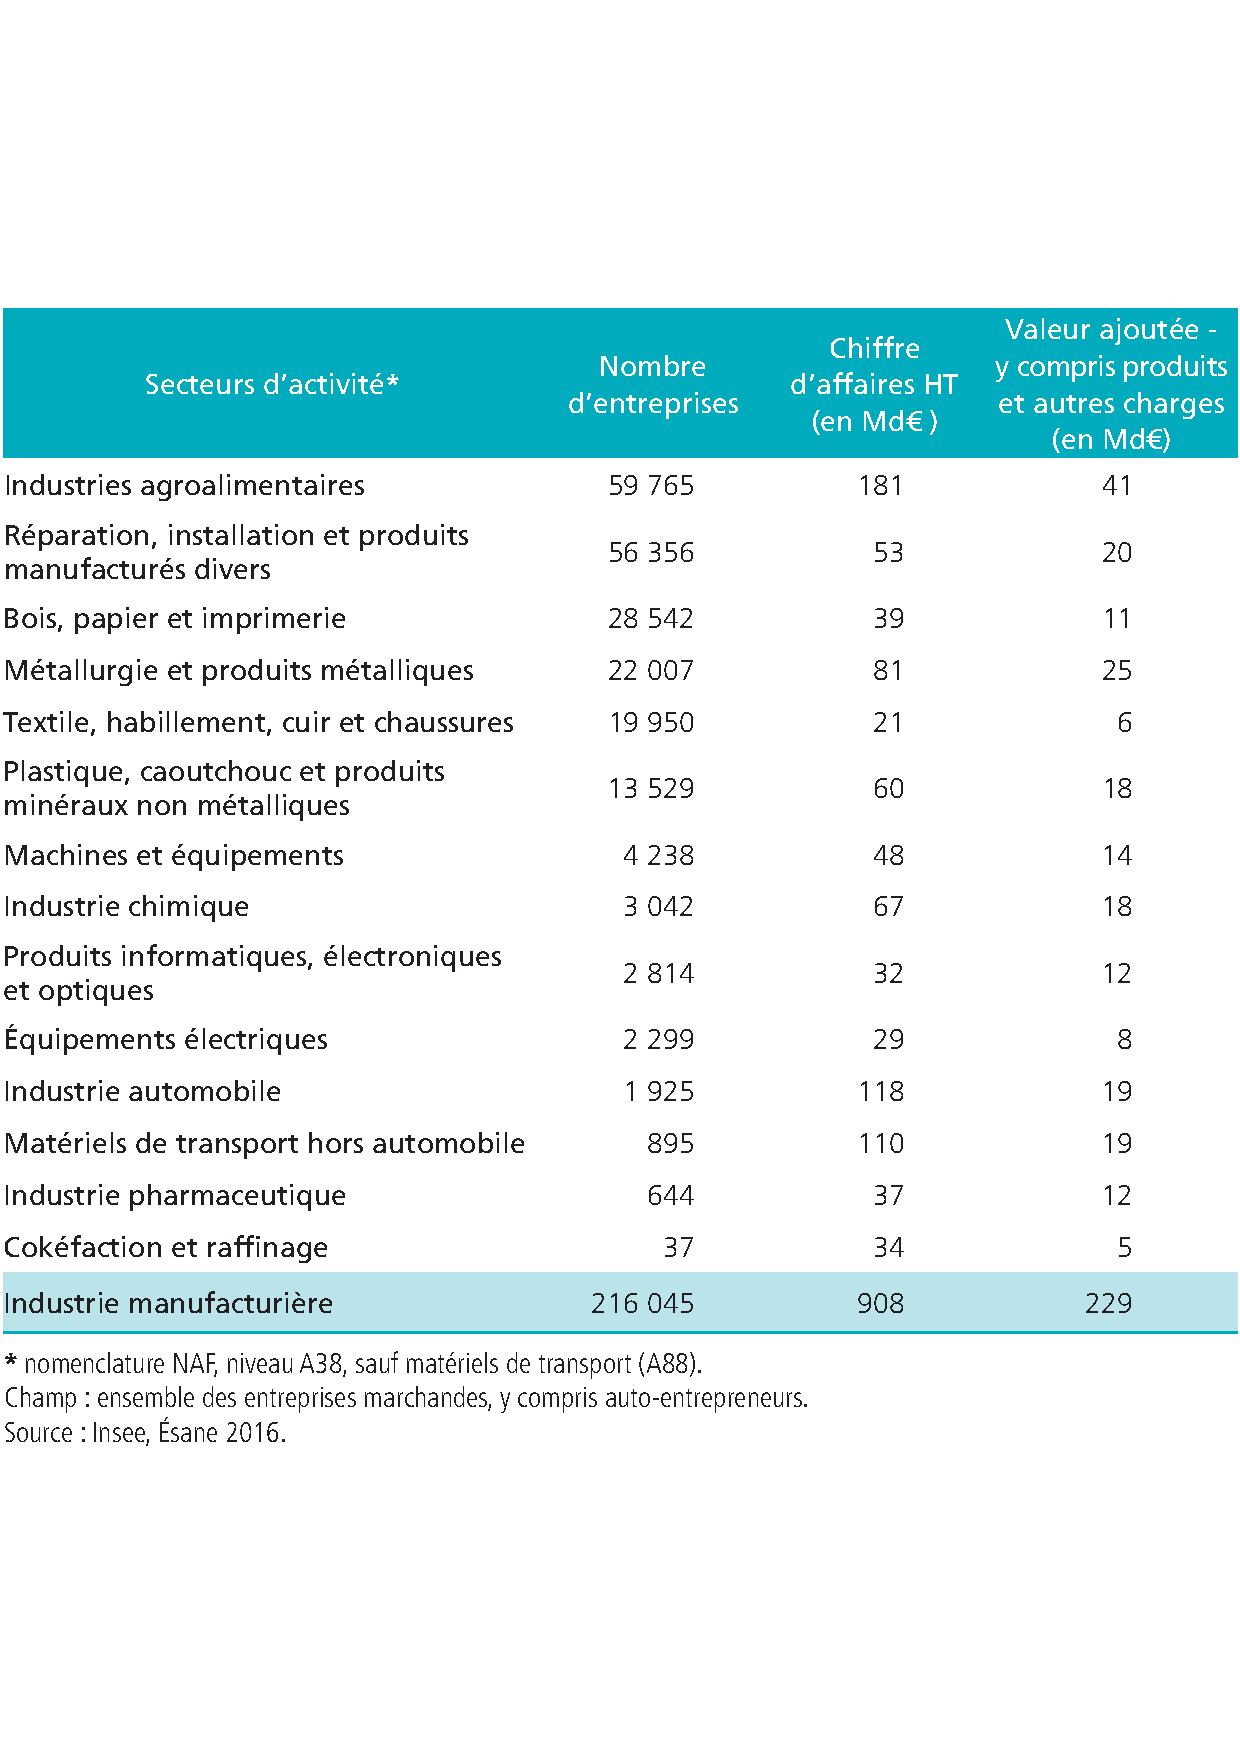
\includegraphics[width=0.85\textwidth,height=\textheight,keepaspectratio]{../Chap1/Figures/2018-Chiffres-cles-industrie-manufacturiere-secteur.pdf}
	\caption{Figure issue du rapport annuel de la \citeauthor{directiongeneraledesentreprises_chiffres_2019} :  \citetitle{directiongeneraledesentreprises_chiffres_2019} \cite{directiongeneraledesentreprises_chiffres_2019}}
	\label{fig:molding_economy}
\end{figure}


\FloatBarrier
\chapter{Apprentissage statistique}
\label{Ann:3}

%==============================================================================	Résumé du chapitre

\begin{center}
	\rule{0.7\linewidth}{.5pt}
	\begin{minipage}{0.7\linewidth}
		\smallskip
		
		\textit{
			Cette annexe propose une synthèse de la théorie de l'apprentissage statistique et une présentation des principaux algorithmes traditionnels.
		}
		
		%\smallskip
	\end{minipage}
	\smallskip
	\rule{0.7\linewidth}{.5pt}
\end{center}

%\adjustmtc
% \minitoc
% \newpage
\bigskip

Cette annexe est complémentaire de la Section \ref{sec:metric_learning}.
Nous présentons la problématique de la performance d'un classifieur, puis les principaux algorithmes d'apprentissage statistique traditionnels.
Dans ce travail de doctorat, nous nous sommes intéressés en particulier aux méthodes de \textit{Deep Learning}, voir la Section \ref{sec:metric_learning}.

\section{Métrique de performances d'un classifieur}
Pour exprimer la performance d'un classifieur, de nombreuses métriques ont été proposées dans la littérature.
Une métrique rend compte de l'écart entre la réponse donnée par un classifieur et la vérité.
La métrique la plus couramment employée est la justesse définie par \citeauthor{metz_basic_1978} \cite{metz_basic_1978}, Équation \ref{eq:accuracy}.
Cette métrique est adaptée au cas où de multiples classes $j$ sont présentes dans le problème.
Nous rapporterons ici toutes les métriques sur le nombre d'échantillons total.
\begin{equation} \label{eq:accuracy}
\text{justesse}(y, \hat{y})=\frac{1}{n_{\mathrm{\acute{e}chantillons}}} \sum_{i=0}^{n_{\mathrm{\acute{e}chantillons}}-1} 1\left(\hat{y}_{j}=y_{j}\right)
\end{equation}

Le procédé d'injection-moulage des thermoplastiques est stable.
Lorsqu'un point de fonctionnement satisfaisant pour obtenir une pièce de bonne qualité est obtenu.
La dérive du procédé au cours du temps est de l'ordre de la journée.
Ainsi, peu de pièces mauvaises sont produites.
C'est pourquoi une population traditionnelle de pièce moulées comportera peu d'individus de mauvaise qualité et une majorité d'individus de bonne qualité.
Ainsi, le choix de la métrique d'évaluation des performances doit tenir compte de la répartition non égalitaire des classes dans l'échantillon.
La justesse ne prend pas en compte les répartitions inégalitaires de classes dans la population, c'est pourquoi ce n'est pas une métrique adaptée à notre problème \cite{japkowicz_class_2002}.

\subsection{Justesse équilibrée}\mbox{} \\
La justesse équilibrée, Équation \ref{eq:balanced_accuracy}, est une métrique qui tient compte de ce problème en intégrant une matrice de poids $\mathbf{W}$ qui compense les déséquilibres inter-classes \cite{brodersen_balanced_2010, mosley_balanced_2013}.
Dans le cas où la répartition des classes est équilibrée, la justesse équilibrée est égale à la justesse.

\begin{equation} \label{eq:balanced_accuracy}
\begin{split}
\text{justesse}_{\text{éq}}(y, \hat{y}, \mathbf{W})=\frac{1}{\sum \hat{\mathbf{w}}_{i}} \sum_{i} 1\left(\hat{y}_{i}=y_{i}\right) \hat{\mathbf{w}}_{i}
\\
\text{avec } \hat{\mathbf{w}}_{i}=\frac{\mathbf{w}_{i}}{\sum_{j} 1\left(y_{j}=y_{i}\right) >_{j}}
\end{split}
\end{equation}

\subsection{Matrice de confusion}\mbox{} \\
Dans notre cas industriel, il est crucial de limiter le nombre de faux positifs, c'est à dire le nombre de pièces mauvaises détectées comme bonnes.
A contrario, les faux négatifs correspondent aux pièces bonnes détectées comme mauvaises.
Sur des pièces moulées en plastique dont le coût de revient est faible, les faux négatifs ne sont pas aussi critiques que les faux positifs pour notre problématique industrielle car la relation client entre en jeu.
En effet, les taux de pièces mauvaises acceptés dans les lots par le client sont, pour les plus drastiques des cahiers des charges, de 5 pièces défectueuses par millions.
Dans ce cas, il vaudra mieux jeter des pièces bonnes que prendre le risque d'envoyer un lot contenant des pièces mauvaises.
Si le coût de revient des pièces est élevé, alors faux positifs et faux négatifs sont à limiter : c'est le zéro défaut.
Si la dimension écologique est prise en compte, on cherchera également à atteindre le zéro défaut : jeter des pièces bonnes est une hérésie écologique, qui plus est : produire des pièces mauvaises.

La littérature présente les nombres de faux positifs et faux négatifs sous la forme d'un Tableau \ref{tab:confusion_matrix}, la matrice de confusion.

% Please add the following required packages to your document preamble:
% \usepackage{multirow}
\begin{table}[]
	\centering
	\arrayrulecolor{black}\begin{tabular}{l|l|l|}
		\cline{2-3}
		& \multicolumn{2}{l|}{Classes vraies}               \\ \hline
		\multicolumn{1}{|l|}{\multirow{2}{*}{Classes prédites}} & Vrais positifs (VP) & Faux Positifs (FP)  \\ \cline{2-3} 
		\multicolumn{1}{|l|}{}                            & Faux négatifs (FN)  & Vrais Négatifs (VN) \\ \hline
	\end{tabular}
	\caption{Matrice de confusion.}
	\label{tab:confusion_matrix}
\end{table}

\subsection{Précision et rappel}\mbox{} \\
La précision et le rappel sont définis à partir de ces valeurs, Équations \ref{eq:precision_recall}.
Elles renseignent sur la pertinence des résultats.

\begin{equation} \label{eq:precision_recall}
\begin{split}
pr\acute{e}cision = \frac{|y \cap \hat{y}|}{|y|} = \frac{\text{VP}}{\text{VP}+\text{FP}}
\\
rappel = \frac{|y \cap \hat{y}|}{|\hat{y}|} = \frac{\text{VP}}{\text{VP}+\text{FN}}
\end{split}
\end{equation}

\subsection{F-mesure}\mbox{} \\
La moyenne harmonique de la précision et du rappel est appelé F-mesure.
Le facteur $\beta$ permet d'ajuster le rapport entre précision et rappel.
Lorsque $\beta = 1$, précision et rappel sont également pondérés, on parle alors de F1-mesure.

\begin{equation} \label{eq:f1_score}
\begin{split}
F_{\beta}=\left(1+\beta^{2}\right) \frac{pr\acute{e}cision \cdot rappel}{\beta^{2} pr\acute{e}cision + rappel}
\\
F_{1}= 2 \frac{pr\acute{e}cision \cdot rappel}{pr\acute{e}cision + rappel}
\end{split}
\end{equation}

L'ensemble de ces métriques est généralisable par moyennage, dans le cas où plus de deux classes existent dans la population :
\begin{itemize}
	\item micro-moyenne : les métriques sont calculées d'après les Équations combinatoires \ref{eq:precision_recall}.
	\item macro-moyenne : les métriques sont calculées pour chaque classes, puis moyennées par l'ensemble des classes.
\end{itemize}

\subsection{Courbe ROC}\mbox{} \\
La courbe ROC (\textit{Receiver Operating Characteristic}) représente la caractéristique de performance d'un classifieur.
Elle a été proposée en 1940 pour distinguer les vrais positifs du bruit de fond sur les relevés radars.
La courbe compare sensibilité (taux de vrais positifs) et spécificité (taux de vrais négatifs) d'un classifieur.
La performance est comparée à la réponse d'un classifieur aléatoire.
Cette courbe peut servir à choisir la valeur optimale de séparation entre deux classes.
Dans notre cas, une valeur milieu, non biaisée est satisfaisante.
La courbe \ref{fig:roc} est issue du meilleur classifieur de la qualité obtenue.
L'écart-type est calculé par validation croisée, §\ref{subsubsec:cross_val}.

\begin{figure}[hbtp]
	\centering
	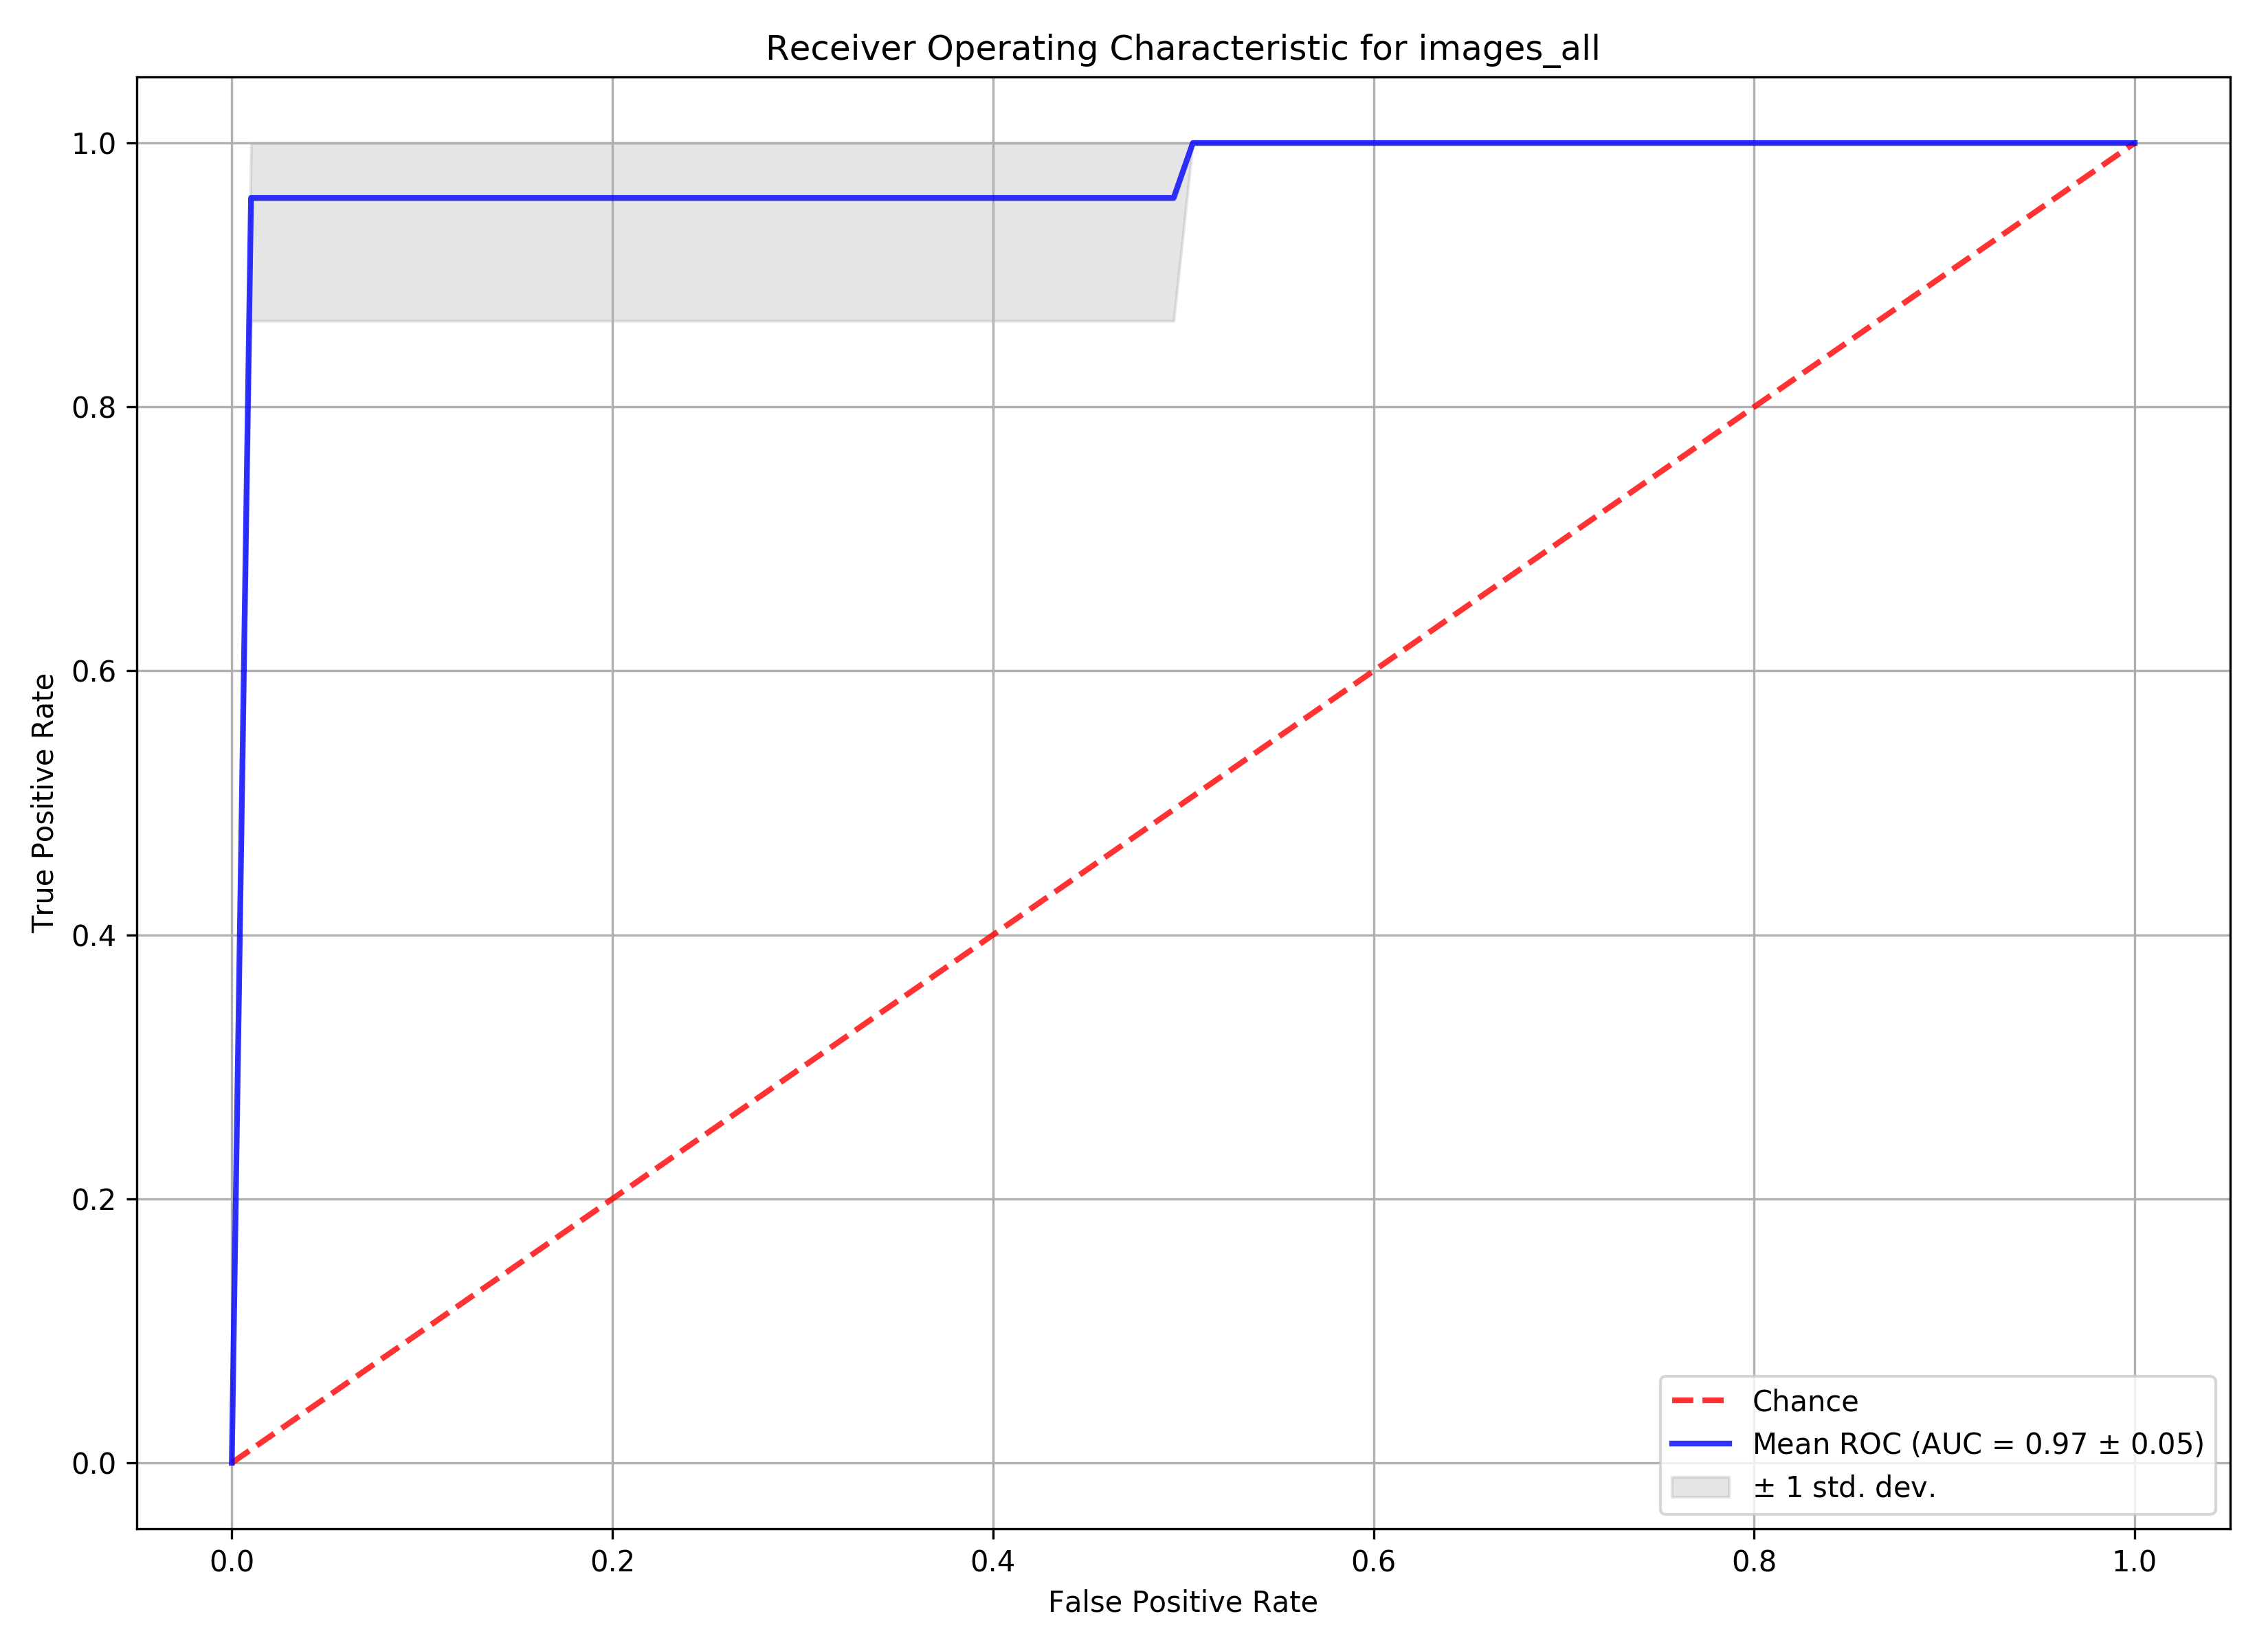
\includegraphics[width=\textwidth,height=\textheight,keepaspectratio]{../Chap4/Figures/roc_images_all_224_3cams_densenet_conv4_PCA20.png}
	\caption{Courbe ROC du meilleur classifieur de la qualité des pièces.}
	\label{fig:roc}
\end{figure}

%TODO AUC : Area Under Curve
% Pour chaque seuil, nous avions des métriques qui résumaient la performance de notre classifieur. Nous allons désormais utiliser une métrique géométrique définie par l’aire sous la courbe. Mais quelle courbe ? Plusieurs possibilités s’offrent à nous :

\subsection{Validation croisée pour la comparaison des performances de classifieurs} \label{subsubsec:cross_val}
Pour comparer les performances de classifieurs, nous comparons la valeur des métriques définies précédemment.
Les classifieurs sont appris sur un jeu de données d'apprentissage et la performance est mesurée sur un jeu de données de test, qui n'a pas été utilisé lors de l'apprentissage.
On réserve traditionnellement 20 pour-cent du jeu de données pour le test.
Une limite de cette méthode est le biais potentiel des deux portions.
Dans le cas de grands jeux de données ($> 2 000$ par classes), le biais est naturellement limité par la variabilité des données.
Dans le cas de jeu de données de plus petites dimensions, il est nécessaire de limiter ce biais.
On utilise des méthodes de validations croisées.
Il s'agit d'entrainer de multiples modèles sur des portions différentes des données, puis d'observer la moyenne et l'écart-type des performances.
Nous présenterons ici la méthode des K-partitions stratifiées par classes (\textit{Stratified K-Folds}), utilisée dans nos travaux.
D'autres méthodes existent mais nous retenons cette dernière par sa robustesse au jeu de données où les classes ne sont pas égales.
Cette méthode est également extensible aux problèmes à classes multiples.
La stratification consiste à associer dans chaque partition une proportion d'échantillons de chaque classe équivalente.
\citeauthor{kohavi_study_1995} conclue ainsi sur l'intérêt de la stratification, en matière de réduction du biais des modèles \cite{kohavi_study_1995}.
Le nombre de partition $k$ est choisi en fonction du nombre d'échantillons disponible.
Dans nos problèmes où les jeux de données sont inférieurs à mille échantillons, nous fixons $k=3$.
Dans nos travaux, nous utiliserons l'implémentation de la librairie \textit{Scikit-Learn} \cite{pedregosa_scikit-learn_2011}.
La Figure \ref{fig:StratifiedKFold} représente l'effet de cette méthode sur un jeu de données.

\begin{figure}[hbtp]
	\centering
	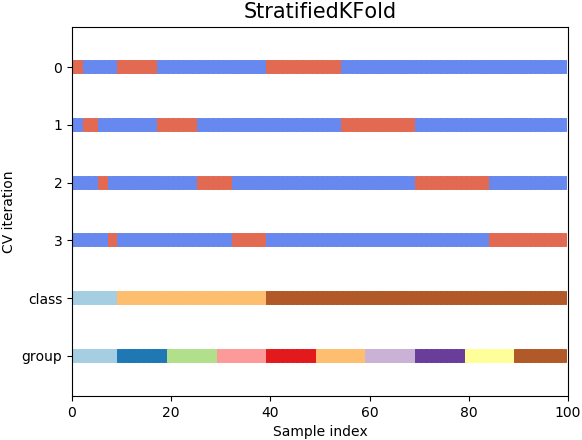
\includegraphics[width=0.7\textwidth,height=0.7\textheight,keepaspectratio]{../Chap4/Figures/sphx_glr_plot_cv_indices_003.png}
	\caption{\emph{Stratified 4-Folds}. Figure extraite de la \href{https://scikit-learn.org/stable/auto_examples/model_selection/plot_cv_indices.html}{doc \textit{SciKit-Learn}, License BSD 3-clauses}.}
	\label{fig:StratifiedKFold}
\end{figure}

Lorsque l'on souhaite réaliser un optimisation du classifieur en lui-même (hyper-paramètres), une partition de données de validation est introduite.
Chaque classifieur sera entrainé sur le jeu d'apprentissage, puis validé sur le jeu de validation.
Enfin, le meilleur classifieur obtenu sera évalué sur le jeu de test, qui n'aura jamais été utilisé ni pendant l'apprentissage, ni pendant l'optimisation.
Dans ce cas, le jeu de données est découpé en trois portions présentées dans le Tableau \ref{tab:cross_val}.
Nous emploierons cette répartition dans l'ensemble de nos travaux.

%\newcolumntype{x}[1]{>{\centering\let\newline\\\arraybackslash\hspace{0pt}}p{#1}}
\newcolumntype{C}[1]{>{\centering\arraybackslash}p{#1}}
\begin{table}[]
	\centering
	\begin{tabular}{| C{8.1cm} | C{2.7cm} | C{2.7cm} |}
		\hline
		Apprentissage & Validation & Test \\ \hline\hline
		60\% & 20\% & 20\% \\ \hline
		Apprentissage du modèle & Validation du modèle & Validation du meilleur modèle \\ \hline
	\end{tabular}
	\caption{Répartition du jeu de données : apprentissage, validation et test.}
	\label{tab:cross_val}
\end{table}

\section{Apprentissage statistique traditionnel}
Nous présenterons dans cette section les méthodes de classification les plus utilisées dans la littérature.
Dans ce travail, nous discuterons de l'intérêt de ces différents classifieurs sur notre application industrielle.
La méthode des k-plus-proches voisins est la plus utilisée sur des problèmes de vision par ordinateur.
Nous distinguons les classifieurs dits "traditionnels", des classifieurs \textit{Deep Learning} qui utilisent des réseaux de neurones profonds : leur spécificité est de synthétiser dans un seul modèle la méthode d'extraction de l'information et la classification.
Ces derniers seront présentés et discutés dans la Section \ref{subsubsec:deep_learning}.

\subsection{Machine à vecteurs de support}\mbox{\label{parag:svm}} \\
Soit les couples d'échantillons et leurs annotations de classe binaire associées $(\mathbf{x}_i, y_i)$.
\citeauthor{vapnik_patterns_1963} \cite{vapnik_patterns_1963} proposent une solution au problème de classification binaire dans un espace à grandes dimensions, permettant de prédire l'annotation $y_i$ à partir des données $\mathbf{x}_i$.
Une machine à vecteurs de support (\textit{Support Vector Machine}) cherche à trouver l'hyperplan qui sépare au mieux les deux classes (Figure \ref{fig:svm}). $\vec{\mathbf{w}}$  est orthogonal à l'hyperplan.
L'hyperplan est choisi tel que la distance $b$ entre le plan et les échantillons de $\mathbf{x}_i \in \mathbf{X}$ les plus proches de ce dernier, soit maximale : c'est la recherche de la marge maximale $\frac{b}{\|\vec{\mathbf{w}}\|}$.
L'hyperplan obtenu est alors défini par ses vecteurs supports $\mathbf{x}_i$.
\citeauthor{cortes_supportvector_1995} proposent l'utilisation d'une fonction de marge dite \textit{soft} basée sur le coût de \textit{hinge} \cite{cortes_supportvector_1995, vapnik_support_1997}.
Ils introduisent un terme de régularisation $C$. Trouver le classifieur optimal revient alors à la résolution du problème d'optimisation de l'Équation \ref{eq:svm}.

\begin{equation} \label{eq:svm}
\begin{split}
f_{SVM}(\mathbf{x}_i, y_i) = \arg \min \left[\frac{1}{n} \sum_{i=1}^{n} \max \left(0, 1-y_{i}\left(\vec{\mathbf{w}} \cdot \vec{\mathbf{x}}_{i}-b\right)\right)\right]+ C \|\vec{\mathbf{w}}\|^{2}
\\
\text{avec } \mathcal{L}_{Hinge}(\mathbf{x}_i-b, y_i) = \max (0, 1 - y_i \cdot (\mathbf{x}_i-b))
\end{split}
\end{equation}

Lorsque les échantillons ne sont pas linéairement séparables, \citeauthor{boser_training_1992} \cite{boser_training_1992} proposent d'effectuer une transformation $\varphi$ de l'espace des données, afin de trouver un espace où les échantillons sont linéairement séparables.
La transformation $\varphi$ a pour noyau une forme choisie (c'est le \textit{kernel trick}, proposé par \citeauthor{aizerman_theoretical_1964} \cite{aizerman_theoretical_1964}).
Soit $\mathbf{c}$ et $\varphi$ tel que $\vec{\mathbf{w}}=\sum_{i=1}^{n} \cdot c_{i} \cdot y_{i} \cdot \varphi\left(\vec{\mathbf{x}}_{i}\right)$, on a le noyau $K\left(X, X^{\prime}\right) = \varphi \left(X\right) \cdot \varphi\left(X^{\prime}\right)$.
Cette démarche de transformation vectorielle est utilisée dans de nombreux autres algorithmes.
Les noyaux non linéaires les plus employés sont les noyaux polynomiaux et les noyaux gaussiens de bases radiales (\textit{Radial Basis Function}), Équations \ref{eq:kernels}.
En utilisant le \textit{kernel trick}, un classifieur SVM est alors formalisé par l'Équation \ref{eq:svm_trick}.

\begin{equation} \label{eq:kernels}
\begin{split}
K_{polyn\hat{o}mial}\left(X, X^{\prime}\right) = \left(X \cdot ^{\prime} X + c\right)^{d}, \text{ avec } d \text{ le degré et } c \text{ une constante}.
\\
K_{RFB}\left(X, X^{\prime}\right) = \exp \left(-\frac{\left\|X-X^{\prime}\right\|^{2}}{2 \sigma^{2}}\right) = \exp \left(-\gamma\left\|X-X^{\prime}\right\|^{2}\right), \text{ avec } \gamma > 0
\end{split}
\end{equation}

\begin{equation} \label{eq:svm_trick}
f_{SVM,RBF}(X_i, y_i) = \arg \min \left[\frac{1}{n} \sum_{i=1}^{n} \max \left(0, 1-y_{i}\left(\vec{\mathbf{w}} \cdot \varphi(\vec{\mathbf{x}}_{i})-b\right)\right)\right]+ C \|\vec{\mathbf{w}} \cdot \varphi \|^{2}
\end{equation}

Le choix des hyper-paramètres $C$ et $\gamma$ est critique pour obtenir de bonnes performances en matière de justesse et de durée de calcul.
$C$ influence la largeur de la marge entre les deux classes.
Ce facteur régularise le classifieur et permet sa généralisation à de nouveaux échantillons.
$C$ est un facteur qui équilibre la nécessité de trouver l'hyperplan le plus simple possible, et le droit aux erreurs de classifications.
Une petite valeur de $C$ encouragera une marge large, ce qui produira un hyperplan simple, mais acceptera des erreurs de classifications.
Enfin, $\gamma$ pondère l'influence d'un unique échantillon sur l'hyperplan.

\begin{figure}[hbtp]
	\centering
	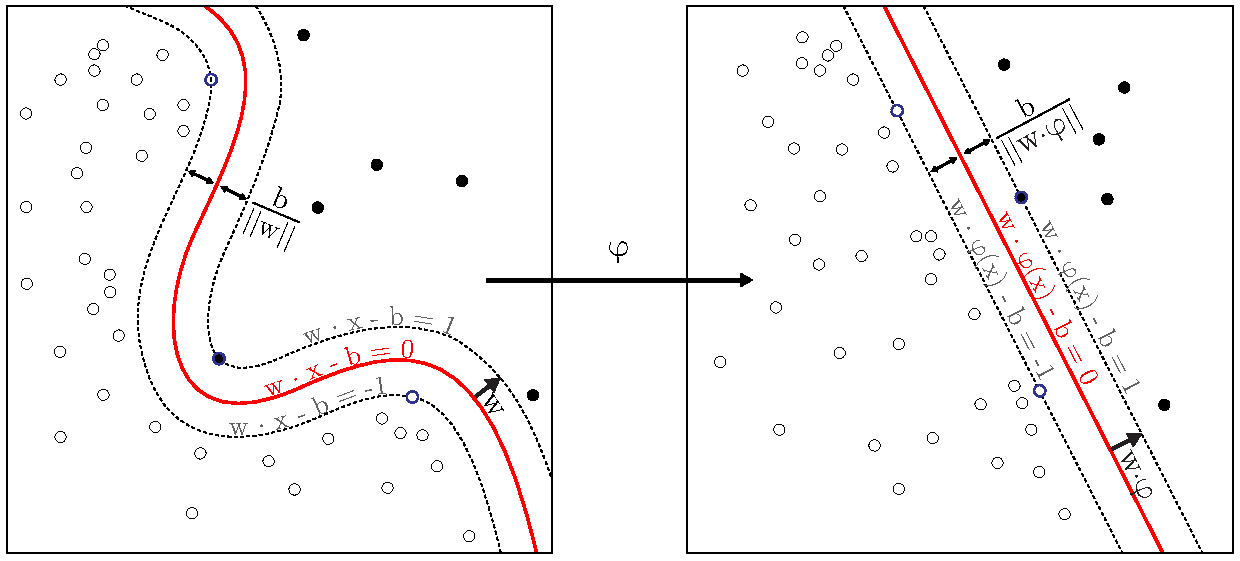
\includegraphics[width=\textwidth,height=\textheight,keepaspectratio]{../Chap4/Figures/Kernel_Machine_Pierre.pdf}
	\caption{SVM avec \emph{kernel trick} $\varphi$. Figure originale de \href{https://commons.wikimedia.org/wiki/File:Kernel_Machine.png}{Alisneaky \ccLogo \ \textnormal{0}, Wikimedia Commons}.}
	\label{fig:svm}
\end{figure}

La librairie \textit{LIBSVM} \cite{chang_libsvm_2011} permet de résoudre le problème avec différents noyaux non linéaires, dans un ordre de grandeur de $\bigO(N^2)$ à $\bigO(N^3)$.
Aussi, elle n'est plus utilisable lorsque le nombre d'échantillon dépasse dix mille.
Dans nos travaux, nous utilisons la librairie \textit{LIBLINEAR} de \citeauthor{fan_liblinear_2008} \cite{fan_liblinear_2008}, au travers de l'interface de la libraire \textit{SciKit-Learn} de \citeauthor{pedregosa_scikit-learn_2011} \cite{pedregosa_scikit-learn_2011}.
La complexité de l'apprentissage, avec des noyaux linéaires, est de l'ordre de $\bigO(N)$, avec $N$ le nombre d'échantillons ce qui rend cette méthode intégrable sur des systèmes embarqués modernes aux vues des puissances de calculs aujourd'hui disponibles.
L'apprentissage d'un modèle peut être effectué pendant le cycle de production et le système de calcul peut être intégré directement au cœur de l'atelier de production, au plus près du procédé d'injection-moulage.

\subsection{K-plus-proches voisins} \mbox{} \label{parag:knn} \\
La méthode des k-plus-proches voisins a été proposée par \citeauthor{fix_discriminatory_1951} \cite{fix_discriminatory_1951} et développée par \citeauthor{cover_nearest_1967} \cite{cover_nearest_1967}.
Cette méthode est à l'origine de méthodes d'apprentissages non supervisées, par exemple celles basées sur les variétés et l'analyse spectrale.
Cette méthode ne cherche pas à construire de modèle générique au problème de classification.
Elle enregistre les positions des échantillons du jeu d'apprentissage dans l'espace des données.
La classification d'un nouvel échantillon est la classe majoritaire sur l'ensemble des échantillons parmi les $k$ plus proches voisins.
Le nombre de voisins $k$ peut être prédéfini ou bien varier à partir de la densité  de points (la métrique de distance entre points est souvent la norme Euclidienne $\ell_{2}$).
Cette méthode est particulièrement efficace lorsque la séparation entre les échantillons est irrégulière.

%\paragraph{Régression logistique}\mbox{} \\
%TODO

\subsection{Bagging}\mbox{\label{parag:bagging}} \\
Le \textit{bagging} (\textit{\emph{B}ootstrap \emph{agg}regat\emph{ing}}) est une méthode d'association ensembliste de modèles simples afin d'obtenir un méta-modèle aux performances supérieures.
Il est défini par \citeauthor{breiman_bagging_1996} \cite{breiman_bagging_1996}.
La technique permet de limiter le sur-apprentissage.
Pour un jeu de données $\mathbf{X}$ de taille $n$, on génère $b$ lots $\mathbf{X}_b \in \mathbf{X}$ contenant $\sim 10 < m < n$ échantillons tirés aléatoirement selon une distribution uniforme.
Les échantillons, uniques dans $X$, peuvent être répétés dans $\mathbf{X}_b$.
Pour chaque lot $b$, un modèle de l'algorithme choisi est entrainé.
La prédiction du méta-modèle final est la moyenne (ou le vote pondéré) de tous les modèles $f_b$, Équation \ref{eq:bagging}.
Cette méthode d'agrégation de modèles est efficace pour limiter le sur-apprentissage.
La méthode est employée dans les \textit{Random Forests} et elle est souvent combinée avec le \textit{boosting} \ref{parag:boosting}.
La méthode de référence pour calculer le nombre optimal $b$ de fonctions est la sélection du meilleur score par validation croisée \ref{subsubsec:cross_val}.

Une métrique intéressante se base sur la performance individuelle de chaque modèle $f_b$ vis à vis de son jeu de données partiel $\mathbf{X}_b$.
\citeauthor{breiman_bagging_1996} \cite{breiman_bagging_1996} définit l'erreur \textit{Out-of-Bag} comme la moyenne, de l'erreur de prédiction pour chaque échantillon $\mathbf{x}_{i,\bar{b}}$, des modèles $f_b$ avec $ \mathbf{x}_{\bar{b}} \notin \mathbf{X}_b$ qui n'ont pas été entrainés avec les échantillons $x_i$.
Cette erreur est similaire à une erreur de prédiction qui serait calculée sur des échantillons de validation.
Elle permet ainsi de se passer de jeu de données de validation.
Elle est utilisé par les \textit{Random Forests} \ref{parag:random_forests} pour mesurer l'influence des variables sur la prédiction.

\begin{equation} \label{eq:bagging}
f_{boosted} = \frac{1}{b} \sum_{b=1}^{b} f_{b}\left(x_b\right)
\end{equation}

\subsection{Forêt d'arbres décisionnels}\mbox{\label{parag:random_forests}} \\
L'arbre décisionnel est une méthode de classification adaptée au grands jeux de données.
Un arbre se compose de branches avec entre chacune d'elle un nœud.
Chaque nœud répond à une condition sur une variable d'entrée.
Ainsi, le modèle obtenu peut être facilement interprété par l'humain.
Le modèle obtenu est cependant peu robuste aux perturbations des variables d'entrée.
La complexité du modèle est souvent égale au nombre de variables d'entrée ce qui est une cause de sur-apprentissage.
Son utilisation pour des échantillons d'entrée qui comporte une dimension supérieure à dix mille est difficile (par exemple les pixels d'une image).
C'est pourquoi \citeauthor{ho_random_1995}
\cite{ho_random_1995, ho_random_1998} propose un modèle comportant de multiples arbres de décisions (une forêt), chacun entrainés sur une unique partie des variables des échantillons.
La prédiction du modèle est donnée par la moyenne des prédictions de l'ensemble des arbres. 
\citeauthor{breiman_random_2001} \cite{breiman_random_2001} fait évolué la méthode : les arbres sont choisis pour ne pas être corrélés entre eux et leurs sorties sont agrégées par \textit{bagging} \ref{parag:bagging}.

Une utilité indirecte de la notion stochastique des forêts d'arbres décisionnels est la possibilité de mesurer l'influence des variables sur le modèle.
Lors de l'entrainement, l'erreur \textit{Out-of-Bag} \ref{parag:bagging} (équivalente à une erreur de prédiction sur un échantillon de validation) est moyennée pour l'ensemble des arbres.
C'est l'erreur \textit{Out-of-Bag} de référence, pour chacune des variables $j$, $e_{ref, j}$.
À chaque itération, on permute aléatoirement la position des variables $v$ dans le jeu de données et on calcule à nouveau l'erreur \textit{Out-of-Bag}.
Les permutations sont réalisées un grand nombre de fois ($p > 1000$).
On obtient l'importance de la $j^{\text{ième}}$ variable en calculant la moyenne de l'erreur sur toutes les permutations $\bar{e_{perm}}$ de la différence avec l'erreur de référence de la variable : $importance_{j} = \bar{e_{perm, j}} - e_{ref, j}$.
Il est enfin possible de normaliser la valeur de l'importance par l'écart-type sur l'ensemble des variables pour classer les variables sur une échelle continue $[0 ; 1]$.
Nous utiliserons cette méthode pour sélectionner les variables pertinentes.

\subsection{Boosting}\mbox{\label{parag:boosting}} \\
\citeauthor{kearns_thoughts_1988} \cite{kearns_thoughts_1988} pose l'hypothèse de l'existence d'un méta-classifieur qui utiliserait une association de classifieurs aux performances non optimales (légèrement supérieure à une réponse aléatoire) pour obtenir de bonnes performances : le \textit{boosting}.
Dans un tel ensemble, chaque classifieur est ainsi faiblement corrélé avec la totalité des données.
\citeauthor{schapire_strength_1990} \cite{schapire_strength_1990} vérifie l'hypothèse et par la suite \citeauthor{breiman_bias_1996} \cite{breiman_bias_1996, breiman_arcing_1997} développe la méthode.
De nombreux algorithmes sont dérivés de cette méthode.
Par la suite, \citeauthor{mason_boosting_1999, friedman_greedy_2001} \cite{mason_boosting_1999, friedman_greedy_2001} proposent le \textit{boosting} avec descente de gradient (\textit{Gradient Boosting}) et \citeauthor{friedman_stochastic_2002} \cite{friedman_stochastic_2002} ajoute une dimension stochastique : \textit{Stochastic Gradient Boosting}.
Cette idée est motivée par le \textit{bagging} \ref{parag:bagging}.
Chaque classifieurs est entrainé sur des partitions aléatoires différentes du jeu de données, mais sans aucune répétition des échantillons initiaux.
Une partition qui a pour dimensions la moitié du jeu de données initial produit une augmentation de performance significative du méta-classifieur.
Un des algorithmes le plus populaire dans des compétitions de classification est \textit{XGBoost}.
Il est basé sur le \textit{Stochastic Gradient Boosting} d'arbres de décisions binaires.
Cependant, les performances de cet algorithme pour des jeux de données où les échantillons possèdent de grandes dimensions ($> 1000$), comme des images, sont inférieures aux méthodes à réseaux de neurones profonds.
La performance de ces algorithmes dépendent de la pertinence de la réduction de la dimension des échantillons, qui doit être implémentée par un humain.
Les réseaux de \textit{Deep Learning} dépassent cette limite en apprenant l'algorithme de réduction de dimensions adapté en même temps que l'algorithme de classification.
Enfin, les idées issues du \textit{bagging} et du \textit{boosting} sont utilisées dans les méthodes d'apprentissages des réseaux de neurones profonds.

\subsection{Réseaux de neurones}\mbox{} \label{parag:neural_networks} \\
Le travail de \citeauthor{mcculloch_logical_1943} \cite{mcculloch_logical_1943} interroge sur la méthode de fonctionnement du cerveau humain : de nombreuses cellules élémentaires connectées entre elles permettent de résoudre des problèmes complexes, ce qui pose la problématique de la recherche Connexionniste.
Ils proposent de concevoir des neurones, sous la forme de portes logiques élémentaires.
Pour des valeurs d'entrée $\mathbf{x}_i$, un neurone calcule la somme pondérée par une matrice de poids $\mathbf{W}$, puis si la valeur obtenue est supérieure à une valeur $b$, la sortie est zéro, sinon la sortie est un, Équation \ref{eq:perceptron}.
Cet algorithme permet de convertir des variables continues en valeurs booléennes discontinues.
Par la suite, \citeauthor{rosenblatt_perceptron_1958} \cite{rosenblatt_perceptron_1958} propose le \textit{perceptron}, en s'appuyant sur la connaissance de l'époque du système de la vision biologique : de la rétine au cerveau.
Le \textit{perceptron} permet d'agréger à l'aide d'un réseau de neurones à une couche, des données représentant des variables pertinentes extraites d'images (\textit{pre-processing}).
La thématique de recherche Connexionnisme sera peu développée par la suite car les ressources informatiques nécessaires sont importantes et les résultats obtenus sont limités en comparaison des attentes de l'époque.
Les autres méthodes présentées dans cette section seront préférées, jusqu'aux récents succès du \textit{Deep Learning}, §\ref{subsubsec:deep_learning}.

\begin{equation} \label{eq:perceptron}
f_{perceptron}(x_i)=\left\{\begin{array}{ll}{1} & {\text { si } \mathbf{w}_i \cdot x_i + b_i > 0} \\ {0} & {\text { sinon }}\end{array}\right.
\end{equation}

Suite à la proposition de réseaux de neurones à multiples couches successives de \citeauthor{fukushima_neocognitron_1980} \cite{fukushima_neocognitron_1980}, \citeauthor{rumelhart_learning_1985} \cite{rumelhart_learning_1985} applique une méthode d'ajustement itératif des poids en utilisant la rétro-propagation de l'erreur.
La rétro-propagation de l'erreur s'appuie sur les travaux sur la dérivation automatique des fonctions composées, initiés par \citeauthor{linnainmaa_taylor_1976} \cite{linnainmaa_taylor_1976}.
De plus, \citeauthor{rumelhart_learning_1985} \cite{rumelhart_learning_1985} étend les capacités du réseau à répondre aux problèmes où les données ne sont pas linéairement séparables, en introduisant des fonctions d'activations non linéaires, en lieu et place de la simple condition inférieure/supérieure.
La particularité des réseaux de neurones est leur capacité à modéliser des problèmes fortement non linéaires.
La prochaine étape est la construction de réseaux aux architectures plus complexes et l'utilisation de fonctions de convolution.
Nous appliquerons ces algorithmes dans la Section §\ref{subsubsec:deep_learning}.


\FloatBarrier
\chapter{Deep Learning}
\label{Ann:deep_learning}
%==============================================================================	Résumé du chapitre

\begin{center}
	\rule{0.7\linewidth}{.5pt}
	\begin{minipage}{0.7\linewidth}
		\smallskip
		
		\textit{
			Cette annexe propose une présentation complémentaire des méthodes d'apprentissage des réseaux de \textit{Deep Learning}.
		}
		
		%\smallskip
	\end{minipage}
	\smallskip
	\rule{0.7\linewidth}{.5pt}
\end{center}

%\adjustmtc
% \minitoc
% \newpage
\bigskip

Cette annexe est complémentaire de la Section \ref{sec:metric_learning}.
Elle complète la présentation des méthodes d'apprentissage de modèles à réseaux de neurones profonds.

\section{Historique}
Les réseaux de neurones de convolution ont profité de la disponibilité croissante de la puissance de calcul des processeurs graphiques.
En 2006, le premier réseau de convolution est implémenté sur processeur graphique par \citeauthor{chellapilla_high_2006} \cite{chellapilla_high_2006}, avec des performances quatre fois supérieures à l'implémentation sur processeur classique.
En 2011, un réseau de convolution accéléré sur processeur graphique (60 fois plus rapide) dépasse les performances de l'humain sur une tâche de classification de panneaux signalétiques routiers \cite{ciresan_flexible_2011}.
En 2012, le réseau AlexNet de \citeauthor{krizhevsky_imagenet_2012} \cite{krizhevsky_imagenet_2012} gagne le challenge annuel de classification d'images \textit{ImageNet} \cite{deng_imagenet_2009} avec un très grand écart de 10,8\% sur le score, avec l'ensemble des concurrents.
La performance d'\textit{AlexNet} (8 couches) est dépassée en 2013 une version identique aux hyper-paramètres optimisés \cite{zeiler_visualizing_2013}, puis en 2014 par \textit{VGG16-19} (16 et 19 couches) \cite{simonyan_very_2014}  et \textit{GoogleNet} (22 couches).
Ce dernier est dépassé en 2015, par le réseau \textit{ResNet101} \cite{he_deep_2015} contenant plus de 150 couches.
L'architecture massive de ces réseaux évolue depuis 2011 vers des architectures de plus en plus profondes \cite{he_deep_2015} et qui sont plus efficientes sur le plan de la mémoire à allouer et puissances de calculs, mais aussi de plus en plus complexes, §\ref{subsubsec:ResNet}.
Les architectures de l'état de l'art de la littérature dépassent aujourd'hui les capacités d'ingénierie humaine ; elles sont générées automatiquement, §\ref{sec:auto_ml}.

\section{Réseaux de convolutions résiduels} \label{subsubsec:ResNet}
Construire des réseaux de neurones aux architectures profondes permet de limiter l'utilisation de couches pleinement connectées, dont les poids sont très coûteux à optimiser.
La problématique principale des réseaux profonds est l'entrainement.
La rétro-propagation a une faible incidence sur les poids situés les plus en amont du réseau.
Cela rend l'entrainement des réseaux aux couches supérieures à dix très difficile.
C'est pourquoi des connections intermédiaires ont été introduites par \citeauthor{srivastava_highway_2015} \cite{srivastava_highway_2015, srivastava_training_2015} : les \textit{Highway Networks}.
Elles permettent à la rétro-propagation d'agir sur toutes les couches, y compris les couches en amonts.
Cette architecture est inspirée des connections intermédiaires pondérées des réseaux récurrents \textit{Long Short-Term Memory}.
Soit $y_{i+1}$ la sortie d'une couche $i$ qui est composée d'une fonction affine et d'une activation non linéaire $f_{i+1}$ dont les poids sont $\mathbf{W}_f$.
On introduit une connexion intermédiaire $T$ pondérée par une matrice de poids $\mathbf{W}_T$, Équation \ref{eq:highway}.
Le poids $\mathbf{W}_T$ détermine si la couche laissera passer l'information ou la transformera.
Les auteurs notent que $\mathbf{W}_T$ doit être initialisée à des valeurs négatives afin de débuter nécessairement l'apprentissage de $\mathbf{W}_f$.
Par la suite, $f$ pourra être ignoré au fur et à mesure de l'apprentissage si cela entraine de meilleures performances.
De manière simplifiée, cette architecture permet au réseau d'ajuster sa profondeur optimale, lors de l'apprentissage : si les connections intermédiaires sont utilisées, le réseau est moins profond.

\begin{equation} \label{eq:highway}
y_{i+1} = f_{i+1}\left(y_{i}, \mathbf{W}_f\right) \cdot T_{i+1}\left(y_{i}, \mathbf{W}_{T}\right)+y_{i} \cdot \left(1- T_{i+1}\left(y_{i}, \mathbf{W}_{T}\right)\right)
\end{equation}
%TODO: plot highway cell

Par la suite, \citeauthor{he_deep_2015} \cite{he_deep_2015} propose l'architecture \textit{ResNet} qui est un cas particulier de \textit{Highway Network} où $\mathbf{W}_T \equiv 0,5$, Équation \ref{eq:resnet}.
Les données sont transmises de manière équivalente entre la transformation et la connexion intermédiaire.
\cite{he_identity_2016} compare les performances des deux méthodes et montre que la plus simple architecture \textit{ResNet} offre de meilleures performances.
Cependant, \citeauthor{srivastava_highway_2015} \cite{srivastava_highway_2015} montrent que la valeur apprise de $\mathbf{W}_t$ est différente de $0.5$.
On a particulièrement souvent $\mathbf{W}_T > 0.5$ : le réseau a appris à utiliser en priorité les connections intermédiaires, ce qui simplifie le réseau mais impacte les performances.
De plus, les poids $\mathbf{W}_T$ augmentent le nombre de paramètres à apprendre, ce qui pourrait diminuer la performance.

\begin{equation}\label{eq:resnet}
y_{i+1} = f_{i+1}\left(y_{i}, \mathbf{W}_f\right)+y_{i}
\end{equation}
%TODO: plot resnet cell

Par la suite, ces idées amènent à l'architecture \textit{DenseNet} \cite{huang_densely_2016} : les connections intermédiaires sont présentes entre toutes les couches et non plus seulement d'une couche à l'autre.
Toutes les couches peuvent alors avoir accès à l'information de bas niveau, comme par exemple l'image originale et combiner cette information pour résoudre le problème.
La Figure \ref{fig:densenet} présente l'architecture d'un bloc \textit{Dense}.
\footnote{Les architectures présentées dans ce travail sont générées avec l'aide des scripts développés par \citeauthor{harisiqbal_harisiqbal88_2018} \cite{harisiqbal_harisiqbal88_2018}.}
Un réseau complet enchaine successivement quatre blocs \textit{dense}.

\begin{figure}[tbp]
	\centering
	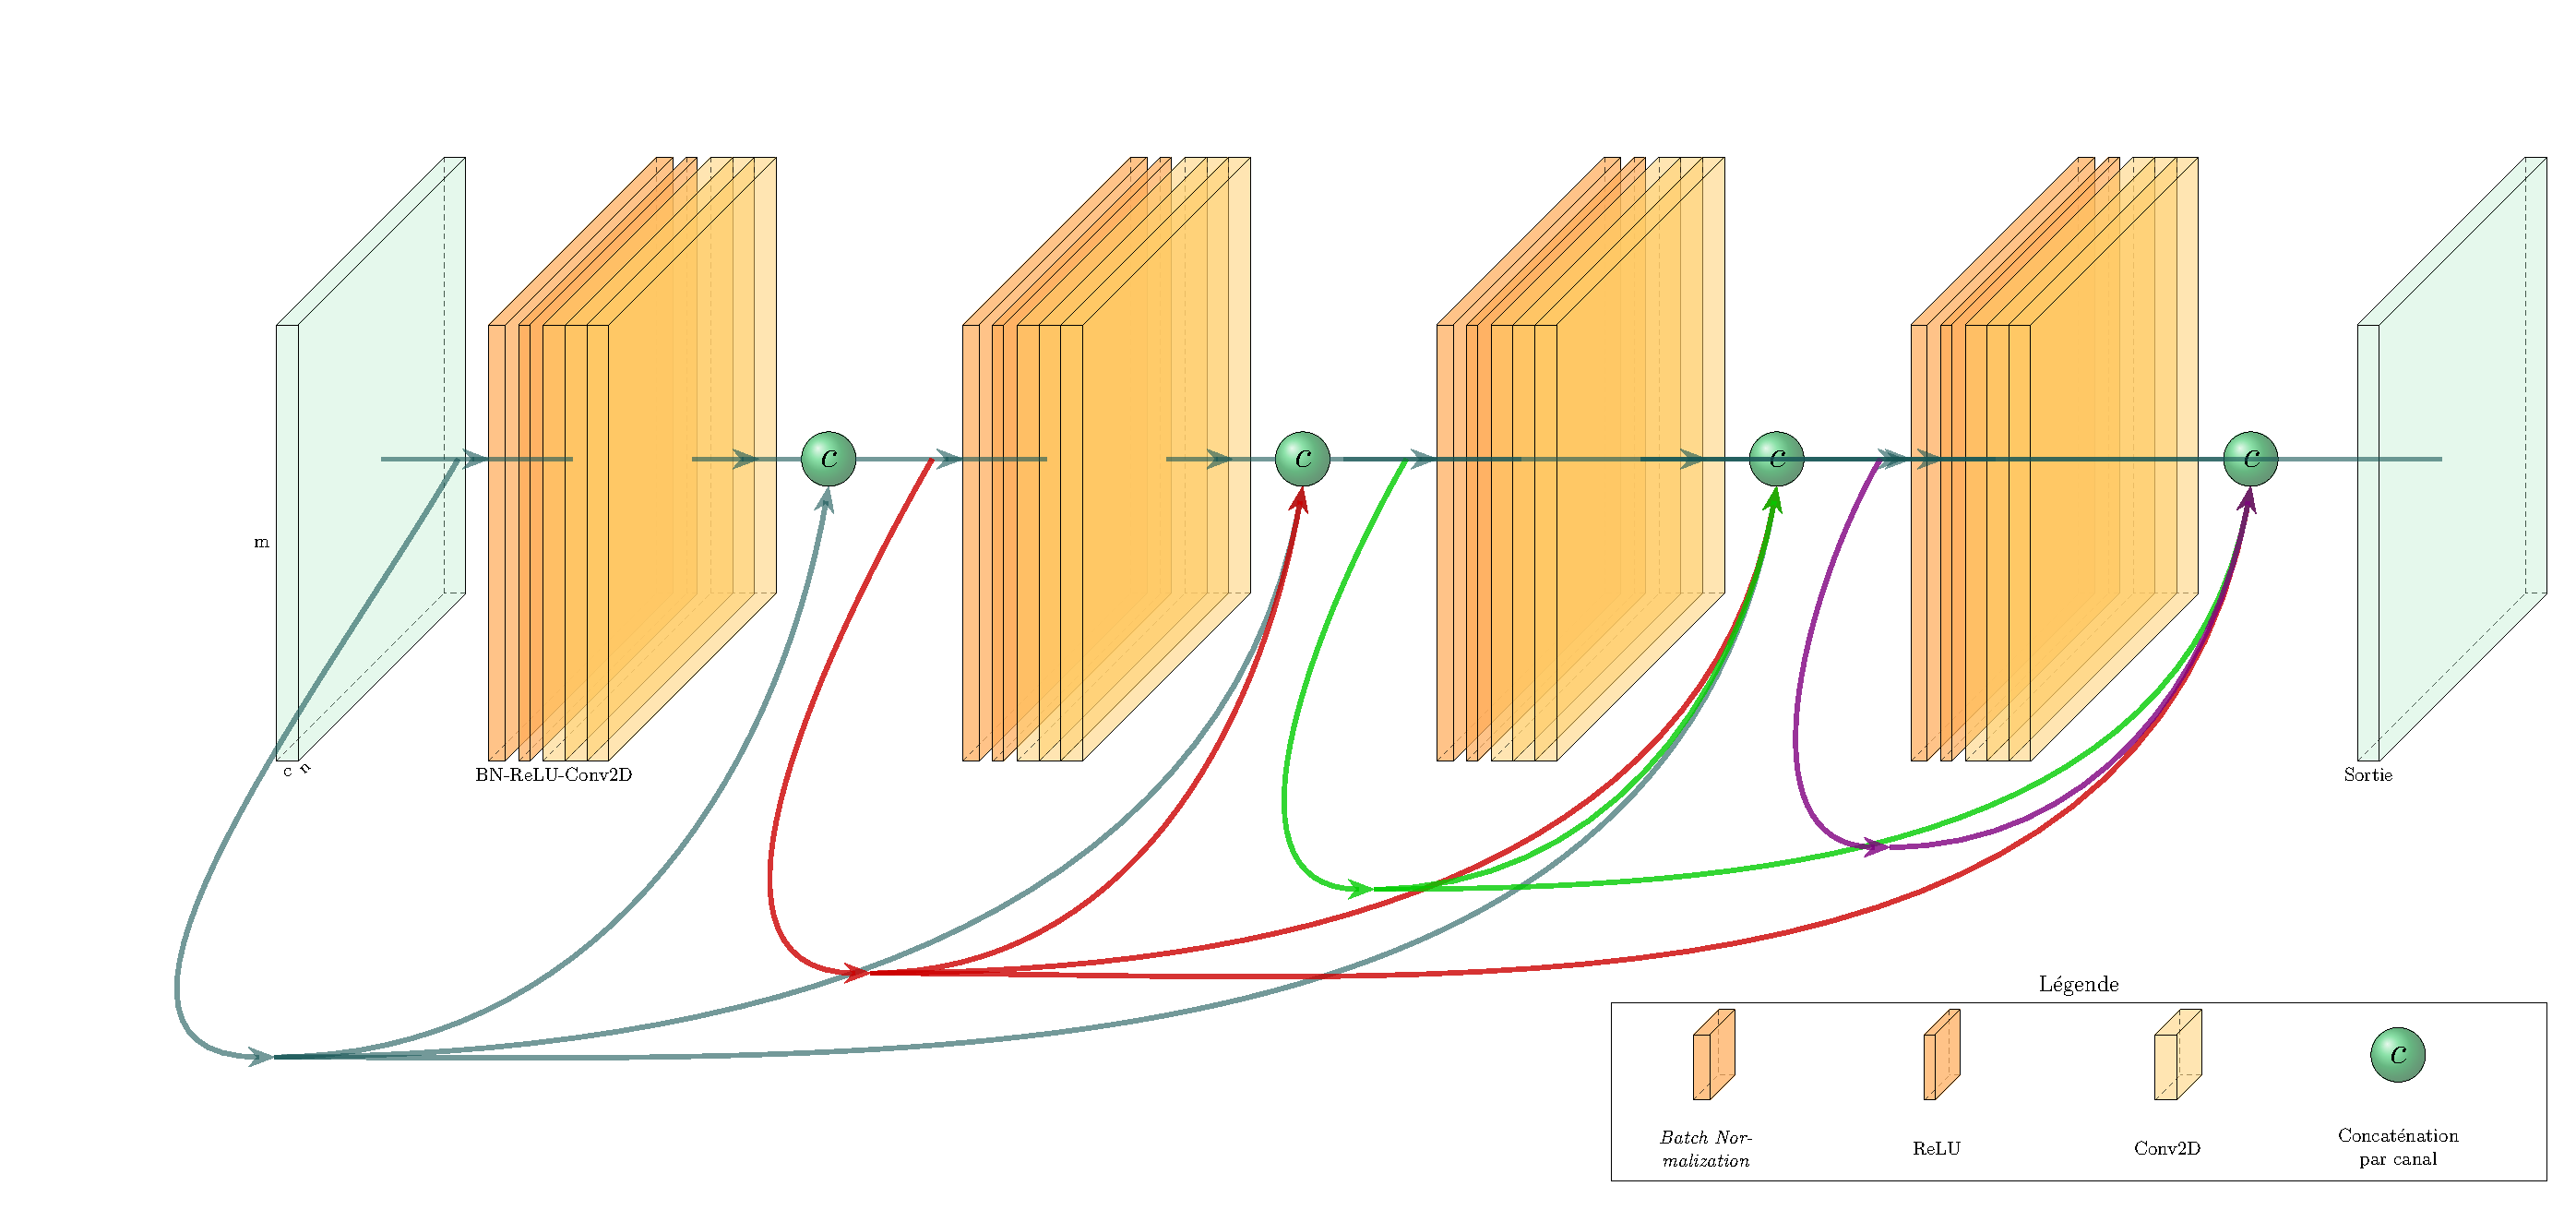
\includegraphics[width=\textwidth,height=\textheight,keepaspectratio]{../Chap4/Figures/densenet.pdf}
	\caption{Architecture d'un bloc DenseNet.}
	\label{fig:densenet}
\end{figure}

La dernière évolution des réseaux résiduels est l'introduction de multiples blocs dans chaque neurones classiques.
C'est l'architecture \textit{ResNext} \cite{xie_aggregated_2016}, une dimension $C$ dite de "cardinalité" qui définit le nombre de bloc présent dans chaque couche. Les auteurs montrent l'intérêt d'une architecture où $c = 32$ : chaque bloc est répété 32 fois par neurones. 

Les performances sont améliorées bien que cela représente une augmentation conséquente des paramètres du réseau.
Dernièrement, \citeauthor{mahajan_exploring_2018} \cite{mahajan_exploring_2018} ont réussi à augmenter les performances sur \textit{ImageNet} en réalisant un pré-apprentissage sur 940 millions d'images issues d'\textit{Instagram}.
La capacité (au sens de la théorie VC \cite{vapnik_principles_1992}) du modèle \textit{ResNext} est bien supérieure à la seule base \textit{ImageNet} et un plus grand nombre de données réelles permet d'augmenter les performances, par la généralisation du problème.

Cependant, l'augmentation du nombre de paramètres des réseaux n'est pas nécessairement significative de meilleures performances.
Dernièrement, le réseau \textit{EfficientNet} dépasse l'état de l'art sur \textit{ImageNet} en diminuant drastiquement le nombre de paramètres ajustables et optimisant sous contrainte l'occupation mémoire et le nombre d'opérations nécessaires.
Précédemment, les réseaux \textit{MobileNetV1} \cite{howard_mobilenets_2017} et \textit{MobileNetV2} \cite{sandler_mobilenetv2_2018} cherchent à obtenir les meilleures performances sur dispositifs embarqués tels que les smartphones.
Il s'agit de limiter le nombre de paramètres et le nombre d'opérations à réaliser (additions et multiplications).
\textit{MobileNetV1} obtient une performance supérieure à \textit{GoogLeNet}, avec trois fois moins d'opérations à réaliser.
Il égale \textit{VGG19} avec trente fois moins d'opérations et dix fois moins d'occupation mémoire.
\textit{MobileNetV1} utilise un bloc de convolution efficient, proposé dans l'architecture \textit{Xception} de \citeauthor{chollet_xception_2016} \cite{chollet_xception_2016} : la convolution est effectuée indépendamment sur chaque canal, avec un poids différent pour chaque canal, puis les résultats sont concaténés.
Pour une convolution traditionnelle de fenêtre $3 \times 3$, la réduction du nombre d'opérations de calcul à effectuer est d'un facteur $9$.
\textit{MobileNetV2} ajoute ensuite l'utilisation de connexions intermédiaires entre chaque couche, à la manière des réseaux résiduels.
Les performances de ces réseaux sont inférieures à l'état de l'art mais ils permettent d'exécuter l'inférence avec des performances satisfaisantes sur des systèmes embarqués.
%TODO: plot deepwise conv
% https://arthurdouillard.com/post/3-small-but-powerful-cnn/
% https://medium.com/@yu4u/why-mobilenet-and-its-variants-e-g-shufflenet-are-fast-1c7048b9618d

\section{Fonctions d'activations} \label{subsubsec:activation}
Pour éviter les deux problèmes de l'explosion ou de l'effondrement de la valeur du gradient pendant l'apprentissage, nous utiliserons dans nos travaux des fonctions d'activation \textit{LeakyReLU}, \textit{PreLU} ou \textit{ELU}, récemment proposées dans la littérature.
La fonction d'activation est une non-linéarité qui suit traditionnellement l'opération de convolutions.
Elle permet de modéliser une réponse à un problème non linéaire.
Les fonctions d'activation historiques sont la tangente hyperbolique et la sigmoïde.
\citeauthor{nair_rectified_2010} \cite{nair_rectified_2010} proposent la fonction \textit{ReLU} (\textit{Rectified Linear Unit}) qui une approximation de la sigmoïde par trois et obtient de meilleures performances, en diminuant le coût du calcul.

\begin{table}[hbtp]
	\centering
	\setlength{\tabcolsep}{2em} % for the horizontal padding
	\renewcommand{\arraystretch}{1.5}% for the vertical padding
	\begin{tabular}{|l|l|l|}
		\hline
		Fonction  & Équation                                                                                                                 & Dérivée                                                                                                            \\ \hline\hline
		Sigmoïde  & $f(x) = \frac{1}{1+e^{-x}}$                                                                                                     & $f(x)(1-f(x))$                                                                                                     \\ \hline
		Tanh      & $tanh(x)  = \frac{2}{1+e^{-2 x}}-1$                                                                                      & $1-f(x)^{2}$                                                                                                       \\ \hline
		ReLU      & $\left\{\begin{aligned} {0} & {\text { si } x<0} \\ {x} & {\text { si } x \geq 0}\end{aligned}\right.$                    & $\left\{\begin{aligned} {0} & {\text { si } x<0} \\ {1} & {\text { si } x \geq 0}\end{aligned}\right.$              \\ \hline
		LeakyReLU & $\left\{\begin{aligned} 0,01 x & \text { si } x<0 \\ x & \text { si } x \geq 0 \end{aligned}\right.$                     & $\left\{\begin{aligned}{0,01} & {\text { si } x<0} \\ {1} & {\text { si } x \geq 0}\end{aligned}\right.$     \\ \hline
		PreLU     & $\left\{\begin{aligned} \alpha x & \text { si } x<0 \\ x & \text { si } x \geq 0 \end{aligned}\right.$                   & $\left\{\begin{aligned}{\alpha} & {\text { si } x<0} \\ {1} & {\text { si } x \geq 0}\end{aligned}\right.$ \\ \hline
		ELU       & $\left\{\begin{aligned} \alpha\left(e^{x}-1\right) & \text { si } x<0 \\ x & \text { si } x \geq 0 \end{aligned}\right.$ & $\left\{\begin{aligned} f(x)+\alpha & \text { si } x<0 \\ 1 & \text { si } x \geq 0 \end{aligned}\right.$          \\ \hline
	\end{tabular}
	\caption{Fonctions d'activation.}
	\label{tab:activations}
\end{table}

Le principal problème est que la fonction \textit{ReLU} vaut zéro pour des valeurs négatives.
C'est pourquoi \citeauthor{maas_rectifier_2013} \cite{maas_rectifier_2013} introduisent le \textit{LeakyReLU} : une succession de deux droites affines, dont la pente de la droite pour les valeurs négatives est non nulle, mais très faible ($0,01 \cdot x$).
Par la suite, \citeauthor{he_delving_2015} \cite{he_delving_2015} introduisent le \textit{PreLU} (\textit{Parametric ReLU}) dont un paramètre $\alpha \geq 0$ définit la pente de la droite pour les valeurs négatives.
$\alpha$ est appris au cours de l'apprentissage tout comme les matrices de poids du réseau.
La valeur de $\alpha$ peut également être indépendante pour chaque canal.
Ces fonctions sont discontinues et ne sont pas dérivables en zéro.
Cela peut entrainer des problèmes de convergence lors de la rétro-propagation du gradient.
C'est pourquoi dernièrement, \citeauthor{clevert_fast_2015} proposent le \textit{ELU} (\textit{Exponential Linear Unit}) qui est dérivable \cite{clevert_fast_2015}.
L'ensemble des graphes de ces fonctions est présenté dans la Figure \ref{fig:activation}, leurs dérivées dans le Tableau \ref{tab:activations}.

\begin{figure}[hbtp]
	\centering
	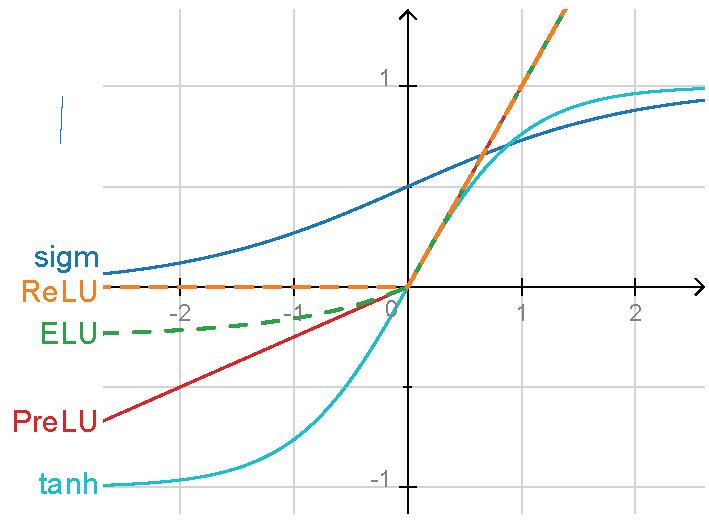
\includegraphics[width=0.7\textwidth,height=0.7\textheight,keepaspectratio]{../Chap4/Figures/activations.pdf}
	\caption{Fonctions d'activation.}
	\label{fig:activation}
\end{figure}
% https://www.mathcha.io/editor
% https://tikzcd.yichuanshen.de/

\section{Méthode de régularisation pour limiter le sur-apprentissage}
Le nombre de degrés de liberté d'un modèle à réseaux de neurones profonds est supérieur à un million.
C'est pourquoi, il est courant que le modèle se spécialise afin d'obtenir un très bon score de justesse sur les échantillons d'apprentissages, mais un mauvais score sur de nouveaux échantillons : c'est le problème du \emph{sur-apprentissage}.
Plusieurs méthodes de régularisation permettent de limiter ce problème et nous détaillerons dans cette section les méthodes que nous utilisons.
\citeauthor{goodfellow_deep_2016} proposent une définition du terme "régularisation", spécifique à l'alchimie du \textit{Deep Learning} \cite{goodfellow_deep_2016} :
\begin{quote}
	« La régularisation est toute modification faite à un algorithme d'apprentissage afin que l'erreur de généralisation soit réduite, mais pas l'erreur d'apprentissage. »
\end{quote}

\subsection{Dropout} \label{parag:dropout}
\citeauthor{srivastava_dropout_2014} \cite{srivastava_dropout_2014} proposent l'utilisation d'une couche dite de \textit{dropout} : la valeur de sortie de cette couche est aléatoirement, selon un pourcentage de chances $\alpha$ choisi, fixée à zéro. Le \textit{dropout} est actuellement la méthode de régularisation la plus performante pour limiter le sur-apprentissage.
Ainsi, l'optimisation est réalisée sur une mauvaise valeur (zéro) de sortie du modèle pour un pourcentage $\alpha$ d'échantillons d'un \textit{mini-batch}.
La valeur de $\alpha$ est souvent fixée entre $[0 ; 0,5]$.
Lors de l'utilisation du modèle pour inférence, la valeur de $\alpha$ est nulle : la couche de \textit{dropout} n'est jamais activée, pour ne pas fausser les prédictions.

\subsection{Normalisation de lots} \label{parag:batchnorm}
La couche de normalisation de lots (\textit{Batch Normalization}) a été proposée par \citeauthor{ioffe_batch_2015} \cite{ioffe_batch_2015}.
Elle nécessite l'emploi de l'entrainement par descente de gradient stochastique qui découpe le jeu de données d'apprentissage en \textit{mini batch} répartis aléatoirement.
On définit les valeurs $x_i$ en entrée de la couche pour un \textit{mini batch} $B \in X$.
On calcule la variance $\sigma_B^2$ de l'entrée et la moyenne $\mu_B$.
La couche \textit{BN} normalise les valeurs des entrées $x_i$ en $\bar{x}_{i}$ par la variance et la moyenne de la distribution du \textit{mini batch}, Équations \ref{eq:batch_norm}.

\begin{equation} \label{eq:batch_norm}
\begin{split}
\mu_{B} \leftarrow \frac{1}{m} \sum_{i=1}^{m} x_{i} , \quad \quad \quad \quad \ \ \ \text{ Moyenne}
\\
\sigma_{B}^{2} \leftarrow \frac{1}{m} \sum_{i=1}^{m}\left(x_{i}-\mu_{B}\right)^{2} , \quad \quad \quad \quad \ \ \ \ \text{  Variance}
\\
\bar{x}_{i} \leftarrow \frac{x_{i}-\mu_{B}}{\sqrt{\sigma_{B}^{2}+\epsilon}} , \text{ Batch normalization} \ 
\end{split}
\end{equation}

La couche \textit{BN} limite les variations importantes de la covariance des entrées. S'il n'y a pas de normalisation, lors de la rétro-propagation, l'ajustement des poids devra être fait pour chaque distribution différente de \textit{mini-batch}.
Avec la normalisation, la sortie aura toujours une distribution normalisée sur zéro et ainsi la valeur des poids à ajuster ne sera pas extrême.
\citeauthor{ioffe_batch_2015} \cite{ioffe_batch_2015} suggère d'utiliser en priorité des couches \textit{BN} plutôt que le \textit{dropout}, car ce dernier fait perdre la totalité de l'information du réseau lorsqu'elle est active, ce qui pénalise fortement la vitesse d'apprentissage.
Les architectures de réseaux profonds antérieures à 2015 (par exemple VGG16) n'utilisent pas de couches \textit{BN}, alors que la majorité des architectures postérieures à 2015 en utilisent.
Lors de l'utilisation du modèle pour inférence, la valeur de $\mu_{B}$ et $\sigma_B^2$ est fixée pour tous les \textit{mini batch} : ce sont leurs moyennes respectives sur tous les \textit{mini batch} de l'entrainement.
% https://arthurdouillard.com/post/normalization/
% How To Be Confident In Your Neural Network Confidence : Temperature Scaling on SoftMax

\subsection{Arrêt prématurée de l'apprentissage} \label{parag:early_stopping}
Cette méthode permet de limiter le sur-apprentissage en stoppant la phase d'apprentissage dès lors qu'il n'y a plus d'amélioration des performances du modèle.
Aussi appelé \textit{early stopping} \cite{yao_early_2007}, il s'agit de trouver le nombre optimal d'itérations successives pour ne pas sur-apprendre le jeu de données d'apprentissage.
Pour cela, le jeu de données initial est séparé en une partition d'apprentissage et une partition de validation.
L'apprentissage du modèle est effectué en utilisant la partition d'apprentissage.
À chaque itération, la performance du modèle est évaluée sur la partition de validation, inconnue du modèle.
Si la performance de validation a été améliorée, alors l'itération d'apprentissage a amélioré le modèle.
En revanche, si la performance de validation est moins bonne qu'à l'itération précédente, le modèle a été dégradé pour la partition de validation.
C'est pourquoi, il aurait été judicieux de ne pas effectuer cette itération qui a dégradé le modèle, et de conserver le modèle tel que précédemment : c'est ce que réalise le \textit{early stopping}.
L'algorithme de descente de gradient peut souvent produire une mauvaise performance pendant quelques itérations avant d'améliorer le modèle, c'est pourquoi on introduit le terme de patience $p$ : le nombre d'itérations qui n'améliore pas le modèle, avant de terminer l'apprentissage.
La performance de cette méthode dépendra du choix judicieux de l'hyper-paramètre $p$, c'est pourquoi il est obligatoire de trouver la valeur de $p$ optimale pour le problème à résoudre, §\ref{sec:auto_ml}.

\subsection{Réduction de dimensions par interpolation} \label{parag:pooling}
L'idée principale de l'architecture des réseaux de neurones profonds (avant la proposition des réseaux résiduels) est de réduire successivement, à chaque couche, la dimension des vecteurs, afin de réduire le nombre de paramètres des couches. Cela réduit les coûts des calculs et le risque de sur-apprentissage.
Les couches de convolutions appliquent un filtre mais ne réduisent pas la dimension.
C'est pourquoi elles sont suivies de couches dites de \textit{pooling}. Parmi les nombreuses fonctions de \textit{pooling} proposées, on distingue les deux principales : le sous-échantillonnage par moyenne, et la seule conservation de la valeur maximale, le \textit{max pooling}, Tableau \ref{tab:maxpooling}.
Cette couche est appliquée sur un certain nombre de valeurs adjacentes.
Des dimensions courantes sont de $2 \times 2$ à $4 \times 4$, en fonction de la dimension des caractéristiques des échantillons que l'on cherche à mettre en valeur.
Une fenêtre de $2 \times 2$ réduit la dimension d'un facteur 4.

\begin{table}[hbtp]
	\centering
	\begin{tabular}{|c|c||c|c|}
		\hline
		0 & \textbf{255} &          10 &            0 \\ \hline
		10 &           20 &           0 & \textbf{200} \\ \hline \hline
		\textbf{50} &            0 &           0 &            0 \\ \hline
		10 &            0 & \textbf{20} &           10 \\ \hline
	\end{tabular}
	\quad
	$\rightarrow$
	\quad
	\begin{tabular}{|c||c|}
		\hline
		\textbf{255} & \textbf{200} \\ \hline \hline
		\textbf{50}  & \textbf{20}  \\ \hline
	\end{tabular}
	\caption{Illustration d'une couche de \emph{max pooling}.}
	\label{tab:maxpooling}
\end{table}

\citeauthor{boureau_theoretical_2010} \cite{boureau_theoretical_2010} analysent l'influence du choix de la fonction et montre la supériorité du \textit{max pooling} lorsque les valeurs à détecter sont peu fréquentes.
\citeauthor{scherer_evaluation_2010} \cite{scherer_evaluation_2010} obtient également des performances supérieures avec le \textit{max pooling} qui permet d'extraire les caractéristiques de petites dimensions spatiales.
Une particularité du \textit{max pooling} est d'être très simple à calculer lors de la rétro-propagation : seul le poids associé à la valeur maximale est ajusté.
La Figure \ref{fig:pooling} illustre l'effet du \textit{max pooling} et de l'\textit{average pooling} pour quatre filtres de convolutions différents.

\begin{figure}[hbtp]%[!h]
	\centering
	\begin{subfigure}[c]{0.2\textwidth}\label{fig:imgA_gray}
		\centering
		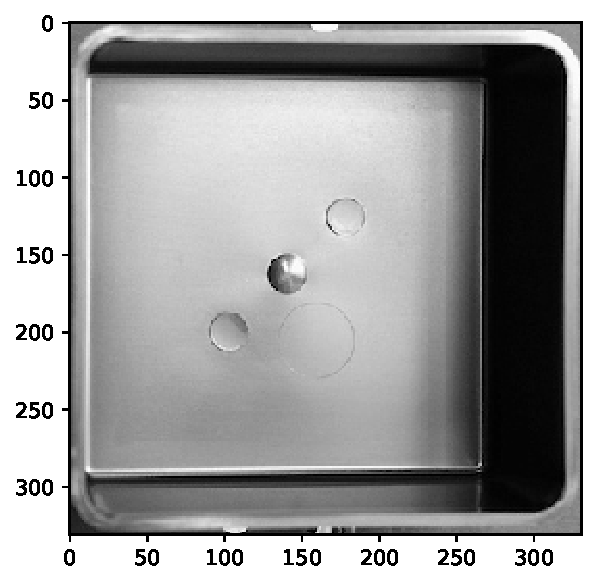
\includegraphics[width=\textwidth]{../Chap4/Figures/imgA_gray.pdf}
		\caption{Image originale.}
	\end{subfigure}
	$\otimes$  % $\Huge \otimes$
	\begin{subfigure}[c]{0.76\textwidth}
		\centering
		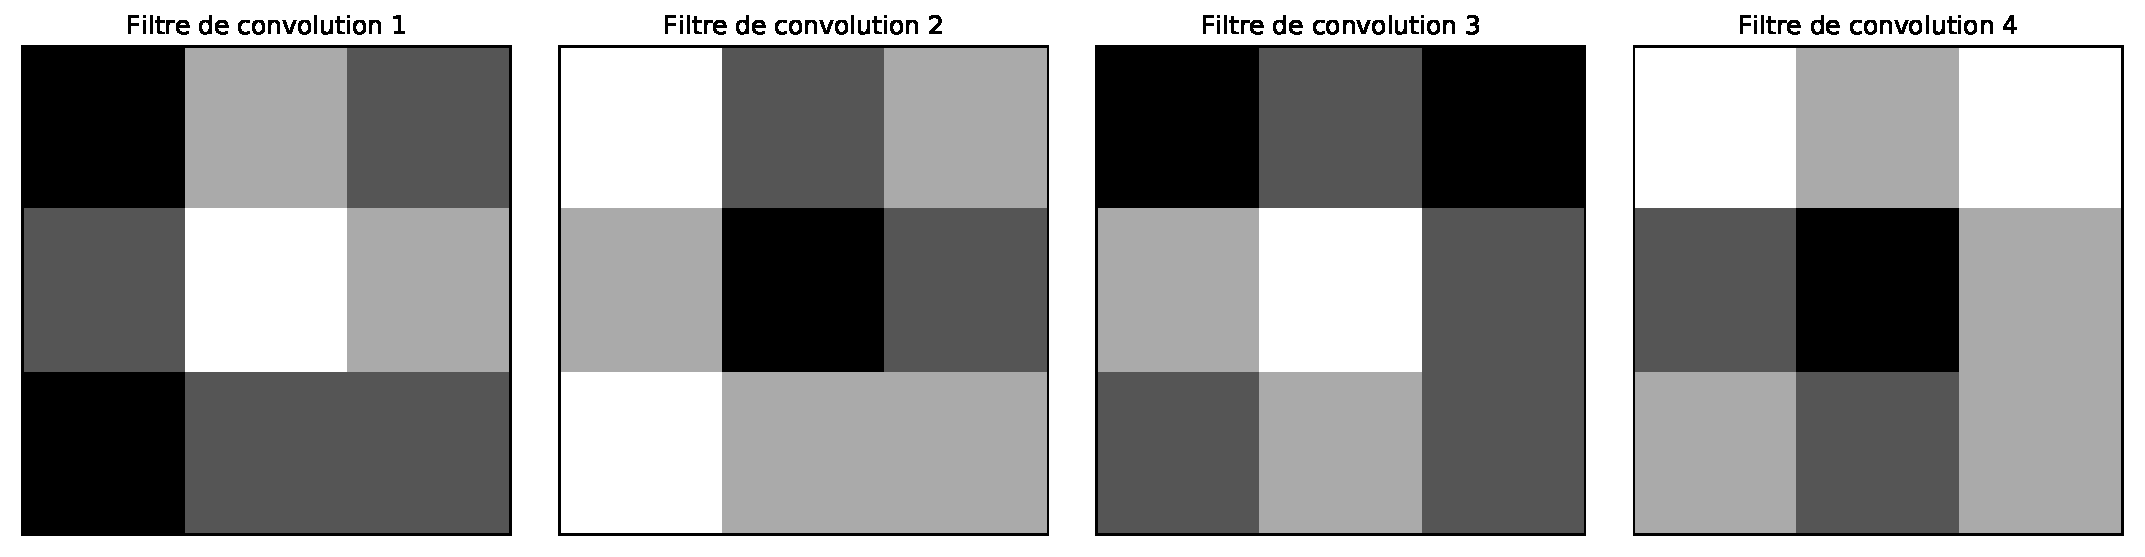
\includegraphics[width=\textwidth]{../Chap4/Figures/imgA_filters.pdf}
		\caption{Filtres de convolutions appliqués.}
		\label{fig:conv_filters}
	\end{subfigure}%  \hspace{20mm}%
	%\hspace{1em}% Space between image A and B
	\vspace{1.2\baselineskip}
	\begin{subfigure}[c]{1\textwidth}
		\centering
		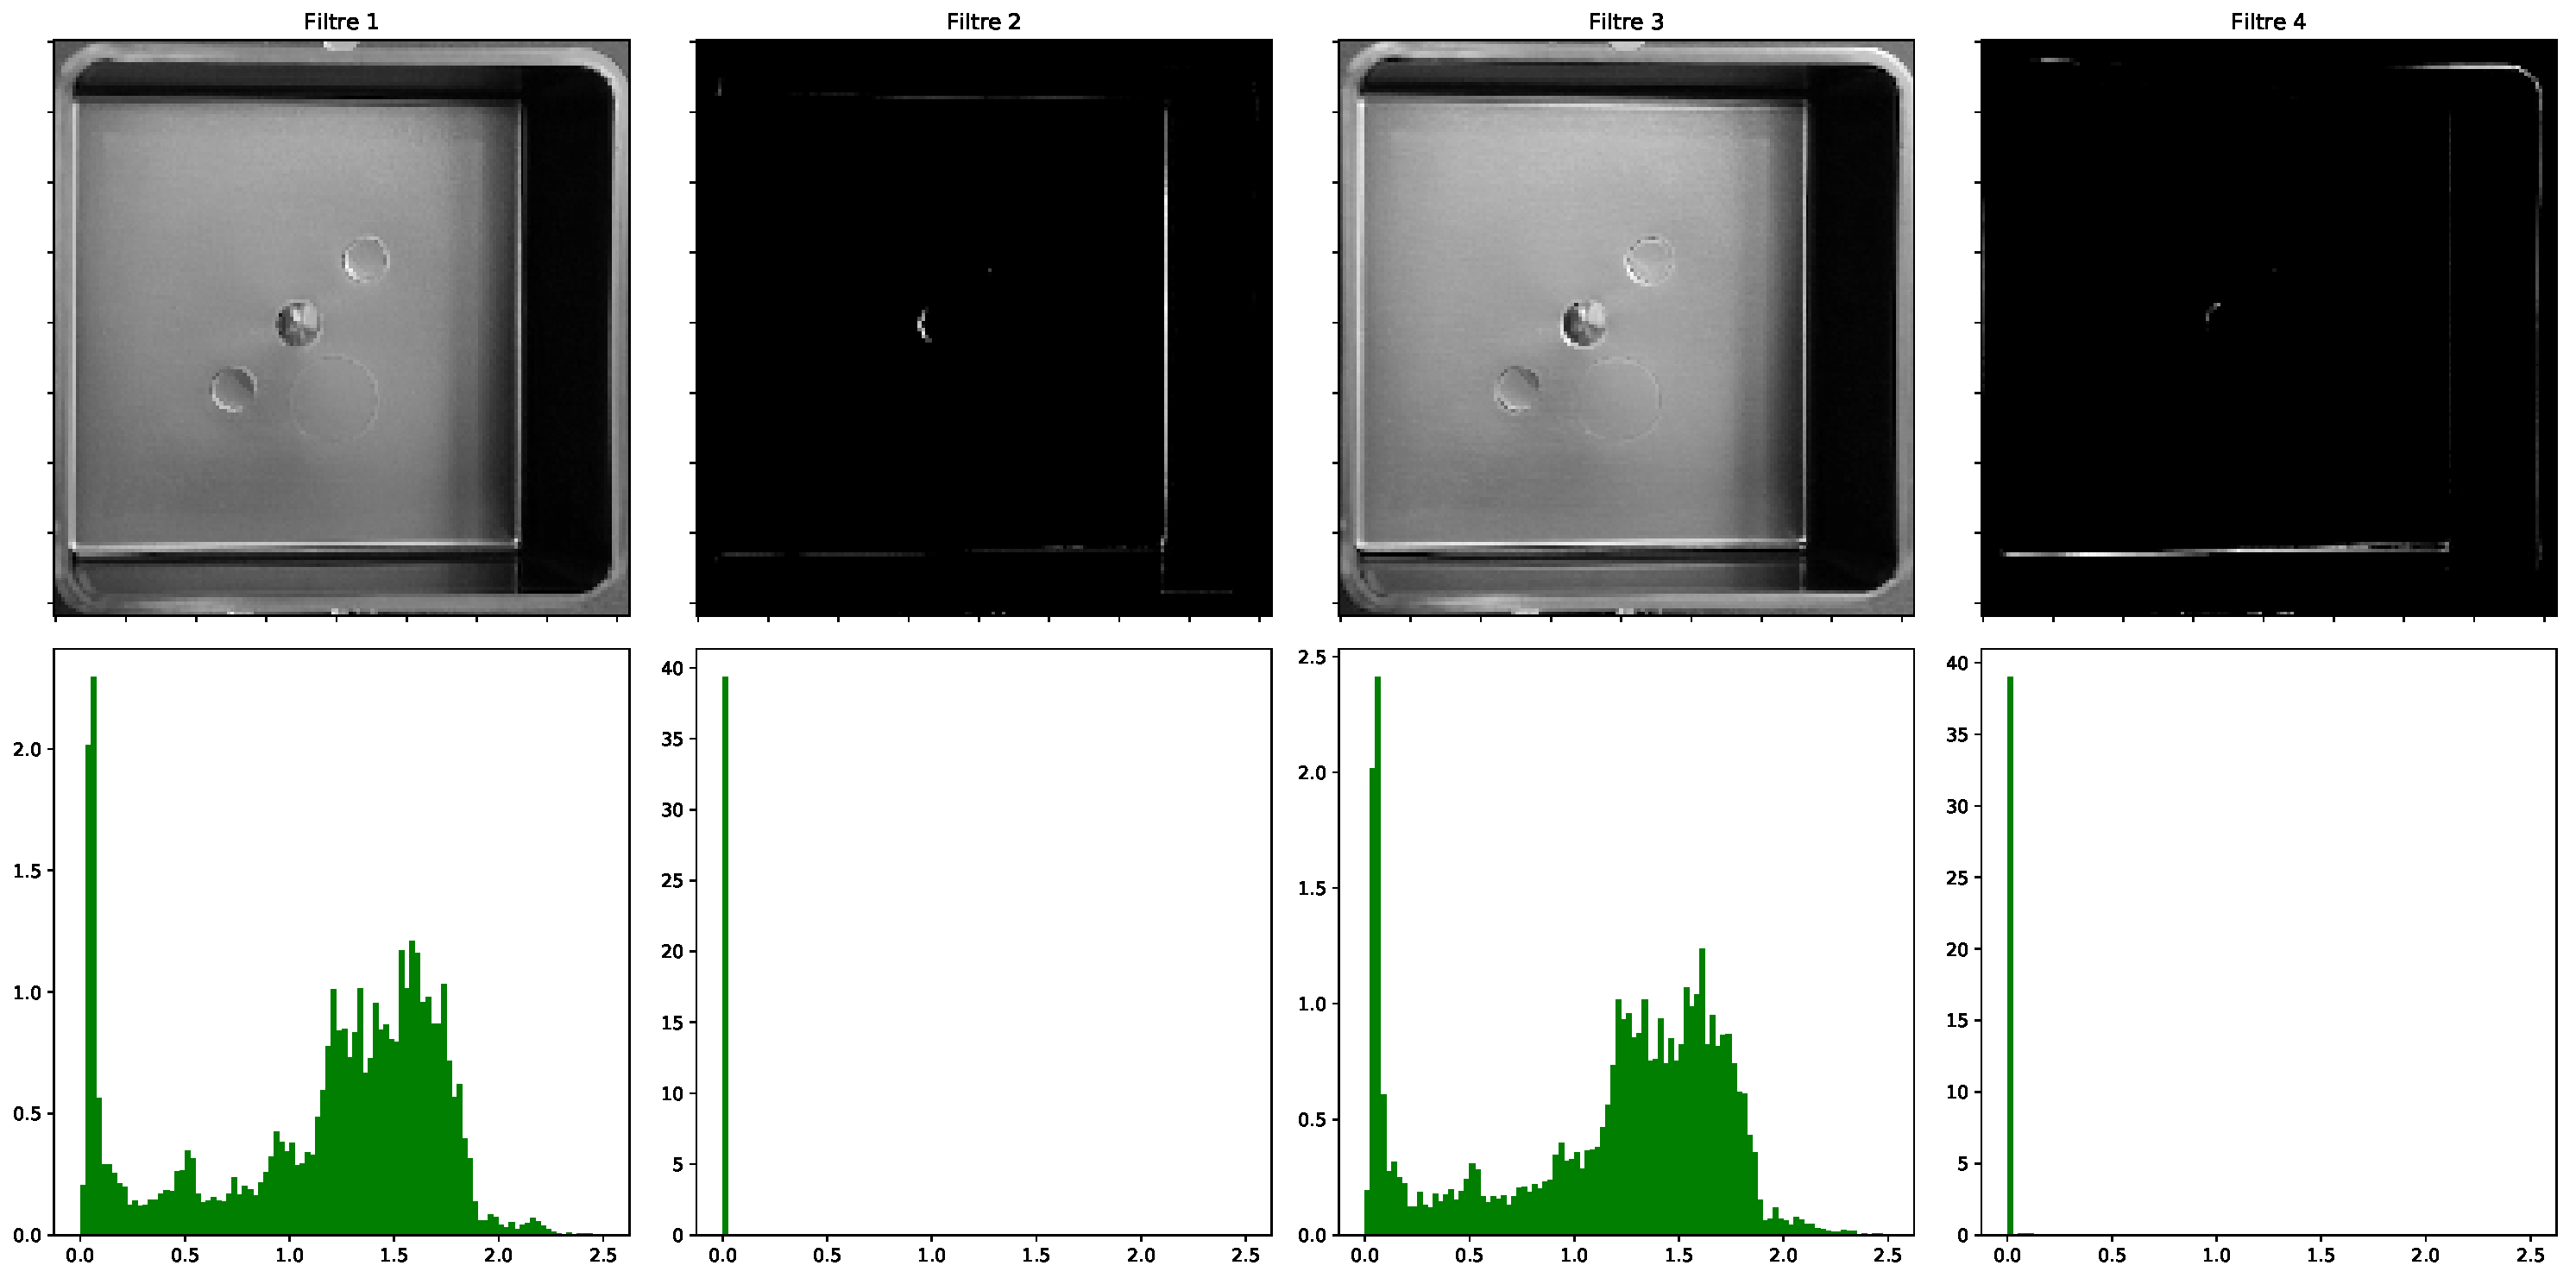
\includegraphics[width=\textwidth]{../Chap4/Figures/imgA_maxpool.pdf}
		\vspace{-0.9\baselineskip}
		\caption{Sorties avec \emph{max pooling}.}
		\label{fig:max_pool}
	\end{subfigure}%
	\vspace{1.2\baselineskip}
	\begin{subfigure}[c]{1\textwidth}
		\centering
		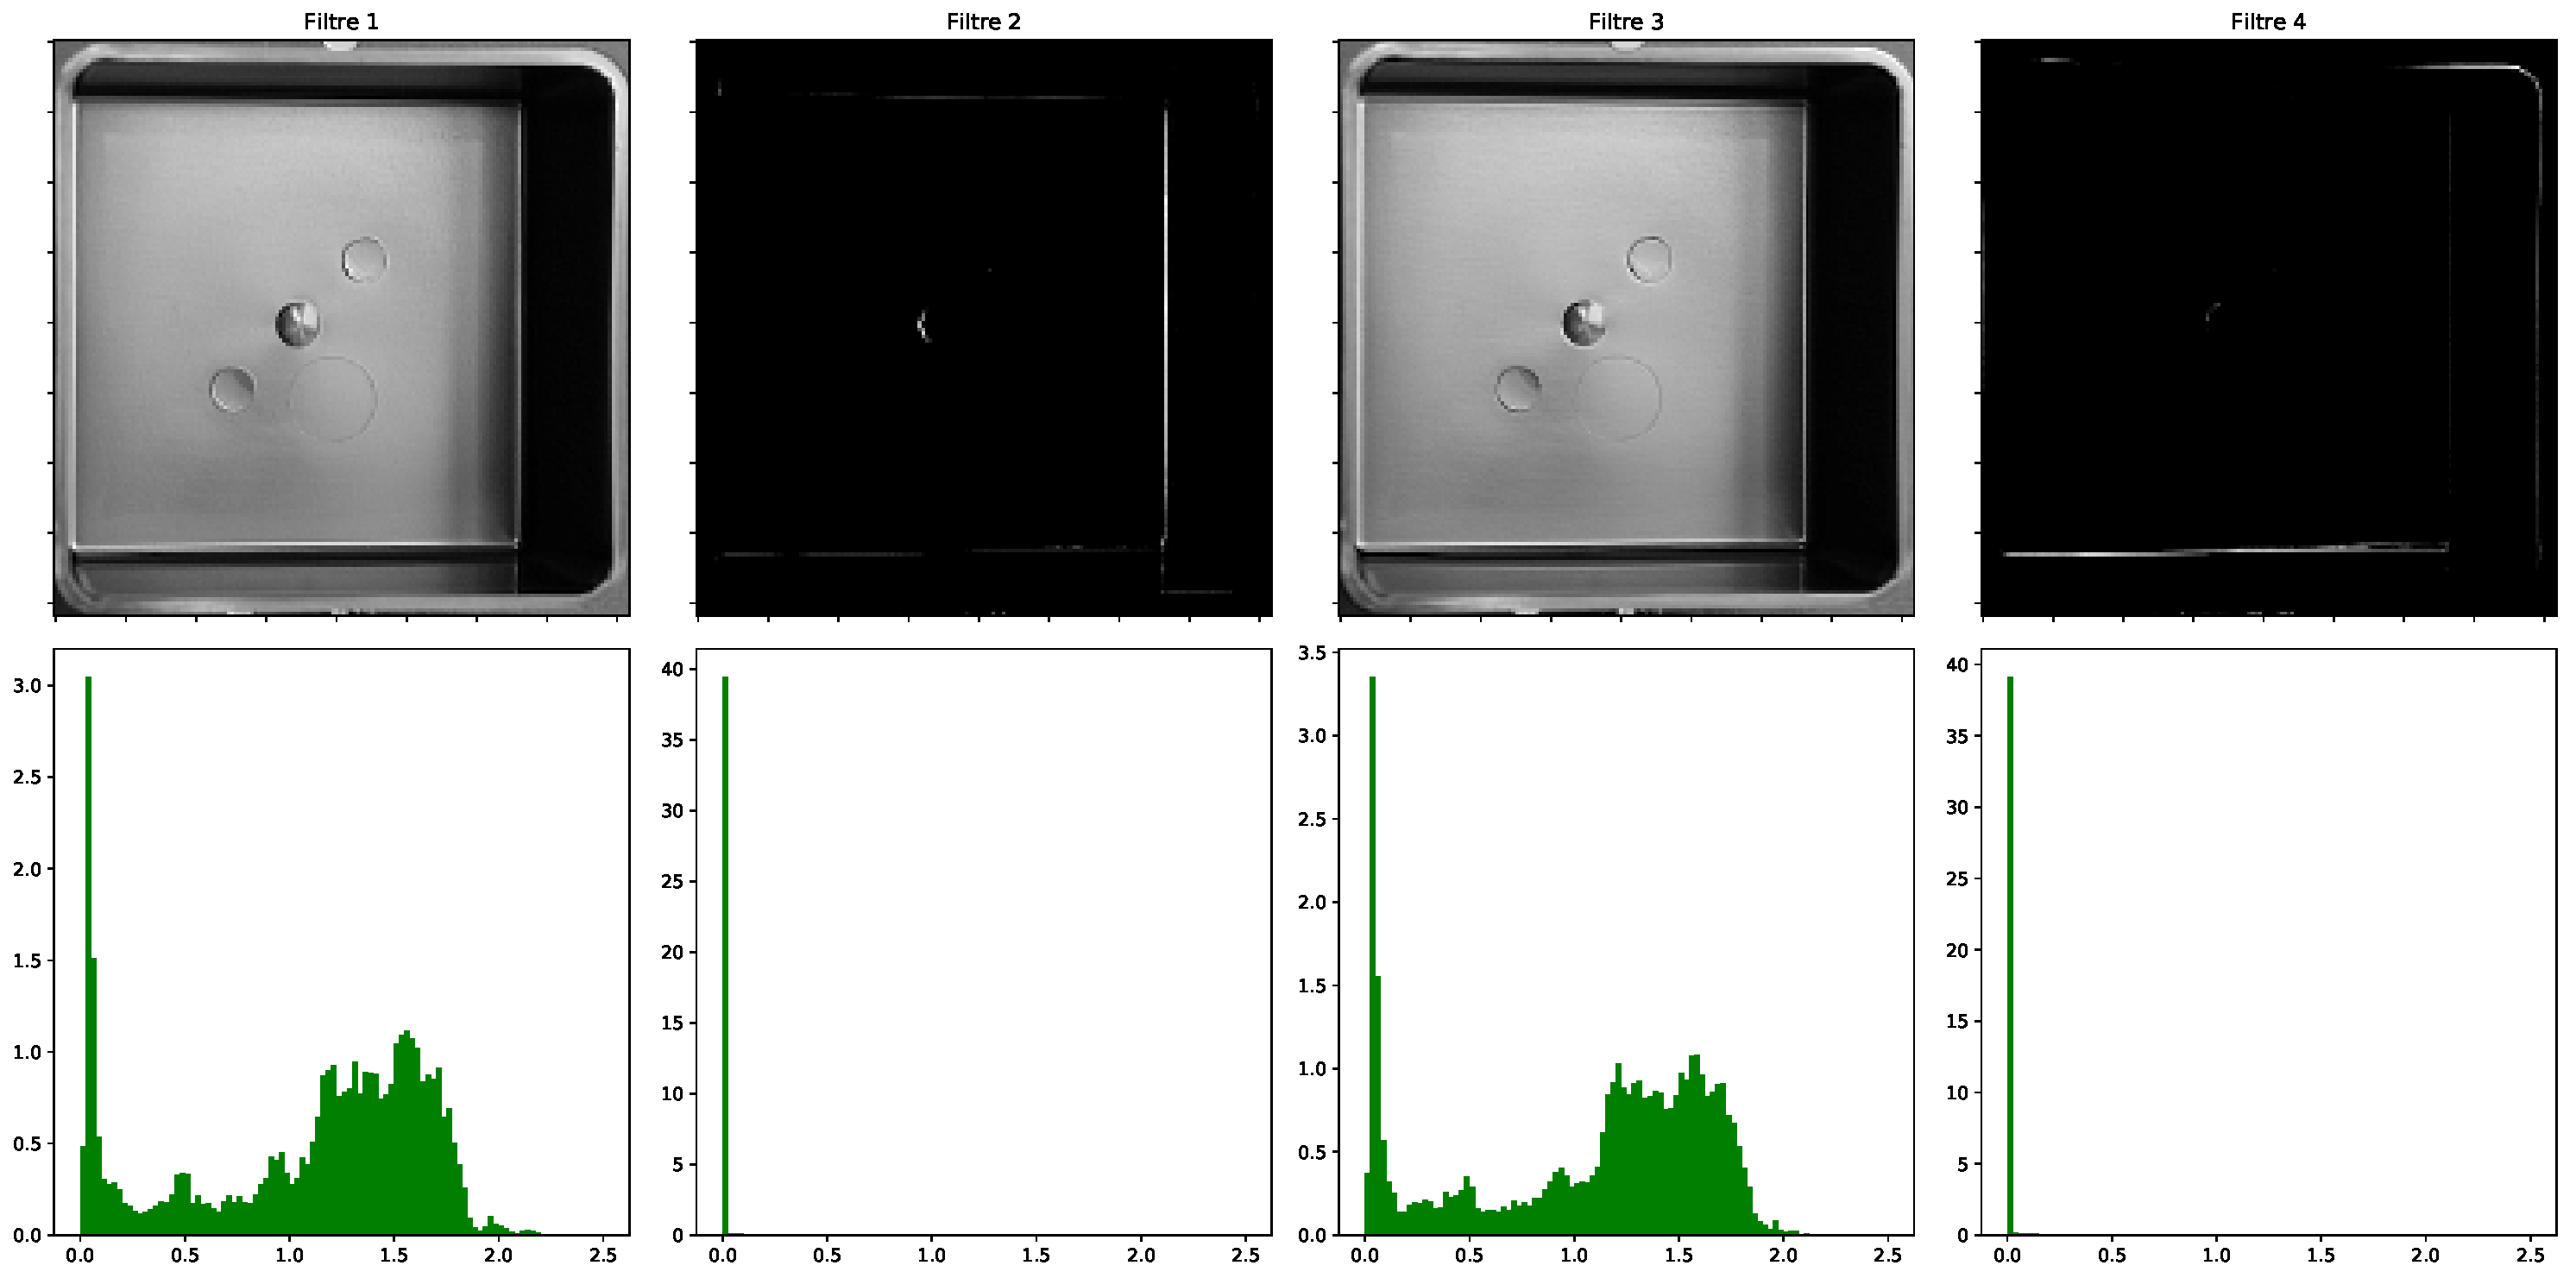
\includegraphics[width=\textwidth]{../Chap4/Figures/imgA_avgpool.pdf}
		\vspace{-0.9\baselineskip}
		\caption{Sorties avec \emph{average pooling}.}
		\label{fig:avg_pool}
	\end{subfigure}%
	\caption{Comparaison \emph{max pooling} \protect\subref{fig:max_pool} et \emph{average pooling} \protect\subref{fig:avg_pool} pour 4 filtres de convolutions \protect\subref{fig:conv_filters}.}
	\label{fig:pooling}
\end{figure}

\citeauthor{oquab_object_2015} \cite{oquab_object_2015} étudie l'utilisation du \textit{global max pooling} : seule une unique valeur maximale de la couche présente $z$ est conservée, Équation \ref{eq:GMP}.
Cela fait émerger une propriété intéressante : la possibilité d'utiliser la valeur de la couche précédente $z$ comme une carte de saillance de la localisation des différentes classes.
Cette carte est générée à partir d'un jeu de données sans information sur la localisation des objets, de manière semi-supervisée.
La couche de \textit{global max pooling} force le réseau à détecter la position de la meilleure classe dans l'image.

\begin{equation} \label{eq:GMP}
y_{i+1}=\max _{j, k} z_{j, k}(y_i)
\end{equation}

De récentes analyses montrent que le \textit{max pooling} est une source majeure de perte d'information, ce qui peut limiter les performances, particulièrement pour les réseaux génératifs.
C'est pourquoi les architectures récentes cherchent à le remplacer par des couches de sous-échantillonnage par moyenne (\textit{average pooling}).
Dans son réseau composé de sous blocs denses, \cite{lin_network_2013} introduit le \textit{Global Average Pooling}, Équation \ref{eq:GAP}.
\cite{zhou_learning_2015} montre l'intérêt du \textit{Global Average Pooling} lors de l'apprentissage, ce qui permet d'obtenir des cartes de saillance de la localisation des objets dans l'image.
Cette démarche est similaire aux travaux de \citeauthor{oquab_object_2015} \cite{oquab_object_2015} avec le \textit{global max pooling}, mais l'utilisation de la moyenne force le réseau à détecter l'ensemble des régions où la classe est présente.
Cette carte de saillance par classes $z$ est nommée \textit{Class Activation Map}.

\begin{equation} \label{eq:GAP}
y_{i+1} = \frac{1}{N} \sum_{j, k} z_{j, k}(y_i)
\end{equation}

% Les développements des cartes de saillance relèvent de l'apprentissage faiblement supervisé que nous développons dans la partie 
% http://webia.lip6.fr/~cord/pdfs/news/2017CordPoolingDeepNets.pdf

\subsection{Pénalisation sur les poids} \label{parag:weights_decay}
Proposé par \citeauthor{krogh_simple_1991} \cite{krogh_simple_1991}, il s'agit d'ajouter un terme de pénalisation $E$ de la valeur des poids à la fonction de coût $\mathcal{L}$ que l'on cherche à optimiser.
Un facteur $\lambda$ pondère la valeur des poids $\mathbf{W}$ du réseau.
Cette méthode permet de rendre le réseau robuste aux perturbations ce qui améliore les performances.
C'est une méthode simple et efficace, dont l'utilisation est indispensable pour atteindre les performances de l'état de l'art de la littérature.
La pondération peut être effectuée sur la norme $\ell_{1}$, ce qui pénalisera tous les poids différents de zéro.
Mais la pondération est généralement réalisée sur la norme $\ell_{2}$, ce qui pénalisera les grandes valeurs des poids.
Dans ce cas, cette démarche est équivalente à la régularisation de \citeauthor{tikhonov_stability_1943} \cite{tikhonov_stability_1943, tikhonov_solutions_1977} par une matrice $\Gamma$, avec $\Gamma=\lambda I$.
On cherche à amener un maximum de poids du réseau à zéro.
La méthode est d'autant plus critique que les erreurs d'arrondis, inhérentes à la représentation des nombres informatiques, doivent être évitées lors de l'optimisation par descente du gradient.

\begin{equation}
E(\mathbf{W})=E_{0}(\mathbf{W}) + \frac{1}{2} \lambda \sqrt{\sum_{i} \mathbf{w}_{i}^{2}}
\end{equation}

\subsection{Augmentation artificielle du jeu de données} \label{parag:data_augmentation}
La plus simple des méthodes existantes pour limiter le sur-apprentissage est de disposer d'un jeu de données comportant une grande variété d'échantillons par classe. \textit{ImageNet} propose 2000 échantillons par classe.
Récemment, \textit{ResNext\_wsl} \cite{mahajan_exploring_2018} est entrainé sur plusieurs millions d'images par classe.
Lorsque que l'on ne dispose pas de suffisamment de données, il est possible d'augmenter les données existantes.
Il s'agit d'effectuer des transformations affines ou non linéaires, rotations, cadrages ou d'ajouter du bruit dans les images.
L'objectif est d'augmenter la variance du jeu de données initial.
Les taux de modifications optimaux doivent être choisis par validation croisée pour obtenir les meilleures performances possibles sur le problème spécifique.
Nous observons de bonnes performances avec des rotations jusqu'à cinq degrés et des cadrages qui varient de dix pour-cent des dimensions originales, illustrés dans la Figure \ref{fig:augmentor}.

\begin{figure}[htbp]
	\centering
	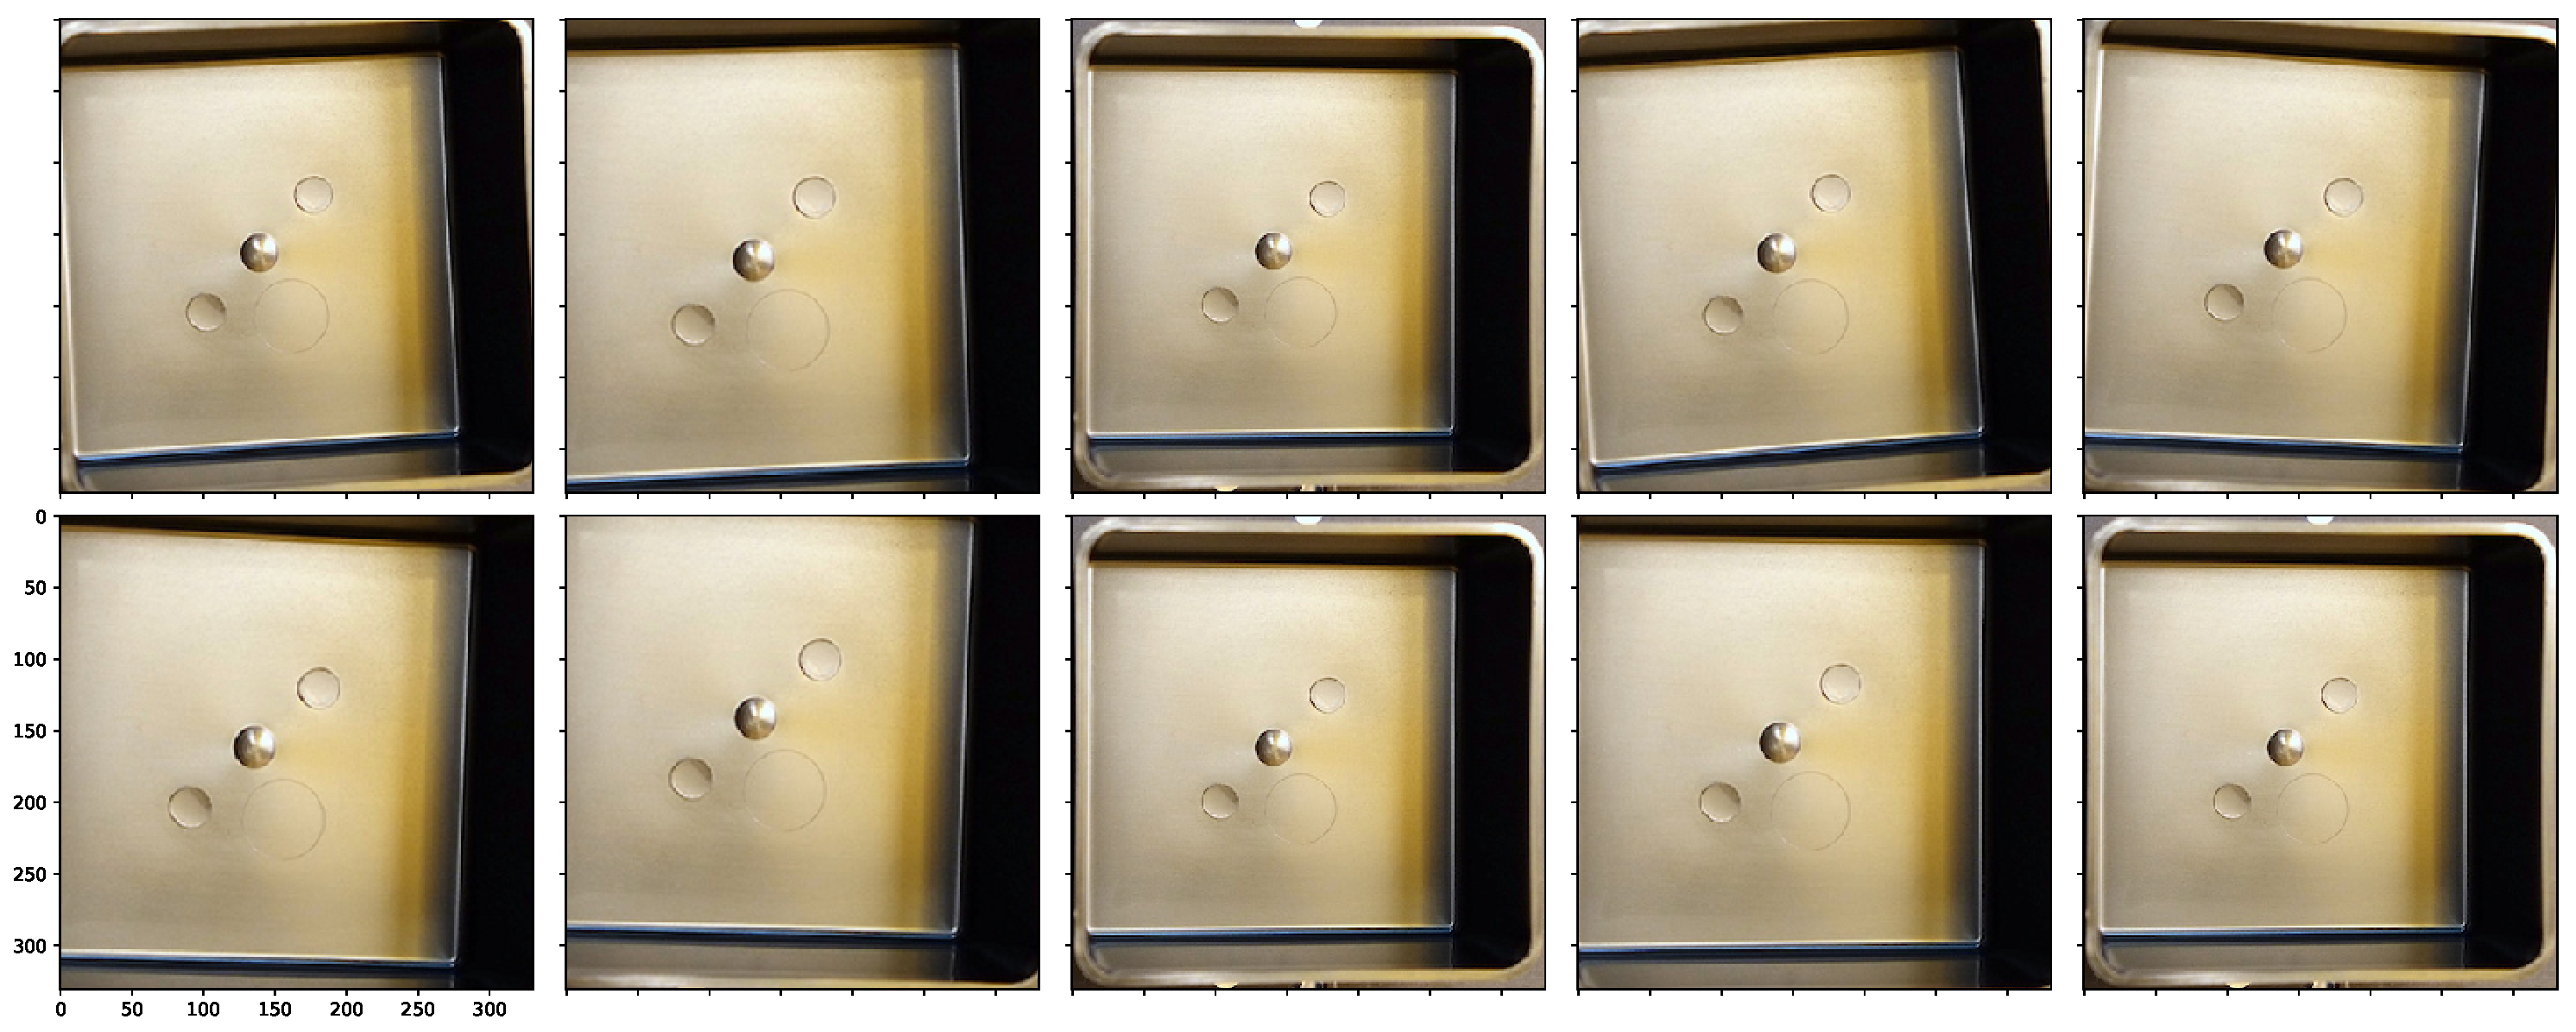
\includegraphics[width=\textwidth,height=\textheight,keepaspectratio]{../Chap4/Figures/imgA_augmentor.pdf}
	\caption{Augmentation d'une image par translations et rotations.}
	\label{fig:augmentor}
\end{figure}

Le choix des paramètres d'augmentation peut être effectué par validation croisée afin d'optimiser les performances.
On préférera se rapprocher des situations réelles de production des données.
Dans notre cas d'application industrielle du contrôle qualité, de légères variations de cadrage, rotation ou de perspectives peuvent exister.
En revanche, nous travaillons avec un éclairage contrôlé, donc les perturbations d'éclairage ou de colorimétrie sont peu probables.
Les paramètres de l'augmentation du jeu de données dépendent de la connaissance du métier.
Si la connaissance du métier n'est pas certaine, il est préférable d'acquérir un plus grand nombre d'images réelles, plutôt que de générer des données artificielles avec de mauvais a priori.

\section{Apprentissage par transfert de domaine} \label{subsec:transfer_learning}
% https://ireneli.eu/2018/08/09/transfer-learning-materials/

Le faible nombre d'échantillons disponibles (inférieur à mille pièces) nous a conduit à utiliser des réseaux de neurones profonds préalablement entrainés sur des très grands jeux de données.
Le jeu de données \textit{ImageNet} \cite{deng_imagenet_2009} est composé de 2 millions d'images réparties en 1000 catégories différentes.
L'apprentissage par transfert de domaine, aussi résumé "apprentissage par transfert", cherche à réutiliser un modèle spécialisé sur un certain problème, pour résoudre un autre problème.
En pratique, les meilleures approches proposées dans la littérature nécessitent de conserver des caractéristiques fortes entre les deux domaines.
% Nous recommandons l'utilisation du même format de données initiales.
Nous nous contenterons ici d'utiliser des modèles spécialisés sur l'analyse d'images à trois canaux de couleurs, et de les spécialiser sur notre propre problématique.

Dans ce cadre d'apprentissage par transfert de domaine, nous n'avons pas la liberté de modifier l'architecture du réseau pré-appris, car il faudrait alors réapprendre les poids des neurones du réseau.
La technique répandue est alors de supprimer la ou les dernières couches du réseau pré-appris et d'ajouter de nouvelles couches spécifiques à notre problème.
Les dernières couches du réseaux sont considérées comme étant le véritable classifieur.
Les couches précédentes se contentent de compresser l'information en une représentation dans un espace de dimensions réduites.
Nous travaillons uniquement sur l'architecture du classifieur, c'est à dire de la fin du réseau.
Le choix de l'architecture et de la typologie des couches influence fortement la performance du classifieur, c'est pourquoi des méthodes de sélections automatiques de ces paramètres doivent être employées.
Elles sont discutées dans la Section \ref{sec:auto_ml}.

On distingue deux étapes successives à l'entrainement d'un réseau de neurones par transfert : l'entraînement des nouvelles dernières couches, puis la spécialisation de l'ensemble du réseau.
Il s'agit dans un premier temps de garantir la convergence du classifieur sur notre problème.
On cherche à obtenir un score de classification satisfaisant.
C'est pourquoi dans un premier, seuls les poids des neurones des nouvelles dernières couches sont ajustés par rétro-propagation du gradient de l'erreur.
Une fois que la convergence des dernières couches a été obtenue, il est possible de spécialiser finement l'ensemble du réseau en réalisant un ajustement de l'ensemble des poids des couches afin d'améliorer le score de classification.
Nos travaux ont montré que cette étape de spécialisation n'est pas nécessaire lorsque le jeu de données d'apprentissage est petit (inférieur à mille échantillons).
En effet, nous n'observons pas d'augmentation du score de classification après la phase de spécialisation.
De plus, la durée de l'apprentissage de spécialisation est deux ordres de grandeur plus longue que la durée de l'apprentissage des dernières couches du réseau, car le nombre de variables à ajuster sur l'ensemble du réseau est bien plus grande.
La durée de l'apprentissage des dernières couches du réseau est de dix secondes sur un processeur graphique récent et puissant (\textit{NVIDIA GTX1080Ti}, 2017).
La durée de l'apprentissage de spécialisation est de dix minutes.
Cette durée rend l'apprentissage de spécialisation compatible avec une mise à jour horaire du classifieur, sous réserve de disposer d'un processeur graphique adapté. L'apprentissage des dernières couches peut en revanche être réalisé en cycle de production, pièce après pièce.
Un classifieur de la conformité qui utilise l'apprentissage par transfert sera adapté aux productions dans lesquels les changements de séries ou bien la dérive du procédé est supérieure à l'heure. Ce qui est compatible avec une mise à jour régulière du modèle de la conformité.